%%%%%%%%%%%%%%%%%%%%%%%%%%%%%%%%%%%%%%%%%%%%%%%%%%%%%%%%%%%%%%%%%
% Contents: Main Input File of the LaTeX2e Introduction
% $Id$
%%%%%%%%%%%%%%%%%%%%%%%%%%%%%%%%%%%%%%%%%%%%%%%%%%%%%%%%%%%%%%%%%
% lshort.tex - Une courte (?) introduction a LaTeX2e
%                                                      by Tobias Oetiker
%                                                     oetiker@ee.ethz.ch
%
%                           based on LKURTZ.TEX Uni Graz & TU Wien, 1987
%                           traduit en français par Matthieu Herrb,1996
%                           puis par Samuel Colin, 2009
%-----------------------------------------------------------------------
%
% To compile lshort, you need TeX 3.x, LaTeX and makeindex
%
% The sources files of the Intro are:
%      lshort.tex, lshort-a5.tex,
%      lshort-base.tex (this file),
%      title.tex, contrib.tex, biblio.tex, graphic.tex
%      things.tex, typeset.tex, math.tex, lssym.tex, spec.tex,
%      lshort.sty, fancyheadings.sty, mylayout.sty
%
% Further the  verbatim.sty and the layout.sty 
% from the LaTeX Tools distribution is
% required.
%
%
% To print the AMS symbols you need the AMS fonts and the packages
% amsfonts, eufrak and eucal from (AMS LaTeX 1.2)
%
% ---------------------------------------------------------------------

% Pour les informations de licence, voir contrib.tex.
% See contrib.tex for license information.

%%%%%%%%%%%%%%%%%%%%%%%%%%%%%%%%%%%%%%%%%%%%%%%%%%%%%%%%%%%%%%%%%
% Contents: Who contributed to this Document
% $Id: contrib.tex 533 2015-04-09 13:00:40Z oetiker $
%%%%%%%%%%%%%%%%%%%%%%%%%%%%%%%%%%%%%%%%%%%%%%%%%%%%%%%%%%%%%%%%%
\begin{small} 
  \noindent Copyright \copyright 1995-2011 Tobias Oetiker and Contributors.  All rights reserved.
 
  This document is free; you can redistribute it and/or modify it
  under the terms of the GNU General Public License as published by
  the Free Software Foundation; either version 2 of the License, or
  (at your option) any later version.
  
  This document is distributed in the hope that it will be useful, but
  \emph{without any warranty}; without even the implied warranty of
  \emph{merchantability} or \emph{fitness for a particular purpose}\@.  See the GNU
  General Public License for more details.
  
  You should have received a copy of the GNU General Public License
  along with this document; if not, write to the Free Software
  Foundation, Inc., 675 Mass Ave, Cambridge, MA 02139, USA.

\vspace{4ex}

  Copyright \copyright{} 1995-2011 Tobias Oetiker et les contributeurs.

  Copyright \copyright{} 1998-2001 LAAS/CNRS pour la traduction
  jusqu'� la version 3.20 incluse.

  Copyright \copyright{} 2009-2011 Samuel Colin et Manuel
  P�gouri�-Gonnard pour la traduction � partir de la version 3.21
  incluse.

  Ce document est libre ; vous pouvez le redistribuer et/ou le
  modifier selon les termes de la licence publique g�n�rale de GNU
  publi�e par la Free Software Foundation (version 2 ou tout autre
  version ult�rieure choisie par vous)

  Ce document est diffus� en esp�rant qu'il sera utile, mais \emph{sans
    aucune garantie}, ni explicite ni implicite, sans m�me la garantie
  implicite d'�tre \emph{commercialisable} ou \emph{adapt� � un but
    sp�cifique}.  Reportez-vous � la licence publique g�n�rale de GNU pour
  plus de d�tails.

  Vous devez avoir re�u une copie de la licence publique g�n�rale de
  GNU en m�me temps que ce document. Si ce n'est pas le cas, �crivez �
  la Free Software Fundation, Inc., 675 Mass Ave, Cambridge, MA 02139,
  �tats-Unis.

\end{small}

\chapter{Merci !}
\thispagestyle{plain}

\label{lettrine}
\lettrine{C}{e document}
est une traduction en fran�ais de �\,\emph{The
not so short introduction to LaTeX2e}\,� par Tobias Oetiker.

\noindent 
Une grande partie du document sus-cit� provient d'une introduction
autrichienne � \LaTeX\ 2.09, �crite en allemand par :
\begin{verse}
\contrib{Hubert Partl}{partl@mail.boku.ac.at}%
{Zentraler Informatikdienst der Universit\"at f\"ur Bodenkultur, Wien}
\contrib{Irene Hyna}{Irene.Hyna@bmwf.ac.at}%
   {Bundesministerium f\"ur Wissenschaft und Forschung, Wien}
\contrib{Elisabeth Schlegl}{no email}%
   {in Graz}
\end{verse}

La version courante en fran�ais est disponible sur :\\
\CTAN|info/lshort/french/|
\footnote{Voir page~\pageref{CTAN} la liste des sites CTAN.}

Vous trouverez la version anglaise de Tobias Oetiker sur :\\
\CTAN|info/lshort/english|

Si vous �tes int�ress�s par la version allemande, vous trouverez une
version adapt�e � \LaTeXe{} par J\"org Knappen sur :\\
\CTAN|info/lshort/german|

\newpage \noindent De nombreuses personnes ont fourni des corrections, des
suggestions et du texte pour am�liorer ce document. Qu'ils ou elles en soient
ici remerci�s sinc�rement. Ajoutons que je suis responsable de toutes
les erreurs que vous pourriez trouver dans ce document.

Merci en particulier � :

\begin{quote}
\flushleft\small
Eric~Abrahamsen,        % <eric@ericabrahamsen.net>
Lenimar~Nunes~de~Andrade, % <lenimar@mat.ufpb.br> 12 Nov 1999
Eilinger~August,        % <eaugust@student.ethz.ch>
Rosemary~Bailey,        % <r.a.bailey@qmw.ac.uk> 0.2
Barbara~Beeton,         % <bnb@ams.org>
Marc~Bevand,            % <bevand_m@epita.fr>
Connor~Blakey,          % it's Ligatures!
Salvatore~Bonaccorso,   % <bonaccos@ee.ethz.ch>
Pietro~Braione,         % <braione@elet.polimi.it>
Friedemann~Brauer,      % <fbrauer@is.dal.ca> 3.4
Markus~Br\"uhwiler,     % <m.br@switzerland.org>
Jan~Busa,               % <busaj@ccsun.tuke.sk>
David~Carlisle,         % GONE <carlisle@cs.man.ac.uk> 1.0
Neil~Carter,            % <n.carter@Swansea.ac.uk>
Carl~Cerecke,           % <cdc@cosc.canterbury.ac.nz>
Mike~Chapman,           % <chapman@eeh.ee.ethz.ch> 3.16
Pierre~Chardaire,       % <pc@sys.uea.ac.uk>
Xingyou~Chen,           % <niatlantice@gmail.com> 5.04
Christopher~Chin,       % <chris.chin@rmit.edu.au> 3.1
Diego~Clavadetscher,    % <dc@clavatax.ch>
Wim~van~Dam,            % GONE <wimvdam@cs.kun.nl> 2.2
Benjamin~Deschwanden    % <vdeschwb@student.ethz.ch>
Jan~Dittberner,         % <jan@jan-dittberner.de> 3.15
Michael~John~Downes,    % <mjd@ams.org> 14 Oct 1999
Matthias~Dreier,        % <dreier@ostium.ch>
David~Dureisseix,       % <dureisse@lmt.ens-cachan.fr> 1.1
Hans~Ehrbar,            % <ehrbar@econ.utah.edu>
Elliot,                 % GONE <enh-a@minster.york.ac.uk> 1.1
Rockrush~Engch,         % <niatlantice@gmail.com>
William~Faulk,          % <wfaulk@webassign.net>
Robin~Fairbairns,       % <robin.fairbairns@cl.cam.ac.uk> 0.2 1.0
Johan~Falk,             % <johan@vaxjonexus.com> 5.0.1
J\"org~Fischer,         % <j.fischer@xpoint.at> 3.16
Frank~Fischli,          % <fischlifaenger@gmx.ch>
Daniel~Flipo,           % <daniel.flipo@univ-lille1.fr>
Frank,                  % <frank@freezone.co.uk> 11 Feb 2000
Mic~Milic~Frederickx,   % <mic.milic@web.de>
David~Frey,             % <david@eos.lugs.ch> 2.2
Erik~Frisk,             % <frisk@isy.liu.se> 3.4
Hans~Fugal,             % <hans@fugal.net>
Robert~Funnell,         % <robert.funnell@mcgill.ca> 5.1
Greg~Gamble,            % <gregg@maths.uwa.edu.au> 2.2
Andy~Goth,              % <unununium@openverse.com>
Cyril~Goutte,           % <goutte@ei.dtu.dk> 2.1 2.2
Kasper~B.~Graversen,    % <kbg@dkik.dk>
Arlo~Griffiths,         % <a.griffiths@let.leidenuniv.nl>
Alexandre~Guimond,      % <guimond@iro.umontreal.ca> 0.9
Neil~Hammond,           % <nfh@dmu.ac.uk> 0.3
Christoph~Hamburger,    % <ch.hamburger@gmail.com>
Rasmus~Borup~Hansen,    % GONE <rbhfamos@math.ku.dk> 0.2 0.9 0.91 0.92 1.9.9
Joseph~Hilferty,        % <hilferty@fil.ub.es>
Daniel~Hirsbrunner,     % <dhirsbrunner1@gmail.com>
Martien~Hulsen,         % <m.a.hulsen@Wbmt.tudelft.nl> 1.0 1.1
Bj\"orn Hvittfeldt,     % <bjorn@hvittfeldt.com> 3.13
Morten~H\o gholm,       % <morten.hoegholm@latex-project.org>
Werner~Icking,          % <werner.icking@gmd.de> 3.1
Eric~Jacoboni,          % GONE <jacoboni@enseeiht.fr> 0.1 0.9
Jakob,                  % <diness@get2net.dk>
Alan~Jeffrey,           % <alanje@cogs.sussex.ac.uk> 0.2
Martin~Jenkins,         % xqp.ltd@gmail.com 5.04
Byron~Jones,            % <bj@dmu.ac.uk> 1.1
David~Jones,            % GONE <djones@ca.mcmaster.dcss.insight> 1.1
Johannes-Maria~Kaltenbach, % <kaltenbach@zeiss.de> 3.01
Nils~Kanning,           % <nils@kanning.de>
Andrzej~Kawalec,        % GONE <akawalec@prz.rzeszow.pl> 1.9.9
Christian~Kern,         % <ck@unixen.hrz.uni-oldenburg.de> 2.1
Alain~Kessi,            % <alain_kessi@hotmail.com> 2.2
Axel~Kielhorn,          % <a.kielhorn@web.de>
Sander~de~Kievit,       % <Skievit@ucu.uu.nl>
Kjetil~Kjernsmo,        % <kjetil.kjernsmo@astro.uio.no> 3.2
Tobias~Klauser,		% <tklauser@access.unizh.ch> 4.17
J\"org~Knappen,         % <knappen@vkpmzd.kph.uni-mainz.de> 0.1
Michael~Koundouros,     % <mkoundouros@hotmail.com>
Matt~Kraai,             % <matt.kraai@amo.abbott.com>
Tobias~Krewer,          % <tobias.krewer@googlemail.com>
Flori~Lambrechts,       % <f.lambrechts@softhome.net>
Mike~Lee,               % <rmrstar@gmail.com>
Maik~Lehradt,           % <greek@uni-paderborn.de> 0.1
R\'emi~Letot,           % <r_letot@yahoo.com>
Axel~Liljencrantz,	% <axel.liljencrantz@byv.kth.se>
Jasper~Loy,             % <jasper.loy@gmail.com>
Johan~Lundberg,         % <p99jlu@physto.se>
Martin~Maechler,        % <maechler@stat.math.ethz.ch> 2.2
Alexander~Mai,          % <alexander.mai@physik.tu-darmstadt.de> 3.8
Claus~Malten,           % GONE <asi138%bitnet.djukfa11@bitnet.cearn> 1.1
Kevin~Van~Maren,        % <vanmaren@fast.cs.utah.edu> 24 Nov 1999
Pablo~Markin,
I.~J.~Vera~Mar\'un,     % <i.j.veramarun@ewi.utwente.nl>
Hendrik~Maryns,         % <hendrik.maryns@ugent.be>
Chris~McCormack,        % GONE <chrismc@eecs.umich.edu> 0.1
Aleksandar~S.~Milosevic, % <aleksandar.milosevic@yale.edu>
Henrik~Mitsch,          % <henrik.mitsch@gmx.at>
Stefan~M.~Moser,        % <stefan.moser@ieee.org>
Philipp~Nagele,         % <philipp.nagele@t-systems.com>
Richard~Nagy,           % <r.nagy@nameshield.net>
Manuel~Oetiker,         % <manuel@oetiker.ch>
Urs~Oswald,             % <osurs@bluewin.ch>
Hubert~Partl,           % <partl@mail.boku.ac.at> 0.2 1.1
Marcelo~Pasin,          % <pasin@di.fc.ul.pt>
Martin~Pfister,		% <m@rtinpfister.ch>
Lan~Thuy~Pham,          % <lan.thuy.pham@gmail.com>
Breno~Pietracci,        % <bpietracci@gmail.com>
Demerson~Andre~Polli,   % <polli@linux.ime.usp.br>
Maksym~Polyakov,        % <polyama@myrealbox.com>
Nikos~Pothitos,		% <n.pothitos@di.uoa.gr>
John~Refling,           % <refling@sierra.lbl.gov> 0.1 0.9
Mike~Ressler,           % <ressler@cougar.jpl.nasa.gov> 0.1 0.2 0.9 1.0 1.9.9
Brian~Ripley,           % <ripley@stats.ox.ac.uk> 2.1
Kurt~Rosenfeld,		% <kurt@isis.poly.edu>
Bernd~Rosenlecher,      % <9rosenle@informatik.uni-hamburg.de> 10 Feb 2000
Chris~Rowley,           % <c.a.rowley@open.ac.uk> 0.91
Young~U.~Ryu,           % <ryoung@utdallas.edu> 2.1
Risto~Saarelma,         % <risto.saarelma@cs.helsinki.fi>
Andr{\'a}s~Salamon,     % <andras.salamon@comlab.ox.ac.uk>
Jos\'e~Carlos~Santos,   % <jcsantos@fc.up.pt>
Christopher~Sawtell,    % <csawtell@xtra.co.nz> 1 Sep 1999
Gilles~Schintgen,       % <gschintgen@internet.lu>
Craig~Schlenter,        % <cschle@lucy.ee.und.ac.za> 0.1 0.2 0.9
Hanspeter~Schmid,       % <schmid@isi.ee.ethz.ch>
Baron~Schwartz,         % <bps7j@cs.virginia.edu>
Jordi~Serra~i~Solanich, % <solanich@gmail.com>
Miles~Spielberg,        % <zeibach@hotmail.com>
Susan~Stewart,
Matthieu~Stigler,
Geoffrey~Swindale,      % <geofftswin@ntlworld.com>
Laszlo~Szathmary,       % <szathml@delfin.klte.hu>
Boris~Tobotras,         % <tobotras@jet.msk.su>
Josef~Tkadlec,          % <tkadlec@math.feld.cvut.cz> 2.0 2.2
Scott~Veirs,            % <scottv@ocean.washington.edu>
Didier~Verna,           % <verna@inf.enst.fr> 2.2
Carl-Gustav~Werner,     % <carl-gustav.werner@math.lu.se> 11 Oct 1999, 3.16
Fabian~Wernli,          % <wernli@iap.fr> 3.2
Matthew~Widmann,        % <mtwdmn@gmail.com>
David~Woodhouse,        % <dwmw2@infradead.org> 3.16
Chris~York,             % <c.s.york@Cummins.com> 21 Nov 1999
Rick~Zaccone,           % <zaccone@bucknell.edu> 2.2
Fritz~Zaucker,          % <zaucker@ee.ethz.ch> 3.0
et Mikhail~Zotov.      % <zotov@eas.npi.msu.su> 3.1
\end{quote}

\newpage
Les versions fran�aises ont b�n�fici� des contributions des personnes
suivantes :
\begin{quote}
\flushleft
 Sebastien Blondeel,            % blondeel@clipper.ens.fr 
 Marie-Dominique Cabanne,       % Marie-Dominique.Cabanne@laas.fr
 Christophe Dousson,            % christophe.dousson@rd.francetelecom.com
 Olivier Dupuis,		% olivier.dupuis@incotec.fr
 Daniel Flipo,                  % Daniel.Flipo@univ-lille1.fr
 Paul Gaborit,                  % gaborit@enstimac.fr
 Manuel P�gouri�-Gonnard,       % mpg@elzevir.fr
 Thomas Ribo,			% thomas.ribo@free.fr
 Philippe Spiesser              % Philippe.Spiesser@laas.fr
et Vincent Zoonekynd.           % zoonek@math.jussieu.fr
\end{quote}

\vspace*{\stretch{1}}

\emph{Note des traducteurs :} nous tenons �galement � remercier
chaleureusement les auteurs de ce document de le rendre publiquement
utilisable et d'avoir ainsi rendu possible cette version fran�aise. Nous
remercions tout aussi chaleureusement Matthieu Herrb pour sa traduction
jusqu'� la version 3.20, et dont d'importantes parties se retrouvent
encore dans ce document.

\pagebreak
\endinput
%

% Local Variables:
% TeX-master: "lshort2e"
% mode: latex
% mode: flyspell
% End:

%%%%%%%%%%%%%%%%%%%%%%%%%%%%%%%%%%%%%%%%%%%%%%%%%%%%%%%%%%%%%%%%%
% Contents: Who contributed to this Document
% $Id: overview.tex 456 2011-04-06 09:10:27Z oetiker $
%%%%%%%%%%%%%%%%%%%%%%%%%%%%%%%%%%%%%%%%%%%%%%%%%%%%%%%%%%%%%%%%%

% Pour les informations de licence, voir contrib.tex.
% See contrib.tex for license information.


% Because this introduction is the reader's first impression, I have
% edited very heavily to try to clarify and economize the language.
% I hope you do not mind! I always try to ask "is this word needed?"
% in my own writing but I don't want to impose my style on you... 
% but here I think it may be more important than the rest of the book.
% --baron

\chapter{Pr�face}
\thispagestyle{plain}

\LaTeX{} \cite{manual} est un logiciel de composition typographique
particuli�rement adapt� � la production de documents scientifiques et math�matiques de
grande qualit� typographique. Il permet �galement de produire
toutes sortes d'autres documents, qu'il s'agisse de simples lettres ou
de livres entiers. \LaTeX{} utilise \TeX{} \cite{texbook} comme outil de
mise en page. 

Cette introduction d�crit \LaTeXe{} et devrait se montrer suffisante
pour la plupart des applications de \LaTeX. Pour une description
compl�te du syst�me \LaTeX{}, reportez-vous
�~\cite{manual,companion}. 

\bigskip
\noindent Cette introduction est compos�e de six chapitres :
\begin{description}

\item[Le chapitre 1] pr�sente la structure �l�mentaire d'un document
  \LaTeXe{}. Il vous apprendra �galement quelques �l�ments sur
  l'histoire de \LaTeX{}. Apr�s avoir lu ce chapitre, vous devriez
  avoir une vue g�n�rale de ce qu'est \LaTeX{} et de son
  fonctionnement.

\item[Le chapitre 2] entre dans les d�tails de la mise en page d'un
  document. Il explique les commandes et les environnements
  essentiels de \LaTeX{}. Apr�s avoir lu ce chapitre, vous serez
  capables de r�diger vos premiers documents.

\item[Le chapitre 3] explique comment produire des formules
  math�matiques en \LaTeX{}. De nombreux exemples
  montrent comment utiliser cet atout majeur de \LaTeX{}. � la fin de ce
  chapitre, vous trouverez des tableaux qui listent tous les symboles
  math�matiques disponibles sous \LaTeX{}.

\item[Le chapitre 4] traite des index, listes de
  r�f�rences bibliographiques et de l'insertion de figures
  PostScript. Il pr�sente aussi la cr�ation de documents PDF avec
  pdf\LaTeX{} ainsi que quelques autres extensions utiles.

\item[Le chapitre 5] montre comment utiliser \LaTeX{} pour cr�er des
  images. Au lieu de dessiner une image � l'aide d'un programme
  d'infographie donn�, la sauvegarder et l'inclure dans \LaTeX{}, vous
  d�crirez l'image et laisserez \LaTeX{} la dessiner pour vous.

\item[Le chapitre 6] contient des informations potentiellement
  dangeureuses. Il vous apprend � modifier la mise en page standard
  produite par \LaTeX{} et vous  permet de transformer 
  les pr�sentations plut�t r�ussies de \LaTeX{} en quelque chose
  de laid ou magnifique, selon votre habilet�.
\end{description}

\bigskip
\noindent Il est important de lire ces chapitres dans l'ordre --- apr�s
tout, ce livre n'est pas si long.  L'�tude attentive des exemples
est indispensable � la compr�hension de l'ensemble car ils contiennent
une bonne partie de l'information que vous pourrez trouver ici.

\bigskip
\noindent \LaTeX{} est disponible pour une vaste gamme de syst�mes
informatiques, des PCs et Macs aux syst�mes UNIX
\footnote{UNIX est une marque d�pos�e de The Open Group.}
 et VMS. Dans de
nombreuses universit�s, il est install� sur le r�seau informatique,
pr�t � �tre utilis�. L'information n�cessaire pour y acc�der devrait
�tre fournie dans le \guide. Si vous avez des difficult�s pour
commencer, demandez de l'aide � la personne qui vous a donn� cette
brochure.  Ce document \emph{n'est pas} un guide d'installation du
syst�me \LaTeX{}. Son but est de vous montrer comment �crire vos
documents afin qu'ils puissent �tre trait�s par \LaTeX{}.

\bigskip
\index{CTAN}
Si vous avez besoin de r�cup�rer des fichiers relatifs � \LaTeX{},
utilisez les sites CTAN (\emph{Comprehensive
  \TeX{} Archive Network})\label{CTAN}.
Le site principal est sur \url{http://www.ctan.org}.

Vous verrez plusieurs r�f�rences au CTAN au long de ce document, en
particulier des pointeurs vers des logiciels ou des documents. Au lieu
d'�crire des URL complets, nous avons simplement �crit \texttt{CTAN:}
suivi du chemin dans l'arborescence du CTAN.

Si vous souhaitez installer \LaTeX{} sur votre ordinateur, vous
trouverez sans doute une version adapt�e � votre syst�me sur
\CTAN|systems|.

\vspace{\stretch{1}}
\noindent Si vous avez des suggestions de choses �
ajouter, supprimer ou modifier dans ce document, contactez soit
directement l'auteur de la version originale, soit moi-m�me, le
traducteur.  Nous sommes particuli�rement int�ress�s par des retours
d'utilisateurs d�butants en \LaTeX{} au sujet des passages de ce livre
qui devraient �tre mieux expliqu�s.


\bigskip
\begin{verse}
\contrib{Tobias Oetiker}{tobi@oetiker.ch}%
{OETIKER+PARTNER AG\\Aarweg 15\\4600 Olten\\Switzerland}

\contrib{Matthieu Herrb}{matthieu.herrb@laas.fr}%
{(jusqu'� la version 3.20, cit� ici en guise d'hommage)}

\contrib{Manuel P�gouri�-Gonnard}{mpg@elzevir.fr}{%
Institut de math�matiques de Jussieu, France.\\
(avait d�but� un travail de traduction, d�sormais repris ici)}

\contrib{Samuel Colin}{scolin@hivernal.org}%
{(� partir de la version 3.21fr)}

\end{verse}
\vspace{\stretch{1}}
\noindent La version courante de ce document est disponible sur
\CTAN|info/lshort|.

\endinput

%

% Local Variables:
% TeX-master: "lshort2e"
% mode: latex
% mode: flyspell
% End:

\tableofcontents
\listoffigures
\listoftables
\enlargethispage{\baselineskip}
\mainmatter
%%%%%%%%%%%%%%%%%%%%%%%%%%%%%%%%%%%%%%%%%%%%%%%%%%%%%%%%%%%%%%%%%
% Contents: Things you need to know
% $Id$
%%%%%%%%%%%%%%%%%%%%%%%%%%%%%%%%%%%%%%%%%%%%%%%%%%%%%%%%%%%%%%%%%

% Pour les informations de licence, voir contrib.tex.
% See contrib.tex for license information.


\chapter{Ce qu'il faut savoir}
\thispagestyle{plain}

\begin{intro}
La première partie de ce chapitre couvre rapidement la philosophie et
l'histoire de \LaTeXe{}. La
deuxième partie met l'accent sur les structures fondamentales d'un
document \LaTeX{}. Après avoir lu ce chapitre, vous devriez avoir une
idée d'ensemble du fonctionnement de \LaTeX{} qui vous aidera à
mieux comprendre les chapitres suivants.
\end{intro}

\section{Un peu d'histoire}

\subsection{\TeX}

\TeX{} est un programme écrit par \index{Knuth, Donald E.}Donald
E.~Knuth~\cite{texbook}.  Il est conçu pour la composition de textes
et de formules mathématiques.

Knuth a commencé le développement de \TeX{} en 1977 pour tenter
d'exploiter les possibilités du matériel d'impression numérique qui commençait
à s'introduire dans le milieu de l'édition de l'époque. En particulier, il
souhaitait contrecarrer la baisse de qualité typographique qui touchait ses
propres livres et articles. Le \TeX{} que nous connaissons aujourd'hui a été
publié en 1982, avec de légères améliorations en 1989 visant à mieux gérer les
caractères 8 bits ainsi que plusieurs langages. \TeX{} est connu pour sa très
grande stabilité, sa capacité à fonctionner sur toutes sortes d'ordinateurs,
et son absence quasi-totale de bogues. Son numéro de version converge vers
$\pi$ et vaut actuellement\footnote{Au moment de la traduction\dots \NdT}
$3.141592653$.


\TeX{} se prononce \og Tech \fg{}, avec un \og ch \fg{} comme dans le mot
écossais \og Loch \fg{}.
\footnote{Il est à noter que l'orthographe particulière de \TeX{}
  tend à laisser la prononciation suivre la façon dont les lettres qui
  le composent sont prononcées dans le pays où il est utilisé. Les
  allemands, plutôt que d'utiliser le \og ch \fg{} de \og Ach \fg{},
  préfèrent celui de \og Pech \fg{}, ce qui donnerait comme
  prononciation en français \og tèche \fg{}. À propos de ce point,
  Knuth a écrit dans le Wikipedia allemand : \emph{Je ne m'offusque
    pas que les gens prononcent \TeX{} de la manière qu'ils préfèrent
    \ldots{} et en allemand, nombreux sont ceux qui utilisent le \og
    ch \fg{} doux car le X suit la voyelle \og e \fg{}, pas comme le
    \og ch \fg{} qui suit le \og a \fg{}. En Russie, \og tex \fg{} est
    un mot commun qui se prononce \og tyekh \fg{}. Je crois cependant
    que la meilleure prononciation est la grecque, où l'on a le \og ch
    \fg{} dur de \og ach \fg{} et \og Loch \fg{}.}}
Le « ch » provient de l'alphabet grec où X est la lettre « chi ». \TeX{} est aussi la
première syllabe du mot d'origine grecque \emph{technique}.
En alphabet phonétique cela donne
\textbf{[tex]}\dots{} Dans un environnement ASCII, \TeX{}
devient TeX.

\subsection{\LaTeX}

\LaTeX{} permet à un auteur de mettre en page et imprimer son travail
avec la meilleure qualité typographique en utilisant un format
professionnel pré-défini. \LaTeX{} a été écrit par \index{Lamport,
  Leslie}Leslie Lamport~\cite{manual}. Il utilise \TeX{} comme outil
de mise en page. Actuellement \LaTeX{} est maintenu par
l'équipe du \index{Projet \LaTeX{}}Projet \LaTeX{}.

% En 1994, \LaTeX{} a été mis à jour par
% l'équipe \index{LaTeX3@\LaTeX 3}\LaTeX 3, menée par \index{Mittelbach,
% Frank}Frank Mittelbach, afin de réaliser certaines améliorations
% demandées depuis longtemps et de fusionner toutes les variantes qui
% s'étaient développées depuis la sortie de \index{LaTeX 2.09@\LaTeX{}
% 2.09}\LaTeX{} 2.09 quelques années auparavent. Pour distinguer cette
% nouvelle version des précédentes, elle est appelée \index{LaTeX
% 2e@\LaTeXe}\LaTeXe. Ce document est relatif à \LaTeXe.

\LaTeX{} se prononce \textbf{[latex]}. Si vous
voulez faire référence à \LaTeX{} dans un environnement
ASCII, utilisez LaTeX. \LaTeXe{} se prononce
\textbf{[latex d\o{}z\o{}]} et s'écrit
\texttt{LaTeX2e}.

En anglais, cela donne \textbf{[la\i{}tex]} et \textbf{[la\i{}tex tu:
i:]}.

% La figure~\ref{components}, page~\pageref{components} montre
% l'interaction entre les différents éléments d'un système \TeX{}. Cette
% figure est extraite de \texttt{wots.tex} de Kees van der Laan.

% \begin{figure}[btp]
% \begin{lined}{0.8\textwidth}
% \begin{center}
% \input{kees.fig}
% \end{center}
% \end{lined}
% \caption{Éléments d'un système \TeX{}} \label{components}
% \end{figure}

\section{Les bases}

\subsection{Auteur, éditeur et typographe}

Pour publier un texte, un auteur confie son manuscrit  à une maison
d'édition. L'éditeur décide alors de la mise en page du document
(largeur des colonnes, polices de caractères, présentation des
en-têtes, \dots). L'éditeur note ses instructions sur le manuscrit et
le passe à un technicien typographe qui réalise la mise en page
en suivant ces instructions.

Un éditeur humain essaye de comprendre ce que l'auteur avait en tête en
écrivant le manuscrit. Il décide de la présentation des en-têtes de chapitres,
citation, exemples, formules, etc. en fonction de son expérience
professionnelle et du contenu du manuscrit.

Dans un environnement \LaTeX{}, celui-ci joue le rôle de l'éditeur et
utilise \TeX{} comme typographe pour la composition. Mais \LaTeX{}
n'est qu'un programme et a donc besoin de plus de directives. L'auteur
doit en particulier lui fournir de l'information sur la structure logique de son
document. Cette information est insérée dans le texte sous la forme de
\og commandes \LaTeX{} \fg{}.

Cette approche est totalement différente de l'approche
\wi{WYSIWYG}\footnote{What you see is what you get -- Ce que vous
voyez est ce qui sera imprimé.}  utilisée par les traitements de texte
modernes tels que \emph{\mbox{Microsoft} \mbox{Word}} ou
\emph{\mbox{LibreOffice}}. Avec ces programmes, l'auteur définit la
mise en page du document de manière interactive pendant la saisie du
texte. Il voit à l'écran à quoi ressemblera le document final une fois
imprimé.

Avec \LaTeX{}, il n'est normalement pas possible de voir le résultat
final durant la saisie du texte, mais celui-ci peut être
pré-visualisé après traitement du fichier par \LaTeX{}. Des corrections
peuvent alors être apportées avant d'envoyer la version définitive
à l'impression.

\subsection{Choix de la mise en page}

La typographie est un métier (un art ?). Les auteurs inexpérimentés
font souvent de graves erreurs en considérant que la mise en page est
avant tout une question d'esthétique : \og si un document est beau, il
est bien conçu \fg{}. Mais un document doit être lu et non accroché dans
une galerie d'art. La lisibilité et la compréhensibilité sont bien
plus importantes que l'apparence. Par exemple :
\begin{itemize}
\item la taille de la police et la numérotation des en-têtes doivent
      être choisies afin de mettre en évidence la structure des
      chapitres et des sections ;
\item les lignes ne doivent pas être trop longues pour ne pas fatiguer
      la vue du lecteur, mais cependant assez pour remplir la page de manière
      harmonieuse.
\end{itemize}

Avec un logiciel \wi{WYSIWYG}, l'auteur produit généralement des
documents esthétiquement plaisants (quoi que\dots) mais très peu ou
mal structurés. \LaTeX{} empêche de telles erreurs de formatage en
forçant l'auteur à décrire la structure logique de son document et en
choisissant lui-même la mise en page la plus
\footnote{L'un des traducteurs n'est pas aussi optimiste et pense que \LaTeX{}
  choisit seulement \emph{une} mise en pages appropriée, ce qui n'est déjà pas
  mal. \NdT} appropriée.


\subsection{Avantages et inconvénients}

Un sujet de discussion qui  revient souvent quand des gens du monde
\wi{WYSIWYG} rencontrent des utilisateurs de \LaTeX{} est le
suivant : \og les \wi{avantages de \LaTeX{}} par rapport à un
traitement de texte classique \fg{} ou bien le contraire.
La meilleure chose à faire quand une telle discussion démarre, est de
garder son calme, car souvent cela dégénère. Mais parfois on ne peut y
échapper\dots

\medskip Voici donc quelques arguments. Les principaux avantages de
\LaTeX{} par rapport à un traitement de texte traditionnel sont :

\begin{itemize}

\item mise en page professionnelle qui donne aux documents l'air de
      sortir de l'atelier d'un imprimeur ;
\item la composition des formules mathématiques se fait de manière
      pratique~;
\item il suffit de connaître quelques commandes de
      base pour décrire la structure logique du document.
      Il n'est pas nécessaire de se préoccuper de la mise en page ;
\item des structures complexes telles que des notes de bas de page,
      des renvois, la table des matières ou les références
      bibliographiques sont faciles à produire ;
\item pour la plupart des tâches de typographie qui ne sont pas
      directement gérées par \LaTeX{}, il existe des extensions
      gratuites : par exemple pour inclure des figures
      \PSi{} ou pour formater une bibliographie selon un
      standard précis. La majorité de ces extensions sont décrites dans
      \companion{} et dans \desgraupes{} (en français) ;
\item \LaTeX{} encourage les auteurs à écrire des documents bien
      structurés, parce que c'est ainsi qu'il fonctionne (en
      décrivant la structure) ;
\item \TeX{}, l'outil de formatage de \LaTeXe{}, est réellement
      portable et gratuit. Le système peut ainsi fonctionner sur
      quasiment tout type de machine existante.
%
% Add examples ...
%
\end{itemize}

\medskip

\LaTeX{} a également quelques inconvénients ; il est difficile
pour moi d'en trouver, mais d'autres vous en citeront des centaines  :

\begin{itemize}
\item \LaTeX{} ne fonctionne pas bien pour ceux qui ont vendu leur
      âme ;
\item bien que quelques paramètres des mises en page pré-définies
      puissent être personnalisés, la mise au point d'une présentation
      entièrement nouvelle est difficile et demande beaucoup de
      temps\footnote{La rumeur dit que c'est un des points qui
      devrait être améliorés dans la future version \LaTeX
      3.}\index{LaTeX3@\LaTeX 3} ;
%SC: the bit about the hamster was not translated here, too bad
\item écrire des documents mal organisés et mal structurés est très
      difficile.
\item il est possible que votre hamster, malgré des débuts encourageants, ne
      parvienne jamais à bien comprendre la notion de balisage logique.
 \end{itemize}

\section{Fichiers source \LaTeX{}}

L'entrée de \LaTeX{} est un fichier texte brut. Sous Unix/Linux les
fichiers textes sont communs. Sous Windows, d'aucuns utiliseraient
Notepad pour créer un fichier texte. Ce fichier contient le texte
de votre document ainsi que les commandes qui vont dire à \LaTeX{}
comment mettre en page le texte. On appelle ce fichier \emph{\wi{fichier
source}}\footnote{Couramment élidé en « le source » dans la
conversation. \NdT}. Si vous utilisez un environnement de
développement \LaTeX{} intégré, il contiendra un programme pour créer des
fichiers sources \LaTeX{} au format texte.

\subsection{Espaces}

Les caractères d'espacement, tels que les blancs ou les tabulations,
sont traités de manière unique comme \og \wi{espace} \fg{} par
\LaTeX{}. Plusieurs \wi{blancs} \emph{consécutifs} sont considérés
comme \emph{une seule} espace\footnote{En langage typographique,
    \emph{espace} est un mot féminin. \NdT}.  Les espaces en début
de ligne sont en général ignorées et un retour à la ligne unique est
traité comme une espace.  \index{espace!en début de ligne}

Une ligne vide entre deux lignes de texte marque la fin d'un
paragraphe. \emph{Plusieurs} lignes vides sont considérées comme
\emph{une seule} ligne vide. Le texte ci-dessous est un exemple. À
gauche se trouve le contenu du fichier source et à droite le
résultat formaté.

\begin{example}
Saisir un ou      plusieurs
espaces entre  les     mots
n'a pas d'importance.

Une ligne vide commence
un nouveau paragraphe.
\end{example}

\subsection{Caractères spéciaux}

Les symboles suivants sont des \wi{caractères réservés} qui, soit ont
une signification spéciale dans \LaTeX{}, soit ne sont pas disponibles
dans toutes les polices. Si vous les saisissez directement dans votre
texte, ils ne seront pas imprimés mais forceront \LaTeX{} à faire des
choses que vous n'avez pas voulues.

\begin{code}
\verb.$ & % # _ { }  ~  ^  \ . %$
 \end{code}

\index{Backslash|see{Contre-oblique}}
\index{Antislash|see{Contre-oblique}}
\index{Barre oblique inverse|see{Contre-oblique}}
Comme vous le voyez, certains de ces caractères peuvent être utilisés
dans vos documents en les préfixant par une \wi{contre-oblique}\footnote{Aussi nommée
  \og barre oblique inverse \fg{}, ou parfois \nolang{antislash} d'après l'anglais
  \eng{backslash}. \NdT } :

\begin{example}
\# \$ \% \^{} \& \_ \{ \} \~{}
\textbackslash
\end{example}

Les autres symboles et bien d'autres encore peuvent être obtenus avec des
commandes spéciales à l'intérieur de formules mathématiques ou comme
accents. La contre-oblique \textbackslash{} ne peut pas être saisie en ajoutant
une contre-oblique devant (\verb|\\|) : cette séquence est utilisée pour
indiquer les coupures de ligne ; utilisez la commande
\ci{textbackslash}\footnote{Fournie par l'extension \pai{textcomp}. \NdT} pour
cela.

\subsection{Commandes \LaTeX{}}

Les \wi{commandes} \LaTeX{} sont sensibles à la casse des caractères
(majuscules ou minuscules) et respectent l'un des deux formats
suivants :

\begin{itemize}
\item soit elles commencent par une \wi{contre-oblique} \verb|\| et ont un
      nom composé uniquement de lettres. Un nom de commande est
      terminé par une espace, un chiffre ou tout autre caractère qui
      n'est pas une lettre ;
\index{contre-oblique}
\item soit elles sont composées d'une contre-oblique et d'exactement
  un caractère autre qu'une lettre.
\item plusieurs commandes ont aussi une variante \og étoilée \fg où
  une étoile (*) est ajoutée au nom de la commande.
\end{itemize}

%SC: toujours vrai au vu de la modif ci-dessus ?
%
% \\* doesn't comply !
%
%MPG: l'étoile ne fait pas partie de la commande, c'est la commande \\ suivie
%d'une étoile.

%SC: ibidem
%
% Can \3 be a valid command ? (jacoboni)
%
%MPG: of course!
\label{whitespace}
\LaTeX{} ignore les espaces après les commandes. Si vous souhaitez
obtenir un blanc après une commande\index{espace!après une commande},
il faut ou bien insérer un paramètre vide \verb|{}| suivi d'un blanc
ou bien utiliser une commande d'espacement spécifique de \LaTeX{}. Le
paramètre vide \verb|{}| empêche \LaTeX{} d'ignorer les blancs après une
commande.

\begin{example}
Les nouveaux utilisateurs \TeX peuvent
oublier des espaces après une commande. %rendu incorrect
Les utilisateurs \TeX{} expérimentés sont
\TeX perts et savent comment utiliser les
espaces. %rendu correct
\end{example}

Certaines commandes prennent un \wi{paramètre} fourni entre
\wi{accolades}~\verb|{ }|. Certaines commandes acceptent des
\wi{paramètres optionnels} qui suivent le nom de la commande entre
\wi{crochets}~\verb|[ ]|.
\begin{code}
\verb|\|\textit{commande}\verb|[|\textit{paramètre optionnel}\verb|]{|\textit{paramètre}\verb|}|
\end{code}
L'exemple suivant montre quelques commandes \LaTeX{}. Ne vous
tracassez pas pour les comprendre, elles seront expliquées plus loin.

\begin{example}
\textsl{Penchez}-vous !
\end{example}
\begin{example}
S'il vous plait, passez \`a la
ligne ici.\newline
Merci !
\end{example}

\subsection{Commentaires}
\index{commentaires}

Quand \LaTeX{} rencontre un caractère \verb|%| dans le fichier
source, il ignore le reste de la ligne en cours, le changement de ligne
et tous les espaces au début de la ligne\footnote{Ceci est habituel et n'est pas propre à \texttt{\%}.
  \NdT}  suivante.

C'est utile pour ajouter des notes qui n'apparaîtront pas dans la
version imprimée.

\begin{example}
% Démonstration :
Ceci est un % mauvais
exemple: anticonstitu%
       tionnellement
\end{example}

Le caractère \verb|%| peut également être utilisé pour couper des
lignes trop longues dans le fichier d'entrée, lorsqu'aucun espace ou
coupure n'est autorisé.

Pour créer des commentaires plus longs, on peut utilier
l'environnement \ei{comment} fourni par l'extension \pai{verbatim} à
ajouter en préambule.  Vous apprendrez plus loin à utiliser une
extension.

\begin{example}
Voici un autre exemple
\begin{comment}
Limité mais démonstratif
\end{comment}
de commentaires.
\end{example}

Notez cependant que cet environnement n'est pas utilisable à
l'intérieur d'autres environnements complexes, tels que certains
environnements mathématiques par exemple.

\section{Structure du fichier source}
\label{sec:structure}

Quand \LaTeX{} analyse un fichier source, il s'attend à y trouver une
certaine structure. C'est pourquoi chaque fichier source doit
commencer par la commande :
\begin{code}
\verb|\documentclass{...}|
\end{code}
Elle indique quel type de document vous voulez écrire. Après cela vous
pouvez insérer des commandes qui vont influencer le style du document
ou vous pouvez charger des \wi{extension}s qui ajoutent de nouvelles
fonctionnalités au système \LaTeX{}. Pour charger une extension,
utilisez la commande :
\begin{code}
\verb|\usepackage{...}|
\end{code}

Quand tout le travail de préparation est fait\footnote{La partie entre
\texttt{\bs{}documentclass} et
\texttt{\bs{}begin$\mathtt{\{}$document$\mathtt{\}}$} est appelée le
\emph{\wi{préambule}}.}, vous pouvez commencer le corps du texte avec
la commande :
\begin{code}
\verb|\begin{document}|
\end{code}

Maintenant vous pouvez saisir votre texte et y insérer des commandes
\LaTeX{}. À la fin de votre document, utilisez la commande
\begin{code}
\verb|\end{document}|
\end{code}
pour dire à \LaTeX{} qu'il en a fini. Tout ce qui suivra dans le
fichier source sera ignoré.

La figure~\ref{mini} montre le contenu d'un document \LaTeXe{}
minimal. Un fichier source plus complet est présenté sur la
figure~\ref{document}.

\begin{figure}[hbp]
\begin{lined}{6cm}
\begin{verbatim}
\documentclass{article}
\begin{document}
Small is beautiful.
\end{document}
\end{verbatim}
\end{lined}
\caption{Un fichier \LaTeX{} minimal} \label{mini}
\end{figure}

\begin{figure}[htbp]
\begin{lined}{10cm}
\begin{verbatim}
\documentclass[a4paper,11pt]{article}
\usepackage[T1]{fontenc}
\usepackage[english,francais]{babel}
\author{P.~Tar}
\title{Le Minimalisme}
\begin{document}
\maketitle
% insérer la table des matières
\tableofcontents
\section{Quelques mots descriptifs}
Et bien, ici commence mon \oe uvre.
\section{Au revoir, monde}
\ldots{} Et ainsi s'ach\`eve mon ouvrage.
\end{document}
\end{verbatim}
\end{lined}
\caption[Exemple d'un article de revue plus réaliste]{Exemple d'un
  article de revue plus réaliste. Les commandes que vous voyez dans
  cet exemple vous seront expliquées plus tard dans cette introduction.} \label{document}
\end{figure}

\section{Utilisation typique en ligne de commande}

Vous brûlez probablement d'envie d'essayer l'exemple présenté
page~\pageref{mini}. Voici quelques informations : \LaTeX{} lui-même
ne propose pas d'interface graphique ni de jolis boutons à cliquer. Il
s'agit simplement d'un programme qui \og digère \fg{} votre fichier
source. Certaines installations de \LaTeX{} ajoutent une interface
graphique permettant de cliquer pour lancer la \og compilation \fg{} de votre
document. Sur d'autres systèmes il faudra probablement taper quelques
lignes de commande, aussi voici comment convaincre \LaTeX{} de
compiler votre fichier d'entrée sur un système à interface
textuelle. Notez cependant que ces explications supposent que \LaTeX{}
soit déjà installé et fonctionnel sur votre ordinateur.\footnote{
C'est le cas de toute bonne déclinaison d'Unix, et \ldots{} les
Puristes utilisent Unix, donc \ldots{} \texttt{;-)}}
%NdT: je préfère éviter tout sexisme, ici ;-)

\begin{enumerate}
\item Créez/éditez votre fichier source \LaTeX{}. Il s'agit d'un
      fichier texte pur. Sur les systèmes Unix, tous les éditeurs
      créent ce type de fichier. Sous Windows, assurez-vous que le
      fichier est sauvegardé en texte seul (\eng{plain text}). Choisissez pour
      votre fichier un nom avec le suffixe \eei{.tex}.

\item

%SC: je suis conscient de l'abus de langage sur «terminal» plutôt que
% «émulateur de terminal», mais je préfère laisser comme ça.
%MPG: j'approuve.

Ouvrez un terminal ou une ligne de commande, déplacez-vous via la
commande \texttt{cd} dans le répertoire où se trouve votre fichier et
exécutez \LaTeX{} sur celui-ci. Si tout se passe bien, vous
obtiendrez un nouveau fichier avec le suffixe \texttt{.pdf}. Il peut
être nécessaire d'exécuter \LaTeX{} plusieurs fois afin que la table
des matières et les références croisées soient à jour. S'il y a une
erreur dans votre fichier, \LaTeX{} vous le signalera et s'arrêtera de le traiter.
Appuyez sur la combinaison \texttt{Ctrl-D} pour revenir à la ligne de
commande.
\begin{lscommand}
\verb+xelatex document.tex+
\end{lscommand}

\end{enumerate}

% \clearpage
\section{La mise en page du document}

\subsection {Classes de documents}\label{sec:documentclass}

La première information dont \LaTeX{} a besoin en traitant un fichier
source est le type de document que son auteur est en train de
créer. Ce type est spécifié par la commande \ci{documentclass}.
\begin{lscommand}
\ci{documentclass}\verb|[|\emph{options}\verb|]{|\emph{classe}\verb|}|
\end{lscommand}
Ici \emph{classe} indique le type de document à créer. Le
tableau~\ref{documentclasses} donne la liste des classes de documents
présentées dans cette introduction. \LaTeXe{} fournit d'autres classes
pour d'autres types de documents, notamment des lettres et des
transparents. Le paramètre \emph{\wi{option}s} permet de modifier le
comportement de la classe de document. Les options sont séparées par
des virgules. Les principales options disponibles sont présentées dans
le tableau~\ref{options}.


\begin{table}[!bp]
\caption{Classes de documents} \label{documentclasses}
\begin{lined}{\textwidth}
\begin{description}

\item [\normalfont\texttt{article}] pour des articles dans des revues
      scientifiques, des présentations, des rapports courts, des
      documentations, des invitations, etc.
  \index{article (classe)}
\item [\normalfont\texttt{proc}] pour des comptes-rendus de conférence.
  Cette classe est basée sur la classe \texttt{article}.
  \index{classe proc}
  \index{conférence}
\item [\normalfont\texttt{minimal}] est aussi réduite que
  possible. Elle définit uniquement une taille de papier et une police
  de base. Elle est utilisée principalement à des fins de déboguage.
  \index{classe minimal}
\item [\normalfont\texttt{report}] pour des rapports plus longs
      contenant plusieurs chapitres, des petits livres, des thèses, etc.
  \index{report (classe)}
  \index{rapport}
\item [\normalfont\texttt{book}] pour des vrais livres.
  \index{book (classe)}
  \index{livre}
\item [\normalfont\texttt{slides}] pour des transparents. Cette classe
      utilise de grands caractères sans serif. Voir également la
      classe Beamer.
   \index{slides@\textsf{slides}}
   \index{transparents}
\end{description}
\end{lined}
\end{table}

\begin{table}[!bp]
\caption{Options de classes de document} \label{options}
\begin{lined}{\textwidth}
\begin{flushleft}
\begin{description}
%SC: mpg suggère \changelabels{\ttfamily}\raggedright (me semble une bonne idée)
\item[\normalfont\texttt{10pt}, \texttt{11pt}, \texttt{12pt}] \quad
définit la taille de la police principale du document. Si aucune
option n'est présente, la taille par défaut est de \texttt{10pt}.
 \index{taille!de la police par défaut}
\item[\normalfont\texttt{a4paper}, \texttt{letterpaper}, \dots] \tth{a4paper} \tti{letterpaper} \quad
définit la taille du papier. La taille par défaut est
\texttt{letterpaper}, le format standard américain. Les autres valeurs
possibles sont : \texttt{a5paper}, \texttt{b5paper}, \texttt{executivepaper}
  et \texttt{legalpaper}. \index{legal (papier)}
  \index{taille!du papier}\index{A4 (papier)}\index{letter (papier)} \index{A5
    (papier)}\index{B5 (papier)}\index{executive (papier)}
\index{papier!taille du}
\index{papier!A4}
\index{papier!A5}
\index{papier!letter}

\item[\normalfont\texttt{fleqn}] \quad aligne les formules
  mathématiques à gauche au lieu de les centrer.
\index{fleqn@\texttt{fleqn}}

\item[\normalfont\texttt{leqno}] \quad place la numérotation des
formules à gauche plutôt qu'à droite.
\index{leqno@\texttt{leqno}}

\item[\normalfont\texttt{titlepage}, \texttt{notitlepage}] \quad
indique si une nouvelle page doit être commencée après le \wi{titre du
document} ou non. La classe \texttt{article} continue par défaut sur
la même page contrairement aux classes \texttt{report} et
\texttt{book}.  \index{titlepage@\texttt{titlepage}}
\index{notitlepage@\texttt{notitlepage}}

\item[\normalfont\texttt{onecolumn}, \texttt{twocolumn}] \quad
demandent à \LaTeX{} de formater le texte sur une seule colonne
(\wi{deux colonnes}, respectivement).
\index{onecolumn@\texttt{onecolumn}}
\index{twocolumn@\texttt{twocolumn}}

\item[\normalfont\texttt{twoside, oneside}] \quad indique si la sortie
se fera en \wi{recto-verso} ou en \wi{recto simple}. Par défaut, les classes
\texttt{article} et \texttt{report} sont en \wi{simple face}
alors que la classe \texttt{book} est en \wi{double-face}.
\index{twoside@\texttt{twoside}}
\index{oneside@\texttt{oneside}}

\item[\normalfont\texttt{landscape}] \quad change la disposition du
mode portrait au mode paysage\footnote{Aussi connus sous les noms \og
  à la française \fg{} et \og à l'italienne \fg{}, respectivement. \NdT}.
\index{landscape@\texttt{landscape}}

\item[\normalfont\texttt{openright, openany}] \quad fait commencer un
chapitre sur la page de droite ou sur la prochaine page. Cette option
n'a pas de sens avec la classe \texttt{article} qui ne connaît pas la
notion de chapitre. Par défaut, la classe \texttt{report} commence les
chapitres sur la prochaine page vierge alors que la classe
\texttt{book} les commence toujours sur une page de droite.
\index{openright@\texttt{openright}}
\index{openany@\texttt{openany}}

\end{description}
\end{flushleft}
\end{lined}
\end{table}

Exemple : un fichier source pour un document \LaTeX{} pourrait
commencer par la ligne
\begin{code}
\ci{documentclass}\verb|[11pt,twoside,a4paper]{article}|
\end{code}
elle informe \LaTeX{} qu'il doit composer ce document comme un
\emph{article} avec une taille de caractère de base de \emph{onze
points} et qu'il devra produire une mise en page pour une impression
\emph{double face} sur du papier au format \emph{A4}%
\footnote{Sans l'option \texttt{a4paper}, le format de papier sera
américain : 8,5~$\times$~11 pouces, soit 216~$\times$~280 mm.}.
\pagebreak[2]

\subsection{Extensions}
\index{extension}
En rédigeant votre document, vous remarquerez peut-être qu'il y a des
domaines où les commandes de base de \LaTeX{} ne permettent pas
d'exprimer ce que vous voudriez. Si vous voulez inclure des
graphiques, du texte en couleur ou du code d'un programme dans votre
document, il faut augmenter les possibilités de \LaTeX{} grâce à des
extensions.
Une extension est chargée par la commande
\begin{lscommand}
\ci{usepackage}\verb|[|\emph{options}\verb|]{|\emph{extension}\verb|}|
\end{lscommand}
où \emph{extension} est le nom de l'extension et \emph{options} une liste
de mots-clés qui déclenchent certaines fonctions de
l'extension. La commande \ci{usepackage} s'utilise dans le préambule
du document. Voir la section \ref{sec:structure} pour plus de détails.

Certaines extensions font partie de la distribution
standard de \LaTeXe{} (reportez-vous au
tableau~\ref{extensions}). D'autres sont distribuées à part. Le
\guide{} peut vous fournir plus d'informations sur les extensions
installées sur votre site. \companion{} est la principale source
d'information au sujet de \LaTeXe{}. Ce livre contient la description
de centaines d'extensions ainsi que les informations nécessaires pour
écrire vos propres extensions à \LaTeXe.

Les distributions \TeX{} modernes sont fournies avec un très grand
nombre d'extensions préinstallées. Vous pouvez utiliser la commande
\texttt{texdoc} (sous \texlive et Mac\TeX) ou \texttt{mthelp} (sous Mik\TeX{})
pour accéder à la documentation d'une extension.


\begin{table}[!tbp]
\caption{Quelques extensions fournies avec \LaTeX} \label{extensions}
\begin{lined}{\textwidth}
%SC: mpg suggère : \begin{description} \changelabels{\normalfont}
\begin{description}
\item[\normalfont\texttt{doc}] permet de documenter des programmes
 pour  \LaTeX{}.\\
 Décrite dans \texttt{doc.pdf}\footnote{Ce fichier devrait être installé
 sur votre système et vous devriez être capable de le trouver via
 la commande \texttt{texdoc} ou \texttt{mthelp} selon votre distribution. Il en est de même pour les autres
 fichiers cités dans ce tableau.} et dans \companion.

\item[\normalfont\pai{exscale}] fournit des versions de taille
  paramétrable des polices mathématiques étendues.\\
  Décrite dans \texttt{ltexscale.pdf}.

\item[\normalfont\pai{fontenc}] spécifie le \wi{codage} des polices
  de caractère que \LaTeX{} va utiliser.\\
  Décrite dans \texttt{ltoutenc.pdf}.

\item[\normalfont\pai{ifthen}] fournit des commandes de la forme\\
  `if\dots then do\dots otherwise do\dots.'\\
  Décrite dans \texttt{ifthen.pdf}, dans \companion{} et dans
  \desgraupes{}.

\item[\normalfont\pai{latexsym}] permet l'utilisation de la police des
  symboles \LaTeX{}.\\
  Décrite dans \texttt{latexsym.pdf}, dans \companion{} et dans
  \desgraupes{}.

\item[\normalfont\pai{makeidx}] fournit des commandes pour réaliser
  un index.\\
  Décrite dans ce document, section~\ref{sec:indexing}, dans
  \companion{} et dans \desgraupes{}.

\item[\normalfont\pai{syntonly}] analyse un document sans le
  formater. Utile pour une vérification rapide de la syntaxe.\\
  Décrite dans \texttt{syntonly.pdf} et dans \companion{}.

\item[\normalfont\pai{inputenc}] permet de spécifier le codage des
  caractères utilisé dans le fichier source, parmi ASCII, ISO Latin-1,
  ISO Latin-2, 437/850 IBM code pages,  Apple Macintosh, Next,
  ANSI-Windows ou un codage défini par l'utilisateur.\\
  Décrite dans \texttt{inputenc.pdf}.
\end{description}
\end{lined}
\end{table}


\subsection{Styles de page}

\LaTeX{} propose trois combinaisons d'\wi{en-tête}s et de \wi{pieds de
page}, appelées styles de page et définies par le paramètre \emph{style} de la
commande :
\index{style de page!plain@\texttt{plain}}\index{plain@\texttt{plain}}
\index{style de page!headings@\texttt{headings}}
\index{headings@\texttt{headings}}
\index{style de page!empty@\texttt{empty}}\index{empty@\texttt{empty}}
\begin{lscommand}
\ci{pagestyle}\verb|{|\emph{style}\verb|}|
\end{lscommand}
Le tableau~\ref{pagestyle}
donne la liste des styles prédéfinis.

\begin{table}[!hbp]
\caption{Les styles de page de \LaTeX} \label{pagestyle}
\begin{lined}{\textwidth}
\begin{description}

\item[\normalfont\texttt{plain}] imprime le numéro de page au milieu
du pied de page. C'est le style par défaut.

\item[\normalfont\texttt{headings}] imprime le titre du chapitre
courant et le numéro de page dans l'en-tête de chaque page et laisse le
pied de page vide. C'est à peu près le style utilisé dans ce document.

\item[\normalfont\texttt{empty}] laisse l'en-tête et le pied de page
vides.
\end{description}
\end{lined}
\end{table}

On peut changer le style de la page en cours grâce à la commande
\begin{lscommand}
\ci{thispagestyle}\verb|{|\emph{style}\verb|}|
\end{lscommand}

Au chapitre~\ref{chap:spec}, page~\pageref{sec:fancyhdr}, vous apprendrez
comment créer vos propres en-têtes et pieds de pages.


\section{Les fichiers manipulés}

L'utilisateur de \LaTeX{} est amené à cotoyer un grand nombre de
fichiers aux \wi{suffixe}s \index{extension de fichier} variés et
probablement mystérieux. Comme chaque suffixe renseigne sur
le \wi{type de fichier} dont il s'agit, il est utile d'en connaître la
signification, voici les suffixes les plus courants. Si vous pensez
qu'il en manque, n'hésitez pas à nous le signaler :

\begin{description}
\item[\eei{.tex}] fichier source \TeX{} ou \LaTeX{}, qui peut être
  compilé avec les commandes \texttt{latex} ou \texttt{pdflatex} ;
\item[\eei{.sty}] fichier contenant des commandes, que l'on charge dans le
  préambule d'un document grâce à une commande \ci{usepackage} ;
\item[\eei{.dtx}] fichier contenant du code \LaTeX{} (commandes) documenté,
  le lancement de \LaTeX{} sur un fichier \texttt{.dtx} en extrait la
  documentation.
\item[\eei{.ins}] fichier permettant d'installer le contenu du
  fichier~\texttt{.dtx} de même nom. Une extension \LaTeX{}
  téléchargée de l'Internet est composée d'un fichier \texttt{.dtx} et
  d'un \texttt{.ins}. Exécuter \LaTeX{} sur le fichier \texttt{.ins}
  pour extraire les fichiers à installer du \texttt{.dtx}.
\item[\eei{.cls}] désigne un fichier de \emph{classe} contenant la
  description d'un type de document, chargé par la commande
  \ci{documentclass};
\item[\eei{.fd}] fichier contenant des définitions pour les polices de
  caractères ;
\end{description}

Les fichiers suivants sont produits par \LaTeX{} à partir du fichier
source (de suffixe~\texttt{.tex}) :

\begin{description}
\item [\eei{.pdf}] votre document compilé, résultat principal d'une
  compilation par la commande \texttt{pdflatex} ;
\item[\eei{.dvi}] signifie \emph{DeVice Independent}, c'est le fichier
  résultat d'une compilation par la commande historique \texttt{latex}. Il peut
  être visualisé avec un logiciel approprié, converti en
  \textsc{PostScript} (par \texttt{dvips} par exemple) ou en PDF. Si
  vous avez utilisé \hologo{pdfLaTeX} pour la compilation ce fichier
  ne devrait pas apparaître ;
\item[\eei{.log}] fichier contenant le compte-rendu détaillé de la
  compilation du fichier source (avec les messages d'erreur
  éventuels) ;
\item[\eei{.toc}] contient le matériel nécessaire à la production de
  la table des matières, si celle-ci a été demandée. Ce fichier sera
  lu à la prochaine exécution de \LaTeX{} ;
\item[\eei{.lof}] contient la liste numérotée des figures, si elle a
  été demandée ;
\item[\eei{.lot}] contient la liste numérotée des tableaux, si elle a
  été demandée ;
\item[\eei{.aux}] contient diverses informations utiles à \LaTeX, en
  particulier ce qui est nécessaire au fonctionnement des références
  croisées. Le fichier \texttt{.aux} produit lors d'une exécution de
  \LaTeX{} est lu lors de l'exécution suivante ;
\item[\eei{.idx}] fichier produit seulement si un index est demandé,
  il doit être traité par \texttt{makeindex} (voir
  section~\ref{sec:indexing} page~\pageref{sec:indexing}). \LaTeX{} y
  stocke tous les mots qui iront en index ;
\item[\eei{.ind}] fichier produit par \texttt{makeindex} à partir
  du~\texttt{.idx}, il contient l'index prêt à être inclus dans le
  document ;
\item[\eei{.ilg}] fichier contenant le compte-rendu du travail de
  \texttt{makeindex}.
\end{description}


% Package Info pointer
%
%



%
% Add Info on page-numbering, ...
% \pagenumbering

\section{Gros documents}

Lorsque l'on travaille sur de gros documents, il peut être
pratique de couper le fichier source en plusieurs morceaux. \LaTeX{} a
deux commandes qui vous permettent de faire cela.

\begin{lscommand}
\ci{include}\verb|{|\emph{fichier}\verb|}|
\end{lscommand}
Vous pouvez utiliser cette commande dans le corps de votre document
pour insérer le contenu d'un autre fichier source. \LaTeX{} ajoute
automatiquement le suffixe \texttt{.tex} au nom spécifié. Remarquez que
\LaTeX{} va sauter une page pour traiter le contenu de
\emph{fichier}\texttt{.tex}.

La seconde commande peut être utilisée dans le préambule. Elle permet
de dire à \LaTeX{} de n'inclure que certains des fichiers désignés par
les commandes \verb|\include|.
\begin{lscommand}
\ci{includeonly}\verb|{|\emph{fichier}\verb|,|\emph{fichier}%
\verb|,|\ldots\verb|}|
\end{lscommand}
Après avoir rencontré cette commande dans le préambule d'un document,
seules les commandes \ci{include} dont les fichiers sont cités en
paramètre de la commande \ci{includeonly} seront exécutées.

La commande \ci{include} saute une page avant de commencer le
formatage du texte inclus. Ceci est utile lorsqu'on utilise
\ci{includeonly}, parce qu'ainsi les sauts de pages ne bougeront pas,
même si certains morceaux ne sont pas inclus. Parfois ce comportement
n'est pas souhaitable. Dans ce cas, vous pouvez utiliser la commande :
\begin{lscommand}
\ci{input}\verb|{|\emph{fichier}\verb|}|
\end{lscommand}
\noindent qui insère simplement le fichier indiqué sans aucun traitement
sophistiqué.

\enlargethispage{\baselineskip}

Il est possible de demander à \LaTeX{} de simplement vérifier la syntaxe d'un
document, sans produire de fichier~\texttt{.pdf} pour gagner du temps,
en  utilisant l'extension~\texttt{syntonly} :
\begin{verbatim}
\usepackage{syntonly}
\syntaxonly
\end{verbatim}
La vérification terminée, il suffit de mettre ces deux lignes
(ou simplement la seconde) en commentaire en plaçant un~\texttt{\%}
en tête de ligne.

% Cette remarque est-elle utile ?
% Attention : certaines extensions redéfinissent parfois certains
% caractères spéciaux\footnote{Par exemple le caractère \og souligné \fg{} :
% \texttt{\_}.}. Ils ne peuvent plus alors être utilisés dans les
% \emph{noms de fichiers}.

\endinput

%

% Local Variables:
% TeX-master: "lshort2e"
% mode: latex
% mode: flyspell
% End:

%%%%%%%%%%%%%%%%%%%%%%%%%%%%%%%%%%%%%%%%%%%%%%%%%%%%%%%%%%%%%%%%%
% Contents: Typesetting Part of LaTeX2e Introduction
% $Id: typeset.tex 456 2011-04-06 09:10:27Z oetiker $
%%%%%%%%%%%%%%%%%%%%%%%%%%%%%%%%%%%%%%%%%%%%%%%%%%%%%%%%%%%%%%%%%

% Pour les informations de licence, voir title.tex.
% See title.tex for license information.

\chapter{Mise en page}
\thispagestyle{plain}

\begin{intro}
  Apr�s la lecture du chapitre pr�c�dent vous connaissez maintenant
  les �l�ments de base qui constituent un document \LaTeX{}. Dans ce
  chapitre, nous allons compl�ter vos connaissances afin de vous
  rendre capables de cr�er des documents r�alistes.
\end{intro}

\section{La structure du document et le langage}
\secby{Hanspeter Schmid}{hanspi@schmid-werren.ch}

La principale raison d'�tre d'un texte (� l'exception de certains textes
de la litt�rature contemporaine
\footnote{%
\emph{Diff�rente � tout prix}, traduction du \emph{Different at
  all cost} du texte original, lui-m�me une traduction du
suisse-allemand UVA (\emph{Um's Verrecken Anders}). \NdT
}%
) est de diffuser des id�es, de
l'information ou de la connaissance au lecteur. Celui-ci comprendra
mieux le texte si ces id�es sont bien structur�es et il
ressentira d'autant mieux cette structure si la typographie utilis�e
refl�te la structure logique et s�mantique du contenu.

Ce qui distingue \LaTeX{} des autres logiciels de traitement de texte
c'est qu'il suffit d'indiquer � \LaTeX{} la structure logique et
s�mantique d'un texte. Il en d�duit la forme typographique en fonction
des \og r�gles \fg{} d�finies dans la classe de document et les diff�rents
fichiers de style.

L'unit� de texte la plus importante pour \LaTeX{} (et en typographie)
est le \wi{paragraphe}.  Le paragraphe est la forme typographique qui
contient une pens�e coh�rente ou qui d�veloppe une id�e. Vous allez
apprendre dans les pages suivantes la diff�rence entre un retour � la
ligne (obtenu avec la commande \texttt{\bs\bs}) et un changement de
paragraphe (obtenu en laissant une ligne vide dans le document
source). Une nouvelle r�flexion doit d�buter sur un nouveau
paragraphe, mais si vous poursuivez une r�flexion d�j� entam�e, un
simple retour � la ligne suffit.

En g�n�ral, on sous-estime compl�tement l'importance du d�coupage en
paragraphes. Certains ignorent m�me la signification d'un changement
de paragraphe ou bien, notamment avec \LaTeX{}, coupent des paragraphes
sans le savoir. Cette erreur est particuli�rement fr�quente lorsque
des �quations sont pr�sentes au milieu du texte. �tudiez les exemples
suivants et essayez de comprendre pourquoi des lignes vides
(changements de paragraphe) sont parfois utilis�es avant et apr�s
l'�quation et parfois non. (Si vous ne comprenez pas suffisamment les
commandes utilis�es, lisez d'abord la suite du chapitre puis revenez �
cette section.)

\begin{code}
\begin{verbatim}
% Exemple 1
\dots{} lorsqu'Einstein introduit sa formule
\begin{equation}
  e = m \cdot c^2 \; ,
\end{equation}
qui est en m�me temps la formule la plus connue et la 
moins comprise de la physique. 

% Exemple 2
\dots{} d'o� vient la loi des courants de Kirchhoff :
\begin{equation}
  \sum_{k=1}{n} I_k = 0 \; .
\end{equation}

La loi des tensions de Kirchhof s'en d�duit\dots

% Exemple 3
\dots{} qui a plusieurs avantages.

\begin{equation}
  I_D = I_F - I_R
\end{equation} 
est le c\oe{}ur d'un mod�le de transistor tr�s 
diff�rent\dots
\end{verbatim}
\end{code}

L'unit� de texte imm�diatement inf�rieure est la phrase. Dans les
documents anglo-saxons, l'espace apr�s le point terminant une phrase
est plus grande que celle qui suit un point apr�s une
abr�viation. (Ceci n'est pas vrai dans les r�gles de la typographie
fran�aise.) En g�n�ral, \LaTeX{} se d�brouille pour d�terminer la
bonne largeur des espaces. S'il n'y arrive pas, vous verrez dans la
suite comment le forcer � faire quelque chose de correct.

La structure du texte s'�tend m�me aux morceaux d'une phrase. Les
r�gles grammaticales de chaque langue g�rent la ponctuation de
mani�re tr�s pr�cise. Dans la plupart des langues, la virgule
repr�sente une courte respiration dans le flux du langage. Si vous ne
savez pas trop o� placer une virgule, lisez la phrase � voix haute en
respirant � chaque virgule. Si cela ne sonne pas naturellement �
certains endroits, supprimez la virgule ; au contraire, si vous
ressentez le besoin de respirer (ou de marquer une courte pause),
ins�rez un virgule � cet endroit. 

Enfin, les paragraphes d'un texte sont �galement structur�s au niveau
sup�rieur, en les regroupant en sections, chapitres, etc. L'effet
typographique d'une commande telle que 
\begin{center}
\verb|\section{La structure du texte et du langage}| 
\end{center}
\noindent est suffisamment �vident pour 
comprendre comment utiliser ces structures de haut niveau.

\section{Sauts de ligne et de page}
 
\subsection{Paragraphes justifi�s}

\index{justification}
Les livres sont souvent compos�s de lignes qui ont toutes la m�me
longueur~; on dit qu'elles sont justifi�es � droite. \LaTeX{} ins�re
des retours � la ligne et des espacements entre les mots de mani�re �
optimiser la pr�sentation de l'ensemble d'un paragraphe. En cas de
besoin, il coupe les mots qui ne tiennent pas en entier sur une
ligne. La pr�sentation exacte d'un paragraphe d�pend de la classe de
document\footnote{Et des r�gles typographiques propres de chaque pays.
\NdT}. Normalement la premi�re ligne d'un paragraphe est
en retrait par rapport � la marge gauche  
et il n'y a pas d'espace vertical particuli�re entre deux
paragraphes (cf. section~\ref{parsp}).

Dans certains cas particuliers, il peut �tre n�cessaire de demander �
\LaTeX{} de couper une ligne :
\begin{lscommand}
\ci{\bs} ou \ci{newline} 
\end{lscommand}
\noindent commence une nouvelle ligne sans commencer un nouveau
paragraphe.

\begin{lscommand}
\ci{\bs*}
\end{lscommand}
\noindent emp�che un saut de page apr�s le saut de ligne demand�.

\begin{lscommand}
\ci{newpage}
\end{lscommand}
\noindent provoque un saut de page.

\begin{lscommand}
\ci{linebreak}\verb|[|\emph{n}\verb|]|,
\ci{nolinebreak}\verb|[|\emph{n}\verb|]|, 
\ci{pagebreak}\verb|[|\emph{n}\verb|]|,
\ci{nopagebreak}\verb|[|\emph{n}\verb|]|
\end{lscommand}
\noindent indiquent les endroits o� un saut de ligne ou de page devrait
appara�tre ou non. L'action de ces commandes peut �tre param�tr�e par l'auteur
gr�ce au param�tre optionnel \emph{n}
qui peut prendre une valeur entre z�ro et quatre. En donnant � \emph{n}
une valeur inf�rieure � quatre, vous laissez � \LaTeX{} la possibilit�
de ne pas tenir compte de votre commande si cela devait rendre le
r�sultat r�ellement laid.  Ne confondez pas ces commandes \og break
\fg{} avec les commandes \og new \fg{}.  M�me lorsque vous utilisez
une commande \og break \fg{}, \LaTeX{} essaye de justifier le bord
droit du texte et d'ajuster la longueur totale de la page, comme
expliqu� plus loin ; cela peut mener � des trous disgracieux dans
votre texte.  Si vous voulez r�ellement commencer une \og nouvelle
\fg{} ligne ou une \og nouvelle \fg{} page, utilisez la commande \og
new \fg{} correspondante.

\LaTeX{} essaye toujours de trouver les meilleurs endroits pour les
retours � la ligne.
S'il ne trouve pas de solution pour couper les lignes de
mani�re conforme � ses normes de qualit�, il laisse d�passer un bout
de ligne sur la marge droite du paragraphe. \LaTeX{} �met alors le
message d'erreur \og \wiat{\texttt{overfull \bs hbox}}{overfull hbox}
\footnote{D�bordement
horizontal.} \fg{}. Cela se produit surtout quand \LaTeX{} ne trouve pas
de point de c�sure dans un mot.\footnote{Bien que \LaTeX{} signale un
  avertissement lorsque cela arrive et affiche la
  ligne qui pose probl�me, celle-ci n'est pas toujours facile �
  retrouver dans le texte. En utilisant l'option \texttt{draft} dans
  la commande \ci{documentclass}, ces lignes probl�matiques seront
  marqu�es d'une �paisse marque noire dans la marge de droite.}
En utilisant alors la commande \ci{sloppy},
vous pouvez demander � \LaTeX{} d'�tre moins exigeant. Il ne produira
 plus de lignes trop longues en ajoutant de l'espace entre les
mots du paragraphe, m�me si ceux-ci finissent trop espac�s selon ses
crit�res. Dans ce cas le message \og \wiat{\texttt{underfull \bs hbox}}
{underfull hbox}\footnote{Bo�te
horizontale pas assez pleine.} \fg{} est produit. Souvent, malgr� tout, le
r�sultat est acceptable. La commande \ci{fussy} agit dans l'autre
sens, au cas o� vous voudriez voir \LaTeX{} revenir � ses exigences
normales. 

\subsection{C�sure} \label{hyph}
\index{cesure@c�sure}
\LaTeX{} coupe les mots en fin de ligne si n�cessaire. Si l'algorithme de
c�sure\footnote{\eng{\wi{Hyphenation}} en anglais.} ne trouve pas
l'endroit correct pour couper un mot\footnote{Ce qui est normalement
plut�t rare. Si vous observez de nombreuses erreurs de c�sure, c'est
probablement un probl�me de sp�cification de la langue du document ou
du codage de sortie. Voir le paragraphe sur le support multilingue,
page~\pageref{international}.}, vous pouvez utiliser les 
commandes suivantes pour informer \TeX{} de l'exception.

La commande :
\begin{lscommand}
\ci{hyphenation}\verb|{|\emph{liste de mots}\verb|}|
\end{lscommand}
\noindent permet de ne couper les mots cit�s en argument qu'aux
endroits indiqu�s par \og \verb|-| \fg{}. Cette commande doit �tre
plac�e dans le pr�ambule et ne doit contenir que des mots compos�s de
lettres ou signes consid�r�s comme normaux par \LaTeX{}. La casse des
caract�res n'est pas prise en compte. Les informations de c�sure sont
associ�s au langage actif lors de l'invocation de la commande de
c�sure. Cela signifie que si vous placez une commande de c�sure dans
le pr�ambule, cela influencera la c�sure de l'anglais \footnote{Par d�faut
les documents sont suppos�s �tre en anglais. \NdT}. Si vous placez la
commande apr�s \verb|\begin{document}| et que vous utilisez une
extension comme \pai{babel} pour le support d'une autre langue,
alors les suggestions de c�sure seront actives pour le langage
activ� via \pai{babel}.

%MPG: let's do what we say... :-)
\hyphenation{Anti-cons-ti-tu-tion-nel-le-ment}
L'exemple ci-dessous permet �
\og anticonstitutionnellement \fg{} et \og Anticonstitutionnellement
\fg{},  d'�tre coup�s. Mais il emp�che toute c�sure de \og
FORTRAN \fg{}, \og Fortran \fg{} ou \og fortran \fg{}. Ni les
caract�res sp�ciaux ni les symboles ne sont autoris�s dans cette
commande.

\begin{code}
\verb|\hyphenation{FORTRAN}|\\
\verb|\hyphenation{Anti-cons-ti-tu-tion-nel-le-ment}|
\end{code}

La commande \verb|\hyphenation{|\emph{liste de mots}\verb|}| a un effet
\emph{global} sur toutes les occurrences des mots de la liste.
Si l'exception ne concerne qu'une occurrence d'un mot on utilise
la commande \ci{-} qui ins�re un point de  c�sure potentiel dans un
mot. Ces positions deviennent alors les \emph{seuls} points de c�sure
possibles pour cette occurrence du mot. Cette commande est
particuli�rement utile pour les mots contenant des caract�res
sp�ciaux, puisque \LaTeX{} ne r�alise pas automatiquement la c�sure
pour ces derniers.
%\footnote{� moins d'utiliser les nouvelles \wi{polices DC}}

\begin{example}
I think this is: su\-per\-cal\-%
i\-frag\-i\-lis\-tic\-ex\-pi\-%
al\-i\-do\-cious
\end{example}

Normalement, en fran�ais, on ne coupe pas  
la derni�re syllabe d'un mot si elle est muette, mais il arrive qu'on
soit oblig� de le faire, par exemple si on travaille sur des textes
�troits (cas de colonnes multiples).

Exemple : on pourra coder \verb+ils ex\-pri\-ment+
pour autoriser \emph{exceptionnellement} le rejet � la ligne suivante de
la syllabe muette \texttt{ment}.

Plusieurs mots peuvent �tre maintenus ensemble sur une ligne avec la
commande :
\begin{lscommand}
\ci{mbox}\verb|{|\emph{texte}\verb|}|
\end{lscommand}
\noindent
Elle a pour effet d'interdire toute coupure de ligne dans \emph{texte}.

\begin{example}
Mon num\'ero de t\'el\'ephone va  
changer. \`A partir du 18 mai,
ce sera le  \mbox{0561 336 330}.

Le param\`etre 
\mbox{\emph{nom du fichier}}
de la commande \texttt{input} 
contient le nom du fichier
\`a lire.
\end{example}

\ci{fbox} est similaire � \ci{mbox}, � la diff�rence qu'un cadre
visible sera en plus dessin� autour du contenu.

\section{Cha�nes pr�tes � l'emploi}

Dans les exemples pr�c�dents, vous avez d�couvert certaines commandes
permettant de produire le logo \LaTeX{} et quelques autres cha�nes de
caract�res sp�cifiques. Voici une liste de quelques-unes de ces
commandes :

\vspace{2ex}

\noindent
\begin{tabular}{@{}lll@{}}
Commande&R�sultat&Description\\
\hline
\ci{today} & \today   & Date du jour\\
\ci{TeX} & \TeX       & Logo TeX\\
\ci{LaTeX} & \LaTeX   & Logo LaTeX\\
\ci{LaTeXe} & \LaTeXe & Sa version actuelle\\
\end{tabular}

\section{Caract�res sp�ciaux et symboles}
 
\subsection{Guillemets}

Pour ins�rer des \wi{guillemets} n'utilisez pas le caract�re \verb|"|
\index{""@\texttt{""}} comme sur une machine � �crire. En typographie,
il y a des guillemets ouvrants et fermants sp�cifiques. En anglais,
utilisez deux~\textasciigrave{} pour les guillemets ouvrants et
deux~\textquotesingle{}
pour les guillemets fermants.
En fran�ais, avec l'option \pai{francais} de l'extension \pai{babel},
utilisez \ci{og} et \ci{fg} ou bien utilisez directement 
\texttt{\guillemotleft} et
\texttt{\guillemotright} si vous disposez d'un moyen de saisir ces caract�res
(voir la section~\ref{ss-frenchb} pour plus de d�tails).
\begin{example}
``Please press the `x' key.''

� Appuyez sur la touche `x'. �
\end{example}
%SC: Hmmm, I do not like much this translation
Je suis conscient que le rendu n'est pas id�al, mais il s'agit
effectivement d'un accent grave (\textasciigrave) pour l'ouverture et
d'une quote (\textquotesingle) (i.e. pas une apostrophe au sens
typographique du terme) pour la fermeture, et ce malgr� ce que la
police choisie semble indiquer.
 
\subsection{Tirets}

\LaTeX{} conna�t quatre types de \wi{tiret}s. Trois d'entre eux sont
obtenus en juxtaposant un nombre variable de tirets simples. Le
quatri�me n'est  pas r�ellement un tiret~---~il s'agit du signe
math�matique moins. \index{-} \index{--} \index{---} \index{-@$-$}
\index{moins (signe)}

\begin{example}
belle-fille, pages 13-67\\
il parle ---~en vain~--- 
du pass�.\\
oui~---~ou non ? \\
$0$, $1$ et $-1$
\end{example}

Notez que les exemples ci-dessus respectent les r�gles de la
typographie fran�aise concernant l'usage des tirets, qui diff�rent
des habitudes anglo-saxonnes, en particulier le double tiret n'est pas
utilis� en fran�ais.

\subsection{Tilde (\textasciitilde)}
\index{URL link}\index{tilde}
Un caract�re souvent utilis� dans les adresses sur le web est le
tilde. Pour produire ce caract�re avec \LaTeX{}, on peut utiliser 
\verb|\~{}|, mais le r�sultat (\~{}) n'est pas tout � fait le symbole
attendu. Essayez ceci � la place :
\cih{sim}

\begin{example}
http://www.rich.edu/\~{}bush \\
http://www.clever.edu/$\sim$demo
\end{example}  

Voir aussi l'extension \pai{hyperref} qui inclut une commande
\ci{url}. 

\subsection{Barre oblique ou slash (/)}
\index{slash}\index{Barre oblique}
Pour obtenir une barre oblique entre deux mots, il suffit de l'�crire,
comme par exemple \texttt{lire/�crire}. Cependant \LaTeX{} consid�re
alors cela comme un seul mot et non deux. La c�sure est d�sactiv�e
pour ces mots, ce qui peut conduire � des erreurs de d�bordement de
ligne (\og overfull hbox \fg). Pour surmonter ce probl�me, utilisez
\ci{slash} comme par exemple \verb|lire\slash �crire| qui autorise la
c�sure. Le caract�re usuel de barre oblique (\texttt{/}) peut toujours
�tre utilis�s pour des fractions ou des unit�s, par exemple \texttt{5 MB/s}.

\subsection{Symbole degr� (\textdegree)}

L'exemple suivant montre comment obtenir un symbole \wi{degr�} :

\begin{example}
Il fait $-30\,^{\circ}\mathrm{C}$.
Je vais bient\^ot devenir 
supra-conducteur.
\end{example}

L'extension \pai{textcomp} fournit un symbole degr� plus adapt�, disponible
seul avec \ci{textdegree}, ou accompagn� d'un C avec
\ci{textcelsius}.

\begin{example}
30 \textcelsius{} font
86 \textdegree{}F.
\end{example}

En fran�ais avec l'option \texttt{french} de \package{babel}, on dispose aussi
de la commande \ci{degres} qui donne un r�sultat similaire.

\subsection{Le symbole de l'euro \texorpdfstring{(\officialeuro)}{}}

�crire sur tout sujet �conomique de nos jours requiert l'utilisation
du symbole de l'euro. De nombreuses polices de caract�res contiennent
un symbole euro. Apr�s avoir charg� l'extension \pai{textcomp} dans le
pr�ambule
\begin{lscommand}
\ci{usepackage}\verb|{textcomp}| 
\end{lscommand}
\noindent vous pouvez utiliser la commande
\begin{lscommand}
\ci{texteuro}
\end{lscommand}
\noindent pour y acc�der.

Si votre police ne fournit pas son propre symbole de l'euro ou si vous
ne l'aimez pas, il vous reste d'autres possibilit�s.

Tout d'abord l'extension \pai{eurosym} qui fournit un symbol officiel
de l'euro~:
\begin{lscommand}
\ci{usepackage}\verb|[official]{eurosym}|
\end{lscommand}
Si vous pr�f�rez un symbole qui se marie bien � votre police, utilisez
plut�t \texttt{gen} � la place de \texttt{official}.

% Si les polices Adobe Eurofonts sont install�es sur votre syst�me (vous
% pouvez les obtenir gratuitement sur
% \url{ftp://ftp.adobe.com/pub/adobe/type/win/all}), vous pouvez
% utiliser l'extension \pai{europs} et la commande \ci{EUR} (pour
% un symbole de l'euro qui correspond � la police courante).
% ne fonctionne pas
% soit
% l'extension \pai{eurosans} et la commande \ci{euro} (pour l'\og euro
% officiel \fg{}).

% L'extension \pai{marvosym} fournit �galement des symboles vari�s, y
% compris celui de l'euro, sous le nom \ci{EURtm}. Son d�faut est de ne
% pas proposer des versions italiques et grasses de ce symbole.

\begin{table}[!htbp]
\caption{Un sac plein d'euros} \label{eurosymb}
\begin{lined}{10cm}
\begin{tabular}{llccc}
LM+textcomp  &\verb+\texteuro+ & \huge\texteuro &\huge\sffamily\texteuro
                                                &\huge\ttfamily\texteuro\\
eurosym      &\verb+\euro+ & \huge\officialeuro &\huge\sffamily\officialeuro
                                                &\huge\ttfamily\officialeuro\\
$[$gen$]$eurosym &\verb+\euro+ & \huge\geneuro  &\huge\sffamily\geneuro
                                                &\huge\ttfamily\geneuro\\
%europs       &\verb+\EUR + & \huge\EURtm        &\huge\EURhv
%                                                &\huge\EURcr\\
% eurosans     &\verb+\euro+ & \huge\EUROSANS  &\huge\sffamily\EUROSANS
%                                             & \huge\ttfamily\EUROSANS \\
% marvosym     &\verb+\EURtm+  & \huge\mvchr101  &\huge\mvchr101
%                                                &\huge\mvchr101
\end{tabular}
\medskip
\end{lined}
\end{table}

\subsection{Points de suspension (\dots)}

Sur une machine � �crire, une \wi{virgule} ou un \wi{point} occupent la
m�me largeur que les autres lettres. En typographie professionnelle,
le point occupe tr�s peu de place et il est plac� tout pr�s du caract�re
qui le pr�c�de. Il n'est donc pas possible d'utiliser trois points
cons�cutifs pour cr�er des \wi{points de suspension}. � la place on
utilise la commande sp�cifique : 
%SC : upstream ajoute (low dots) apr�s \ci{ldots}, mais ici on utilise dots
\begin{lscommand}
\ci{dots}
\end{lscommand}
\index{...@\dots}
\nonfrenchspacing
\begin{example}
Non pas comme \c{c}a... 
mais ainsi :\\
New York, Tokyo, Budapest\dots
\end{example}
\frenchspacing

\subsection{Ligatures}

Certaines s�quences de lettres ne sont pas compos�es simplement en
juxtaposant les diff�rentes lettres les unes � la suite des autres,
mais en utilisant des symboles sp�ciaux.
\begin{code}
{\large ff fi fl ffi\dots}\quad
\`a la place de\quad {\large f{}f f{}i f{}l f{}f{}i\dots}
\end{code}
Ces \wi{ligature}s peuvent �tre d�sactiv�es en ins�rant un
\ci{mbox}\verb|{}| entre les lettres en question. Cela peut s'av�rer
utile pour certains mots compos�s\footnote{Il n'existe pas d'exemple en
fran�ais. \NdT}.
\begin{example}
\Large Not shelfful\\
but shelf{}ful
\end{example}
 
\subsection{Accents et caract�res sp�ciaux}

\LaTeX{} permet l'utilisation d'\wi{accent}s et de \wi{caract�res
sp�ciaux} issus de nombreuses langues. Le tableau~\ref{accents} montre
tous les accents que l'on peut ajouter � la lettre o. Ils s'appliquent
naturellement aux autres lettres.

Pour placer un accent sur un i ou un j, il faut supprimer leur
point. Ceci s'obtient en tapant \verb|\i| et \verb|\j|.

\begin{example}
H\^otel, na\"\i ve, \'el\`eve,\\ 
sm\o rrebr\o d, !`Se\~norita!,\\
Sch\"onbrunner Schlo\ss{} 
Stra\ss e
\end{example}

\begin{table}[!hbp]
\caption{Accents et caract�res sp�ciaux} \label{accents}
\begin{lined}{10cm}
\begin{tabular}{*4{cl}}
\A{\`o} & \A{\'o} & \A{\^o} & \A{\~o} \\
\A{\=o} & \A{\.o} & \A{\"o} & \B{\c}{c}\\[6pt]
\B{\u}{o} & \B{\v}{o} & \B{\H}{o} & \B{\c}{o} \\
\B{\d}{o} & \B{\b}{o} & \B{\t}{oo} \\[6pt]
\A{\oe}  &  \A{\OE} & \A{\ae} & \A{\AE} \\
\A{\aa} &  \A{\AA} \\[6pt]
\A{\o}  & \A{\O} & \A{\l} & \A{\L} \\
\A{\i}  & \A{\j} & !` & \verb|!|\verb|`| & ?` & \verb|?|\verb|`| 
\end{tabular}
\index{i et j@\i{} et \j{} sans points}\index{scandinaves (caract�res)}
\index{ae@\ae}\index{umlaut}\index{accent!grave}\index{accent!aigu}
\index{accent!circonflexe}
\index{oe@\oe}\index{aa@\aa}
\index{c�dille}

\bigskip
\end{lined}
\end{table}
 
\section{Support multilingue\label{international}}
\index{international} 

Pour composer des documents dans des langues autres que l'anglais,
il y a plusieurs domaines pour lesquels
\LaTeX{} doit s'adapter aux sp�cificit�s de chaque langue :
\begin{enumerate}
\item Toutes les cha�nes de caract�res g�n�r�es automatiquement
  \footnote{\og Table des mati�res \fg{}, \og Liste des figures \fg{}, \dots} 
  doivent �tre traduites. Pour de nombreuses langues, ces adaptations
  peuvent �tre r�alis�es par l'extension \pai{babel} de Johannes
  Braams.
\item \LaTeX{} doit conna�tre les r�gles de c�sure de la nouvelle
      langue. D�finir les r�gles de c�sure utilis�es par \LaTeX{} est
      une t�che assez complexe, qui impose la construction de formats
      sp�cifiques. Votre \guide{} devrait vous indiquer 
      quelles sont les langues prises en compte par votre installation de
      \LaTeX{} et comment configurer les r�gles de c�sure.
    \item Certaines r�gles typographiques changent en fonction de la
      langue ou de la r�gion g�ographique. Par exemple le fran�ais
      impose une espace avant le caract�re deux-points (:).
\end{enumerate}

Si votre syst�me est configur� correctement, vous pouvez s�lectionner
la langue utilis�e par l'extension \pai{babel} 
avec la commande : 
\begin{lscommand}
\ci{usepackage}\verb|[|\emph{langue}\verb|]{babel}|
\end{lscommand}
\noindent apr�s la commande \verb|\documentclass|. La liste des langues int�gr�es �
votre syst�me \LaTeX{} est affich�e � l'�cran quand vous lancez \texttt{latex}
et au d�but du rapport de compilation (fichier \eei{log}).
\package[babel]{Babel} activera automatiquement les r�gles de c�sures
correctes pour la langue choisie. Si votre format \LaTeX ne poss�de pas les
r�gles de c�sures pour la langue choisie, \package{babel} fonctionnera quand
m�me mais d�sactivera la c�sure des mots, ce qui peut avoir un impact n�gatif
sur l'aspect de votre document.
%SC: danger, la commande package ci-dess(o)us semble �tre ind�pendante de
%\pai. Il faudra les r�concilier.

\textsf{Babel} d�finit �galement pour certaines langues de nouvelles
commandes qui simplifient la saisie des caract�res
sp�ciaux. L'\wi{allemand} contient par exemple de nombreux umlauts
(\"a\"o\"u). Avec \package{babel}, vous pouvez entrer un
\"o en tapant \verb|"o| au lieu de~\verb|\"o|.

Si vous appelez babel avec plusieurs langues,
\begin{lscommand}
\ci{usepackage}\verb|[|\emph{langueA}\verb|,|\emph{langueB}\verb|]{babel}| 
\end{lscommand}
\noindent alors la derni�re langue dans la liste d'options sera active
(c'est-�-dire \emph{langueB}). Vous pouvez utiliser la commande
\begin{lscommand}
\ci{selectlanguage}\verb|{|\emph{langueA}\verb|}|
\end{lscommand}
\noindent pour changer la langue active au cours de votre document.

%Input Encoding
\newcommand{\ieih}[1]{%
\index{encodings!input!#1@\texttt{#1}}%
\index{input encodings!#1@\texttt{#1}}%
\index{#1@\texttt{#1}}}
\newcommand{\iei}[1]{%
\ieih{#1}\texttt{#1}}
%Font Encoding
\newcommand{\feih}[1]{%
\index{encodings!font!#1@\texttt{#1}}%
\index{font encodings!#1@\texttt{#1}}%
\index{#1@\texttt{#1}}}
\newcommand{\fei}[1]{%
\feih{#1}\texttt{#1}}

La plupart des syst�mes informatiques modernes vous permettent de
saisir directement depuis le clavier les caract�res accentu�s ou les
symboles sp�cifiques de l'alphabet d'une langue. \LaTeXe{} g�re la
vari�t� des codages d'entr�e des diff�rents langages et plateformes
gr�ce � l'extension \pai{inputenc} :
\label{inputenc}
\begin{lscommand}
\ci{usepackage}\verb|[|\emph{encodage}\verb|]{inputenc}|
\end{lscommand}

En utilisant cette extension, il faut prendre garde au fait que les
syst�mes informatiques n'utilisent pas tous le m�me codage des
caract�res sp�ciaux. Par exemple, l'umlaut allemand \"a est cod� 132
sous OS/2, sous les syst�mes Unix utilisant ISO-LATIN~1 il est cod�
228 et sous le codage cyrillique cp1251 pour Windows cette lettre
n'existe m�me pas; c'est pourquoi vous devez exploiter cette
fonctionnalit� avec soin.

Pour visualiser correctement votre fichier source sous un autre
�diteur, il faut donc s�lectionner l'encodage correspondant � celui
avec lequel le fichier a �t� cr��. La plupart des �diteurs de texte
permettent de choisir l'encodage voulu, mais soyez conscients que
certains (notamment sous Windows) ne le permettent pas, et qu'en tout
cas cela demande une intervention manuelle.

Par contre, votre fichier sera compilable sans probl�me sur tout
ordinateur, du moment que l'option pass�e � \package{inputenc}
correspond bien � l'encodage r�el du document.

Les encodages suivants peuvent s'av�rer utiles en fonction du type de
syst�me sous lequel vous travaillez.
\footnote{Pour en savoir plus sur les codages d'entr�e reconnus
  par \LaTeX{}, consultez \texttt{inputenc.pdf},
  \texttt{cyinpenc.pdf} et \texttt{utf8ienc.pdf}.}

%SC: ajouter proprement l'info latin1=ISO-8859-1
% et ansinew = cp1252 et applemac=applemac (suggestion de mpg)
\begin{center}
\begin{tabular}{l | r | r }
Syst�me & \multicolumn{2}{c}{encodages}\\
d'exploitation & Alphabet latin & Alphabet cyrillique\\
 \hline
Mac     &  \iei{applemac} & \iei{macukr}  \\
Unix    &  \iei{latin1}   & \iei{koi8-ru}  \\ 
Windows &  \iei{ansinew}  & \iei{cp1251}    \\
DOS, OS/2  &  \iei{cp850} & \iei{cp866nav}
\end{tabular}
\end{center}

%SC: � r�int�grer correctement dans la 4.26 (+ envoyer upstream)
% Il est int�ressant de noter que les encodages \iei{latin1},
% \iei{latin9}\footnote{Nom officiel : ISO-8859-15.} et \iei{cp1252} sont tr�s
% proches entre eux et sont compatibles pour la plupart des caract�res usuels,
% bien qu'il pr�sentent des diff�rences sur des caract�res comme \texteuro{} et
% \oe. 

% L'encodage \iei{utf8} pr�sente l'avantage d'�tre utilisable pour toutes
% les langues et sur tous les syst�mes modernes, mais n'est pas encore tr�s
% r�pandu. C'est la meilleure solution pour saisir des documents multilingues
% avec un jeu de caract�res vari�.

\begin{lscommand}
\ci{usepackage}\verb|[|\iei{utf8}\verb|]{inputenc}| 
\end{lscommand}
\noindent vous permettra de cr�er des fichiers d'entr�e \LaTeX{} en
\iei{utf8}, un codage multi-octets o� chaque caract�re peut n�cessiter
entre un et quatre octets pour �tre cod�.
\footnote{D'anciennes versions de ce document pr�conisent la
  conversion des caract�res accentu�s et sp�ciaux en s�quences du type
  {\bs' e} pour l'�change de documents \LaTeX{}. Cette
  pratique tend � �tre de moins en moins n�cessaire gr�ce �
  Unicode. Il existe cependant des utilitaires pour faire la
  conversion automatique dans les deux sens  : \texttt{recode} sous Unix,
\texttt{Tower of Babel} sur Macintosh, etc. y compris de et vers
Unicode. \NdT}

Depuis le d�but de ce si�cle la majorit� des syst�mes d'exploitation
sont bas�s sur Unicode (par exemple, Windows XP, MacOS X). C'est
pourquoi il est recommand� d'utiliser \iei{utf8} pour tout nouveau
projet. Le codage \iei{utf8} utilis� par \pai{inputenc} n'est d�fini que
pour les caract�res effectivement fournis par les polices
utilis�es. Si vous avez besoin de plus de caract�res (non-latins),
vous pouvez regarder la section \ref{sec:xetex} sur \hologo{XeLaTeX},
une implantation de \TeX{} qui se base sur Unicode.

%SC: is this still true ?
Pour faciliter la lecture, \package{inputenc} est utilis� dans la suite
du document pour repr�senter les caract�res accentu�s dans les
exemples.

Le codage des polices de caract�res est une autre histoire.
Celui-ci d�finit � quelle position dans une police de \TeX{} se
trouve chaque caract�re. Plusieurs codages d'entr�e sont susceptibles d'�tre
traduits en un codage de fonte donn�, ce qui r�duit le nombre
de dispositions de polices requises. Les codages de polices sont manipul�s
avec l'extension \pai{fontenc} : \label{fontenc}
\begin{lscommand}
\ci{usepackage}\verb|[|\emph{codage}\verb|]{fontenc}| \index{codages des polices}
\end{lscommand}
\noindent o� \emph{codage} est le codage de la police. Il est possible
d'en charger plusieurs simultan�ment.

Le codage de police par d�faut de \LaTeX{} est \label{OT1} \fei{OT1},
celui de la police \TeX{} Computer Modern originelle. Celui-ci
contient seulement les 128 caract�res de l'ensemble ASCII sur 7
bits. Au besoin, \TeX{} fabrique des caract�res accentu�s en combinant
un caract�re normal avec un accent. Bien que le r�sultat soit
visuellement correct, cette approche emp�che le syst�me de c�sure de
fonctionner pour les mots contenant des caract�res accentu�s. De plus,
certaines lettres latines ne peuvent �tre fabriqu�es de cette fa�on,
sans parler des alphabets non-latins, comme le grec ou le cyrillique.

Pour surpasser ces limitations, plusieurs ensembles de polices 8 bits
proches de CM furent propos�es. Les polices \emph{Extended Cork} (EC)
dans le codage \fei{T1} contiennent les lettres et caract�res de
ponctuation pour la plupart des langues europ�ennes qui utilisent un
alphabet latin. L'ensemble de polices LH contient les lettres pour
formatter les langages � l'alphabet cyrillique. � cause du nombre
imposant de glyphes cyrilliques, ils sont organis�s en quatre codages
de police : \fei{T2A}, \fei{T2B}, \fei{T2C} et \fei{X2}.
\footnote{Retrouvez une liste des langages pris en compte par chacun de ces
  codages dans \cite{cyrguide}.}
Le paquet CB contient des polices dans le codage \fei{LGR} pour la
composition de textes en grec.

L'usage de ces polices activera ou am�liorera les c�sures dans les
documents non-anglophones. L'autre avantage des polices proches de CM
est qu'elles fournissent les polices des familles CM dans tous les
poids, formes et tailles optiquement �chelonnables de polices.
%SC: I hate the translation of scalable

\subsection{Support de la langue portugaise}

\secby{Demerson Andre Polli}{polli@linux.ime.usp.br}
Pour activer la c�sure et faire passer tous les textes automatis�s en
portugais\index{Portugu\^es} utilisez la commande :
\begin{lscommand}
\verb|\usepackage[portuguese]{babel}|
\end{lscommand}
Si vous �tes au Br�sil, remplacez le langage par \texttt{\wi{brazilian}}.

Au vu du nombre cons�quent d'accents en portugais, vous devriez
utiliser
\begin{lscommand}
\verb|\usepackage[latin1]{inputenc}|
\end{lscommand}
pour les saisir facilement ainsi que
\begin{lscommand}
\verb|\usepackage[T1]{fontenc}|
\end{lscommand}
pour obtenir des c�sures correctes.

Voyez le tableau~\ref{portuguese} qui r�capitule ce
qu'il y a � ajouter en pr�ambule pour �crire en langue
portugaise. Remarquez que nous indiquons ici le codage latin1. Il est
pr�f�rable d'utiliser utf8 sur un syst�me moderne.

\begin{table}[btp]
\caption{Pr�ambule pour les documents portugais} \label{portuguese}
\begin{lined}{7cm}
\begin{verbatim}
\usepackage[portuguese]{babel}
\usepackage[latin1]{inputenc}
\usepackage[T1]{fontenc}
\end{verbatim}
\bigskip
\end{lined}
\end{table}


\subsection{Support de la langue fran�aise} \label{ss-frenchb}

% Pour le fran�ais, l'extension \pai{french} a �t� 
% d�velopp�e par Bernard Gaulle~\cite{french}. 
% Mais le traducteur boycotte les versions r�centes (frenchpro) 

\secby{Daniel Flipo}{daniel.flipo@univ-lille1.fr}
Voici quelques conseils pour cr�er des documents en
\wi{fran�ais}\index{fran�ais} � l'aide de \LaTeX{}. Le support de la
langue fran�aise est activ� par la commande suivante :

\begin{lscommand}
\verb|\usepackage[francais]{babel}|
\end{lscommand}

Vous pouvez aussi utiliser l'option \texttt{frenchb} qui est un synonyme.
L'option \texttt{french} a pu �tre diff�rente � une �poque et sur certains
syst�mes, mais est �quivalente aux pr�c�dentes sur tous les syst�mes
depuis~2003. C'est d�sormais le nom recommand�.

Cette commande active les r�gles de c�sure sp�cifiques du fran�ais et
adaptent \LaTeX{} � la plupart des r�gles sp�cifiques de la
typographie fran�aise~\cite{ftypo} : pr�sentation des listes,
insertion automatique de l'espacement avant les signes de ponctuation
doubles, etc.  Les mots g�n�r�s automatiquement par \LaTeX{} sont
traduits en fran�ais et certaines commandes suppl�mentaires (cf.
table~\ref{cmd-french}) sont disponibles.

\begin{table}[!htbp]
\caption{Commandes de saisie en fran�ais} \label{cmd-french}
\begin{lined}{9cm}
\begin{tabular}{ll}
\verb+\og guillemets \fg{}+         \quad &\og guillemets \fg \\[1ex]
\verb+M\up{me}, D\up{r}+            \quad &M\up{me}, D\up{r}  \\[1ex]
\verb+1\ier{}, 1\iere{}, 1\ieres{}+ \quad &1\ier{}, 1\iere{}, 1\ieres{}\\[1ex]
\verb+2\ieme{} 4\iemes{}+           \quad &2\ieme{} 4\iemes{}\\[1ex]
\verb+\No 1, \no 2+                 \quad &\No 1, \no 2   \\[1ex]
\verb+20~\degres C, 45\degres+      \quad &20~\degres C, 45\degres \\[1ex]
\verb+\bsc{M. Durand}+              \quad &\bsc{M.~Durand} \\[1ex]
\verb+\nombre{1234,56789}+          \quad &\nombre{1234,56789}
\end{tabular}
\par\bigskip
\end{lined}
\end{table}


Vous remarquerez �galement que la mise en page des listes est chang�e
lors du passage � la langue fran�aise. Pour obtenir toutes les
informations sur l'option \pai{francais} de \pai{babel} et comment
modifier son comportement, consultez la partie~29 de
\texttt{babel.pdf}\footnote{Ou la documentation en fran�ais sur la page de son
  auteur : \url{http://daniel.flipo.free.fr/frenchb/frenchb2-doc.pdf}. \NdT}

Notez �galement que les versions r�centes de \pai{francais}
n�cessitent l'extension \pai{numprint} pour implanter la commande
\ci{nombre}.

Dans cette traduction, un certain nombre d'ajouts pr�sentent les
sp�cificit�s de la typographie fran�aise tout au long du texte.

\subsection{Support de la langue allemande}

Voici quelques conseils pour cr�er des documents en
\wi{allemand}\index{deutsch} � l'aide de \LaTeX{}. Le support de la
langue allemande est activ� par la commande suivante :

\begin{lscommand}
\verb|\usepackage[german]{babel}|
\end{lscommand}

La c�sure allemande est alors activ�e, si votre syst�me a �t�
configur� pour cela. Le texte produit automatiquement par \LaTeX{} est
traduit en allemand (par ex. \og Kapitel \fg pour un chapitre). De
nouvelles commandes (list�es dans la table~\ref{german}) permettent la
saisie simplifi�e des caract�res sp�ciaux m�me sans utiliser
l'extension inputenc. Avec inputenc cette capacit� devient un peu vaine
mais votre texte est alors un peu enferm� dans un type d'encodage particulier.

\begin{table}[!htbp]
\caption{Caract�res sp�ciaux en allemand} \label{german}
\begin{lined}{8cm}
\begin{tabular}{*2{ll}}
\verb|"a| & "a \hspace*{1ex} & \verb|"s| & "s \\[1ex]
\verb|"`| & "` & \verb|"'| & "' \\[1ex]
\verb|"<| ou \ci{flqq} & "<  & \verb|">| ou \ci{frqq} & "> \\[1ex]
\ci{flq} & \flq & \ci{frq} & \frq \\[1ex]
\ci{dq} & " \\
\end{tabular}
\bigskip
\end{lined}
\end{table}

Les livres allemands contiennent souvent des marques de citation
fran�aises (\og guil\-le\-mets \fg). Les typographes allemands les
utilisent diff�remment, cependant. Une citation dans un livre allemand
ressemblerait plut�t � \frqq ceci\flqq. En Suisse allemande, les
typographes utilisent les \og guillemets \fg~comme les fran�ais le font.

Un probl�me majeur d�coule de l'utilisation de commandes comme
\verb+\flq+ : si vous utilisez la police OT1 (la police par d�faut) les
guillemets ressembleront au symbole math�matique \og $\ll$ \fg{}, de
quoi causer des maux d'estomac � un typographe. Les polices cod�es T1,
par contre, contiennent les symboles requis. Ainsi, si vous
utilisez ce type de marque de citation, assurez-vous d'utiliser le
codage T1 (\verb|\usepackage[T1]{fontenc}|).

\subsection[Support de la langue cor�enne]
           {Support de la langue cor�enne\footnotemark}
\label{support_korean}%
\footnotetext{%
En r�ponse aux probl�mes usuellement rencontr�s par les utilisateurs
cor�ens de \LaTeX{}.
Cette section fut �crite par Karnes KIM au nom de l'�quipe de
traduction cor�enne de lshort. Elle fut ensuite traduite en anglais
par SHIN Jungshik, raccourcie par Tobi Oetiker puis traduite en
fran�ais par Samuel Colin.}

Pour utiliser \LaTeX{} avec la langue cor�enne, nous devons r�soudre
trois probl�mes :

\begin{enumerate}
\item Nous devons �tre capables d'�diter des \wi{fichiers d'entr�e en
    cor�en}. Ces fichiers doivent �tre au format text brut, mais
  puisque le cor�en dispose d'un ensemble de caract�res situ� en
  dehors du r�pertoire US-ASCII, ils appara�tront �tranges dans tout
  �diteur ASCII usuel. Les codages cor�ens les plus r�pandus sont
  EUC-KR et son extension (avec compatibilit� ascendante) utilis�e
  dans la version cor�enne de Windows, CP949/Windows-949/UHC. Dans ces
  codages, chaque caract�re US-ASCII repr�sente son caract�re usuel,
  comme dans d'autres codages compatibles avec US-ASCII
  (ISO-8859-\textit{x}, EUC-JP, Big5 ou Shift\_JIS). En revanche
  les caract�res hangul, hanjas (des caract�res chinois utilis�es en
  Cor�e), hangul jamos, hirakanas, katakanas, grecs et cyrilliques,
  les symboles et les lettres d�riv�e de KS~X~1001 sont repr�sent�s
  par deux octets cons�cutifs. Le premier poss�de son propre ensemble
  MSB. Jusqu'au milieu des ann�es 1990, il fallait beaucoup de temps
  et d'effort pour installer un environnement capable de g�rer la
  langue cor�enne sous un syst�me non localis�. Vous pouvez lire en
  diagonale la ressource d�sormais d�suette \url{http://jshin.net/faq}
  pour vous faire une id�e de la difficult� d'utiliser du cor�en sous
  un syst�me non-cor�en dans les ann�es 1990. De nos jours les trois
  syst�mes majeurs (Mac OS, Unix, Windows) sont �quip�s d'un bon
  support multilingue et de fonctionnalit�s d'internationalisation, de
  sorte qu'�diter un fichier texte cor�en n'est plus autant un
  probl�me, m�me sur un syst�me non-cor�en.

\item \TeX{} et \LaTeX{} ont �t� con�us � l'origine pour des
  documents n'ayant pas plus de 256 caract�res dans leur
  alphabet. Pour les faire fonctionner avec des langages ayant
  consid�rablement plus de caract�res comme le cor�en
\footnote{Le hangul cor�en est un script alphab�tique avec 14
  consonnes de base et 10 voyelles (jamos) de base. � la diff�rence
  des alphabets latin ou cyrillique, les caract�res individuels
  doivent �tre arrang�s sous forme de groupes rectangulaires de la
  taille de caract�res chinois. Chaque groupe repr�sente une
  syllabe. Un nombre illimit� de syllabes peut �tre fabriqu� avec cet
  ensemble fini de consonnes et de voyelles. Les standards
  orthographiques cor�ens modernes (tant en Cor�e du Nord qu'en Cor�e
  du Sud) imposent cependant des restrictions sur la formation de ces
  groupes. C'est pourquoi il existe seulement un nombre fini de
  syllabes syntaxiquement correctes. Le codage cor�en d�finit des
  points de code individuels pour chacune des syllabes (KS~X~1001:1998
  et KS~X~1002:1992). Ainsi l'hangul, bien qu'alphab�tique, est trait�
  comme les syst�mes d'�criture chinois et japonais avec des dizaines
  de milliers de caract�res
  id�ographiques/logographiques. l'ISO~10646/Unicode propose les deux
  fa�ons de repr�senter l'hangul utilis� pour le cor�en \emph{moderne}
  via l'hangul jamos conjoignant (alphabets:
  \url{http://www.unicode.org/charts/PDF/U1100.pdf}) en plus de toutes
  les syllabes hangul orthographiquement correctes en cor�en
  \emph{moderne}
  (\url{http://www.unicode.org/charts/PDF/UAC00.pdf}). L'un des plus
  �minents d�fis en typographie cor�enne avec \LaTeX{} et autres
  syst�mes similaires est la prise en compte de syllabes du cor�en
  m�dian~---~et futur~---~via la conjonction jamos en
  Unicode. L'espoir r�side dans des moteurs \TeX{} futurs tels que
  $\Omega$ et $\Lambda$ pour proposer des solutions.
%SC: many technical things, I most probably got some wrong (Middle
%Korean?)
}
ou le chinois, un m�canisme de \og sous-police \fg{} a �t�
d�velopp�. Il divise une police CJK avec des (dizaines de) milliers de
glyphes en un ensemble de sous-polices ayant chacune 256 glyphes. Pour
le cor�en, il y a d�j� 3 extensions couramment utilis�es : \wi{H\LaTeX}
par UN~Koaunghi, \wi{h\LaTeX{}p} par CHA~Jaechoon et l'extension \wi{CJK}
par Werner~Lemberg.\footnote{%
  Elles peuvent �tre obtenues depuis
  \CTANref|language/korean/HLaTeX/|,
  \CTANref|language/korean/CJK/| et
  \texttt{http://knot.kaist.ac.kr/htex/}.
}
  H\LaTeX{} et h\LaTeX{}p sont sp�cifiques au cor�en et fournissent une
  localisation cor�enne au-del� du support de police. Elles peuvent
  toutes deux compiler des fichiers textes cod�s en EUC-KR. H\LaTeX{}
  peut m�me compiler des fichiers d'entr�e cod�s en
  CP949/Windows-949/UHC et UTF-8 si elle est utilis�e avec $\Lambda$ ou
  $\Omega$.

  L'extension CJK n'est pas sp�cifique au cor�en. Elle peut compiler des
  fichiers d'entr�e en UTF-8 ainsi que diff�rents codages CJK comprenant
  EUC-KR et CP949/Windows-949/UHC. Elle peut �tre utilis�e pour saisir
  des documents avec support multilingue (en particulier chinois,
  japonais et cor�en). L'extension CJK n'a pas de localisation cor�enne
  comme celle offerte par H\LaTeX{} et n'est pas livr�e avec autant de
  polices sp�ciales cor�ennes qu'H\LaTeX{}.

\item L'id�e principale derri�re l'utilisation d'un syst�me
  comme \TeX{} et \LaTeX{} est d'obtenir des documents
  typographi�s d'une mani�re \og esth�tiquement \fg{}
  satisfaisante. En cons�quence l'�l�ment le plus important en
  typographie est un ensemble de polices bien con�ues. La distribution
  H\LaTeX{} inclut les polices \PSi{} UHC
  \index{Police cor�enne!police UHC} de 10 familles diff�rentes et des
  polices TrueType Munhwabu\footnote{Minist�re cor�en de la culture.}
  de 5 diff�rentes familles. L'extension CJK fonctionne avec un
  ensemble de polices utilis� par des versions ant�rieures d'H\LaTeX{}
  et elle peut utiliser la police TrueType Bitstream cyberbit.
\end{enumerate}

Pour utiliser l'extension H\LaTeX{} pour votre document cor�en,
ins�rer la d�claration suivante en pr�ambule :
\begin{lscommand}
\verb+\usepackage{hangul}+
\end{lscommand}

Cette commande active la localisation cor�enne. Les textes
automatiques (chapitres, sections,\dots) sont traduits en cor�en et le
format du document est modifi� afin de suivre les conventions
cor�ennes. L'extension propose �galement une \og s�lection de
particules \fg{} automatique. En cor�en, il y a des paires de
particules postfix�es �quivalentes grammaticalement mais diff�rentes
d'apparence. La correction d'une paire d�pend du fait que la syllabe
qui pr�c�de est une consonne ou une voyelle (la r�alit� est plus
complexe, mais c'est l'id�e g�n�rale). Les cor�ens natifs n'ont
aucun probl�me pour choisir la bonne particule, mais il n'est pas
possible de d�terminer quelle particule utiliser pour les r�f�rences
et pour les textes automatiques qui changeront au fur et � mesure de
l'�dition du document. Placer les particules appropri�es manuellement
requiert un douloureux effort � chaque ajout/retrait de r�f�rence ou �
chaque r�ordonnancement de parties du document.
H\LaTeX{} soulage ses utilisateurs de ce processus ennuyeux et risqu�.

Au cas o� vous n'avez pas besoin de fonctionnalit�s de localisation
mais souhaitez simplement saisir du texte cor�en, ins�rez plut�t la
ligne suivante en pr�ambule :
\begin{lscommand}
\verb+\usepackage{hfont}+
\end{lscommand}

Pour plus de d�tails sur la typographie cor�enne avec H\LaTeX{},
r�f�rez-vous au \emph{H\LaTeX{} Guide}. Consultez �galement le site
web des utilisateurs cor�ens de \TeX{} (KTUG) sur
\url{http://www.ktug.or.kr/}. Il existe aussi une traduction cor�enne
de ce manuel.

\subsection{Support du grec}
\secby{Nikolaos Pothitos}{pothitos@di.uoa.gr}
Les commandes � ins�rer en pr�ambule pour �crire en \wi{grec}
\index{grec} se trouvent dans le tableau~\ref{preamble-greek}. Ce
pr�ambule active la c�sure et change le texte automatique en grec.%
\footnote{Si vous ajoutez l'option \texttt{utf8x} �
  \texttt{inputenc}, vous pourrez saisir du grec et des caract�res
  unicodes grecs polytoniques.}

\begin{table}[btp]
\caption{Pr�ambule pour les documents grecs} \label{preamble-greek}
\begin{lined}{7cm}
\begin{verbatim}
\usepackage[english,greek]{babel}
\usepackage[iso-8859-7]{inputenc}
\end{verbatim}
\end{lined}
\end{table}

De nouvelles commandes pour une saisie simplifi�e du grec deviennent
aussi disponibles. Pour passer temporairement en alphabet latin et
vice-versa, vous pouvez utiliser les commandes
\verb|\textlatin{|\emph{texte latin}\verb|}| and
\verb|\textgreek{|\emph{texte grec}\verb|}|. Elles prennent un
argument qui sera format� avec la police la plus pertinente.
Sinon vous pouvez aussi utiliser la commande
\verb|\selectlanguage{...}| pr�sent�e pr�c�demment. Le
tableau~\ref{sym-greek} pr�sente quelques caract�res de ponctuation
grecs. Vous pouvez utiliser \verb|\euro| pour obtenir le symbole de
l'euro.

\begin{table}[!htbp]
\caption{Caract�res sp�ciaux grecs} \label{sym-greek}
\begin{lined}{4cm}
%SC: Nope, already in french :-P
%\selectlanguage{french}
\begin{tabular}{*2{ll}}
\verb|;| \hspace*{1ex}  &  $\cdot$ \hspace*{1ex}  &  \verb|?| \hspace*{1ex}&  ;   \\[1ex]
\verb|((|               &  \og                    &  \verb|))|&  \fg \\[1ex]
\verb|``|               &  `                      &  \verb|''| &  '   \\
\end{tabular}
%\selectlanguage{english}
\bigskip
\end{lined}
\end{table}


\subsection{Support du cyrillique}

\secby{Maksym Polyakov}{polyama@myrealbox.com}
La version~3.7h de \pai{babel} comprend un support pour les codages
\fei{T2*} et pour le formatage des textes bulgares, russes et
ukrainiens � base de lettres cyrilliques.

Le support du cyrillique se base sur des m�canismes \LaTeX{} standards
en utilisant les extensions \pai{fontenc} et \pai{inputenc}. Si cependant vous
voulez utiliser du cyrillique en mode math�matique, vous devrez de plus
charger \pai{mathtext} avant \pai{fontenc}
\footnote{
Si vous utilisez les extensions \AmS-\LaTeX{}, chargez-les aussi avant
\pai{fontenc} et \pai{babel} pour �viter des conflits.
} :
\begin{lscommand}
\verb+\usepackage{mathtext}+\\
\verb+%\usepackage{amsmath}+\\
\verb+\usepackage[+\fei{T1}\verb+,+\fei{T2A}\verb+]{fontenc}+\\
\verb+\usepackage[+\iei{koi8-ru}\verb+]{inputenc}+\\
\verb+\usepackage[english,bulgarian,russian,ukranian]{babel}+
\end{lscommand}

En g�n�ral, \pai{babel} choisira lui-m�me le codage de police par
d�faut : pour les trois langues pr�cit�es il s'agit de \fei{T2A}. Les
documents ne sont cependant pas limit�s � un seule codage de
police. Pour les documents multilingues avec des alphabets cyrillique
et latin, il est raisonnable d'inclure les codages de polices latines
explicitement. \pai{babel} prendra en charge le changement vers un
codage de fonte appropri� lorsqu'un autre langage est s�lectionn� dans
le document.

En plus d'activer les c�sures, de traduire les textes automatiques et
d'activer certaines r�gles typographiques (comme \ci{frenchspacing}),
\pai{babel} fournit des commandes additionnelles pour permettre un
formatage conforme aux conventions bulgare, russe ou ukrainienne.


Pour ces trois langues, une ponctuation sp�ciale est fournie. Le
tiret cyrillique pour le texte (plus �troit que le tiret latin et
entour� d'espaces fines), un tiret pour le dialogue, des marques de
citation et des commandes pour faciliter les c�sures, voir le
tableau~\ref{Cyrillic}.


% Table borrowed from Ukrainian.dtx
%SC: please, some french specialist of cyrillic typography could help ?
\begin{table}[htb]
  \begin{center}
  \index{""-@\texttt{""}\texttt{-}} 
  \index{""---@\texttt{""}\texttt{-}\texttt{-}\texttt{-}} 
  \index{""=@\texttt{""}\texttt{=}} 
  \index{""`@\texttt{""}\texttt{`}} 
  \index{""'@\texttt{""}\texttt{'}} 
  \index{"">@\texttt{""}\texttt{>}} 
  \index{""<@\texttt{""}\texttt{<}} 
  \caption[Bulgare, russe et ukrainien]{Les d�finitions additionnelles
    de \pai{babel} pour le bulgare, le russe et l'ukrainien}\label{Cyrillic}
  \begin{tabular}{@{}p{.1\hsize}@{}p{.9\hsize}@{}}
   \hline
   \verb="|= & D�sactiver la ligature ici.               \\
   \verb|"-| & Un tiret explicite autorisant la c�sure dans
               le reste du mot.                             \\
   \verb|"---| & Tiret long cyrillique pour le texte.        \\
   \verb|"--~| & Tiret long cyrillique pour les noms compos�s.       \\
   \verb|"--*| & Tiret long cyrillique pour le dialogue.         \\
   \verb|""| & Comme \verb|"-|, mais n'affiche pas le tiret
               (pour les mots compos�s avec tiret, p.e.\ \verb|x-""y|
                ou d'autres signes comme \og disable/enable \fg{}). \\
   \verb|"~| & Pour une marque de mot compos� sans rupture.        \\
   \verb|"=| & Pour une marque de mot compos� avec rupture, pour
               autoriser les c�sures dans les mots le composant. \\
   \verb|",| & Espace fine pour les initiales avec rupture possible
               pour le nom qui suit.                            \\
   \verb|"`| & Pour les marques doubles allemandes de citation
               (ressemble � ,\kern-0.08em,).                     \\
   \verb|"'| & Pour les marques doubles allemandes de citation,
               � droite (ressemble � ``).                        \\%''
   \verb|"<| & Pour les guillemets � gauche (comme \flqq).  \\
   \verb|">| & Pour les guillemets � droite (comme \frqq). \\
   \hline
  \end{tabular}
  \end{center}
\end{table}


Les options \pai{babel} pour le russe et l'ukrainien d�finissent les
commandes \ci{Asbuk} et \ci{asbuk} qui agissent comme \ci{Alph} et
\ci{alph}\footnote{les commandes pour transformer les compteurs en a,
  b, c, \dots}, mais produisent des majuscules et des minuscules des
alphabets russe et ukrainien (en fonction duquel est la langue active
du document). L'option bulgare de \pai{babel} fournit les commandes
\ci{enumBul} et \ci{enumLat} (\ci{enumEng}) qui font produire �
\ci{Alph} et \ci{alph} des lettres des alphabets bulgare ou latin
(anglais, resp.). Le comportement par d�faut de \ci{Alph} et \ci{alph}
pour le bulgare est de produire des lettres de l'alphabet bulgare.

%Finally, math alphabets are redefined and  as well as the commands for math
%operators according to Cyrillic typesetting traditions. 

\subsection{Support du mongol}

Pour composer du mongol avec \LaTeX, vous avec le choix entre deux
extensions : \pai{babel} (multilingue) et Mon\TeX{} d'Oliver Corff.

Mon\TeX{} prend en compte aussi bien le cyrillique que l'�criture mongole
traditionnelle. Pour avoir acc�s aux commandes de Mon\TeX, ajoutez
\begin{lscommand}
\ci{usepackage}\verb|[|\emph{langue},\emph{encodage}\verb|]{mls}|
\end{lscommand}
\noindent � votre pr�ambule. Pour obtenir les titres et dates en mongol
moderne, utilisez l'option \pai{xalx} comme \emph{langue}. Pour �crire un
document complet en mongol traditionnel, choisissez \pai{bicig}. Cette
derni�re active la m�thode d'entr�e de caract�res par translitt�ration
simplifi�e.

Le mode de translitt�ration latine peut �tre activ� ou d�sactiv� avec les
commandes suivantes.
\begin{lscommand}
\verb|\SetDocumentEncodingLMC|
\verb|\SetDocumentEncodingNeutral|
\end{lscommand}

Vous trouverez plus d'information sur Mon\TeX{} sur
\CTAN|language/mongolian/montex/doc|.

L'�criture cyrillique du mongol est support�e par \pai{babel}. Les commandes
suivantes activent ce support.

\begin{lscommand}
\verb|\usepackage[T2A]{fontenc}|\\
\verb|\usepackage[mn]{inputenc}|\\
\verb|\usepackage[mongolian]{babel}|
\end{lscommand}
\noindent o� \iei{mn} correspond � l'encodage d'entr�e \iei{cp1251}.
Si vous pr�f�rez la modernit�, utilisez \iei{utf8} � la place.

\subsection{L'alternative Unicode}

\secby{Axel Kielhorn}{A.Kielhorn@web.de}
Unicode est la meilleure approche si vous souhaitez inclure plusieurs
langages dans le m�me document, en particulier si ces langages ne sont
pas bas�s sur un alphabet latin. Il existe deux syst�mes \hologo{TeX}
capables de prendre de l'Unicode directement en entr�e :

\begin{description}
\item[\hologo{XeTeX}], d�velopp� initialement pour MacOS X mais
  d�sormais disponible pour toutes les architectures. Il fut inclus �
  partir de 2007 dans TeXLive.
\item[\hologo{LuaTeX}], le successeur de pdf\TeX. Il fut inclus �
  partir de 2008 dans TeXLive.
\end{description}

Nous d�crivons dans la suite \hologo{XeLaTeX} tel qu'il existe dans
TeXLive 2010.

\subsubsection{D�marrage rapide}

Convertir un fichier \LaTeX\ existant vers un format compatible avec
\hologo{XeLaTeX} entra�ne la proc�dure suivante :

\begin{enumerate}
\item Sauvegarder le fichier en UTF-8
\item Retirer
\begin{lscommand}
\verb|\usepackage{inputenc}|\\
\verb|\usepackage{fontenc}|\\
\verb|\usepackage{textcomp}|
\end{lscommand}
du pr�ambule.
\item Changer
\begin{lscommand}
\verb|\usepackage[|\emph{langageA}\verb|]{babel}|
\end{lscommand}
en
\begin{lscommand}
\verb|\usepackage{polyglossia}|\\
\verb|\setdefaultlanguage[babelshorthands]{|\emph{langageA}\verb|}|
\end{lscommand}
\item Ajouter
\begin{lscommand}
\verb|\usepackage[Ligatures=TeX]{fontspec}|
\end{lscommand}
au pr�ambule.
\end{enumerate}

L'extension \pai{polyglossia}\cite{polyglossia} est un substitut �
\pai{babel}. Elle prend soin des motifs de c�sure et des cha�nes de
textes g�n�r�es automatiquement. L'option \verb|babelshorthands|
active la compatibilit� avec babel en ce qui concerne les raccourcis
pour l'allemand et le catalan.

L'extension \pai{fontspec}\cite{fontspec} g�re le chargement des
polices pour \hologo{XeLaTeX} et \hologo{LuaTeX}. La police par d�faut
est Latin Modern Roman. Il est � noter ici un fait peu connu, � savoir
que certaines commandes \hologo{TeX} sont des ligatures d�finies dans
les polices Computer Modern. Si vous souhaitez les utiliser avec une
police non-\hologo{TeX}, vous devez les �muler. L'option

\subsubsection{C'est du $\Gamma\rho\epsilon\epsilon\kappa$ pour moi}
+%\subsubsection{It's all \textgreek{Ellenik'a} to me} % this requires greek babel.

Jusqu'� maintenant l'utilisation d'un syst�me \hologo{TeX} Unicode
n'apportait aucun avantage. Cet �tat de fait change d�s que l'on
quitte l'alphabet latin et que l'on utilise un langage plus
int�ressant comme le grec ou le russe. Avec un syst�me bas� sur
Unicode, pour pouvez simplement\footnote{Pour des valeurs suffisamment
  petites de \og simple \fg.} entrer les caract�res dans votre �diteur
et \hologo{TeX} les comprendra.

�crire en plusieurs langues est facile, il suffit de sp�cifier les
langages dans le pr�ambule\footnote{les noms des langages sont en
  anglais, il faut bien un socle commun... \NdT} :

\begin{lscommand}
\verb|\setdefaultlanguage{french}|\\
\verb|\setotherlanguage[babelshorthands]{german}|
\end{lscommand}
%
Pour �crire un paragraphe en allemand, vous utiliserez l'environnement
\texttt{german} :

\begin{lscommand}
Texte en fran�ais.\\
\verb|\begin{german}|\\
Deutscher Text.\\
\verb|\end{german}|\\
Encore du texte en fran�ais.
\end{lscommand}

Si vous avez seulement besoin d'un mot dans une langue autre, utilisez
alors la commande \verb|\text|\emph{langage} :

\begin{lscommand}
\verb|Texte en fran�ais. \textgerman{Gesundheit} est en fait un mot allemand.|
\end{lscommand}

Cela peut sembler superflu puisque le seul avantage est alors une
c�sure correcte, mais pour un langage plus exotique le jeu en vaut la
chandelle.

Parfois la police principale du document ne contient pas les glyphes
requis pour le second langage\footnote{Latin Modern ne contient pas de
  caract�res cyrilliques.}. La solution est alors de sp�cifier une
police � utiliser pour ce langage. Chaque fois qu'un nouveau langage
est activ�, \pai{polyglossia} v�rifiera d'abord si une police aura �t�
sp�cifi�e pour ce langage.

\begin{lscommand}
\verb|\newfontfamily\russianfont[Script=Cyrillic,(...)]{(font)}|
\end{lscommand}

Maintenant vous pouvez �crire :

\begin{lscommand} \verb|\textrussian{Pravda} est un journal russe.|
\end{lscommand}
%
Puisque le document que vous lisez actuellement est cod� en Latin1, il
m'est impossible de montrer les caract�res
cyrilliques\index{russe}\index{cyrillique}.

L'extension \pai{xgreek}\index{Grec}\cite{xgreek} offre le support
pour �crire autant en ancien grec qu'en grec moderne (monotonique ou
polytonique).

\subsubsection{Langages � l'�criture de droite � gauche.}

Certains langages s'�crivent de gauche � droite, d'autres de droite �
gauche (abbr�vi� en RTL, comme \og right to left \fg en
anglais). \pai{polyglossia} doit faire appel � l'extension
\pai{bidi}\cite{bidi}\footnote{\texttt{bidi} ne fonctionne pas avec
  \hologo{LuaTeX}.} pour le support des langages RTL. L'extension
\pai{bidi} doit �tre la derni�re � �tre charg�e, m�me apr�s
\pai{hyperref} � qui cette place est usuellement r�serv�e (de plus,
comme \pai{polyglossia} charge \pai{bidi}, alors \pai{polyglossia}
devra �tre la derni�re extension charg�e).

L'extension \pai{xepersian}\index{Perse}\cite{xepersian} propose un
support de la langue perse. Elle fournit des commandes \LaTeX\
permettant d'�crire des commandes comme \verb|\section| en perse,
ce qui rend cette extension attrayante pour les natifs de cette
langue. \pai{xepersian} est la seule extension disposant du support du
kashida\index{kashida} avec \hologo{XeLaTeX}. Le d�veloppement d'une
extension avec support du syriaque selon un algorithme similaire est
en cours.

La police IranNastaliq fournie par le SCICT\footnote{Supreme Council of
+Information and Communication Technology -- Conseil supr�me pour les
technologies de l'information et de la communication. \NdT} est
disponible sur son site web
\url{http://www.scict.ir/Portal/Home/Default.aspx}.

L'extension \pai{arabxetex}\cite{arabxetex} propose le support de
plusieurs langages utilisant un alphabet arabe :

\begin{itemize}
\item arab (arabe) \index{arabe}
\item persian (perse) \index{perse}
\item urdu \index{urdu}
\item sindhi (sindh�) \index{sindh�}
\item pashto (ou pachto ou pachtoune) \index{Pashto}\index{pachtoune}
\item ottoman (turc) \index{ottoman}\index{Turc}
\item kurdish (kurde) \index{kurde}
\item kashmiri (Cachemire) \index{cachemire}
\item malay (malais ou jawi) \index{malais}\index{Jawi}
\item uighur (ou�ghoure) \index{ouighoure}
\end{itemize}

%SC : pas tr�s s�r de la traduction, � quoi s'applique le "using"
Elle offre un m�canisme de mise en correspondance des polices qui
permet � \hologo{XeLaTeX} de traiter les entr�es � l'aide d'une
transcription ASCII Arab\TeX.

Les polices avec support de plusieurs langues arabes sont offertes
par l'IRMUG\footnote{Iranian Mac User Group -- groupe iranien des
  utilisateurs de Mac \NdT.} sur
\url{http://wiki.irmug.org/index.php/X_Series_2}.

Il n'y a pas d'extension pour l'h�breu\index{h�breu} parce qu'aucune
n'est n�cessaire, \pai{polyglossia} �tant suffisante ici. Si cependant
vous souhaitez une police convenable pour de l'h�breu en Unicode, SBL
Hebrew est gratuite pour un usage non commercial et disponible sur
\url{http://www.sbl-site.org/educational/biblicalfonts.aspx}. Vous
pouvez �galement regarder � la police Ezra SIL distribu�e sous la
licence SIL Open Font License sur
\url{http://www.sil.org/computing/catalog/show_software.asp?id=76}.

Rappelez-vous simplement d'utiliser les commandes suivantes pour les
utiliser :

\begin{lscommand}
\verb|\newfontfamily\hebrewfont[Script=Hebrew]{SBL Hebrew}| \\
\verb|\newfontfamily\hebrewfont[Script=Hebrew]{Ezra SIL}|
\end{lscommand}

\subsubsection{Chinois, japonais et cor�en (CJK)}

L'extension \pai{xeCJK}\cite{xecjk} prend soin de la s�lection des
polices et de la ponctuation pour ces langues.

\section{L'espace entre les mots}

Pour obtenir une marge droite align�e, \LaTeX{} ins�re des espaces
plus ou moins larges entre les mots. Apr�s la ponctuation finale
d'une phrase, les r�gles de la typographie anglo-saxonne\footnote{Mais pas
  celles de la typographie fran�aise. C'est pourquoi l'exemple suivant reste
  en anglais. \NdT} veulent que
l'on ins�re une espace plus large.  Mais si un point suit une lettre
majuscule, \LaTeX{} consid�re qu'il s'agit d'une abr�viation et ins�re
alors une espace normale.

Toute exception � ces r�gles doit �tre sp�cifi�e par l'auteur du
document. Une contre-oblique qui pr�c�de une espace g�n�re une espace qui ne
sera pas �largie par \LaTeX{}.  Un tilde \og \verb|~| \fg{} produit
une espace interdisant tout saut de ligne (dit espace
\emph{ins�cable}).  \verb|~| est � utiliser pour �viter les coupures
ind�sirables : on code par exemple \verb|M.~Dupont|.  La
commande \verb|\@| avant un point indique que celui-ci termine une
phrase, m�me lorsqu'il suit une majuscule.
\cih{"@}
\index{~@$\sim$} \index{tilde@tilde ( \verb.~.)}
\index{., espace apr�s}
\index{espace ins�cable}

\begin{otherlanguage}{english}
\begin{example}
  Mr.~Smith was happy to see her\\
  cf.~Fig.~5\\
  I like BASIC\@. What about you?
\end{example}
\end{otherlanguage}

L'ajout d'espace suppl�mentaire � la fin d'une phrase peut �tre
supprim� par la commande :
\begin{lscommand}
\ci{frenchspacing}
\end{lscommand}
\noindent qui est active par d�faut avec l'option \pai{francais} de
l'extension \pai{babel}. Dans ce cas, la commande \verb|\@| n'est pas
n�cessaire. 



\section{Titres, chapitres et sections}

Pour aider le lecteur � suivre votre pens�e, vous souhaitez s�parer
vos documents en chapitres, sections ou sous-sections. \LaTeX{}
utilise pour cela des commandes qui prennent en argument le titre de
chaque �l�ment. C'est � vous de les utiliser dans l'ordre.

Dans la classe de document \texttt{article}, les commandes de
sectionnement suivantes sont disponibles : \nopagebreak
\begin{lscommand}
\ci{section}\verb|{...}|\\
\ci{subsection}\verb|{...}|\\
\ci{subsubsection}\verb|{...}|\\
\ci{paragraph}\verb|{...}|\\
\ci{subparagraph}\verb|{...}|
\end{lscommand}

Si vous souhaitez d�couper votre document sans influencer la
num�rotation des chapitres ou des sections vous pouvez utiliser la
commande :
\begin{lscommand}
\ci{part}\verb|{...}|
\end{lscommand}

Dans les classes \texttt{report} et \texttt{book}, une commande de
sectionnemnent sup�rieur est disponible (elle s'intercale
entre \verb|\part| et \verb|\section|) :
\begin{lscommand}
\ci{chapter}\verb|{...}|
\end{lscommand}

Puisque la classe \texttt{article} ne conna�t pas les chapitres, il
est facile par exemple de regrouper des articles en tant que chapitres
d'un livre en remplacant le \texttt{\bs title} de chaque article par
\texttt{\bs chapter}.

L'espacement entre les sections, la num�rotation et le
choix de la police et de la taille des titres sont g�r�s
automatiquement par \LaTeX{}.

Deux commandes de sectionnement ont un comportement sp�cial :
\begin{itemize}
\item la commande \ci{part} ne change pas la num�rotation des
      chapitres ;
\item la commande \ci{appendix} ne prend pas d'argument. Elle bascule
      simplement la num�rotation des chapitres\footnote{Pour la classe
      article, elle change la num�rotation des sections} en lettres.
\end{itemize}

\LaTeX{} peut ensuite cr�er la table des mati�res en r�cup�rant la
liste des titres et de leur num�ro de page d'une ex�cution pr�c�dente
(fichier \texttt{.toc}). La commande :
\begin{lscommand}
\ci{tableofcontents}
\end{lscommand}
\noindent imprime la table des mati�res � l'endroit o� la commande est
invoqu�e. Un document doit �tre trait� (on dit aussi \og compil�
\fg{}) deux fois par \LaTeX{} pour avoir une table des mati�res
correcte. Dans certains cas, un troisi�me passage est m�me
n�cessaire. \LaTeX{} vous indique quand c'est le cas.
%Remarque: j'ai (SC) cr�� un cas pathologique qui demande 5
%compilations, situ� dans les exemple de mon GNUmakefile pour LaTeX.

Toutes les commandes cit�es ci-dessus existent dans une forme
\og �toil�e \fg{} obtenue en ajoutant une �toile \verb|*| au nom de la
commande. Ces commandes produisent des titres de sections qui
n'apparaissent pas dans la table des mati�res et qui ne sont pas
num�rot�s. On peut ainsi remplacer la commande
\verb|\section{Introduction}| par
\verb|\section*{Introduction}|.

Par d�faut, les titres de section apparaissent dans la table des
mati�res exactement comme ils sont dans le texte. Parfois il n'est pas
possible de faire tenir un titre trop long dans la table des
mati�res. On peut donner un titre sp�cifique pour la table des
mati�res en argument optionnel avant le titre principal :
\begin{code}
\verb|\chapter[Le LAAS du CNRS]{Le laboratoire|\\
\verb|         d'analyse et d'architecture|\\
\verb|        des syst�mes du Centre national|\\
\verb|        de la recherche scientifique}|
\end{code} 

Le \wi{titre du document} est obtenu par la commande :
\begin{lscommand}
\ci{maketitle}
\end{lscommand}
Les �l�ments de ce titre sont d�finis par les commandes :
\begin{lscommand}
\ci{title}\verb|{...}|, \ci{author}\verb|{...}| 
et �ventuellement \ci{date}\verb|{...}| 
\end{lscommand}
\noindent qui doivent �tre appel�es avant \verb|\maketitle|. Dans
l'argument de la commande \ci{author}, vous pouvez citer plusieurs
auteurs en s�parant leurs noms par des commandes \ci{and}.

Vous trouverez un exemple des commandes cit�es ci-dessus sur la
figure~\ref{document}, page~\pageref{document}.

En plus des commandes de sectionnement expliqu�es ci-dessus, \LaTeXe{}
a introduit trois nouvelles commandes destin�es � �tre utilis�es avec
la classe \texttt{book} :
\begin{description}
\item[\ci{frontmatter}] doit �tre la premi�re commande apr�s le
  \vadjust{\pagebreak[3]}%MPG: avoid underfull vbox on next page
  d�but du corps du document (\verb|\begin{document}|),
    elle introduit le prologue du document.
    Les num�ros de pages sont alors en romain (i, ii, iii, etc.) et
    les sections non-num�rot�es, comme si vous utilisiez les variantes
    �toil�es des commandes de sectionnement
    (p.e. \verb|\chapter*{Preface}|), mais les sections
    apparaissaient tout de m�me en table des mati�res ;

\item[\ci{mainmatter}] se place juste avant le d�but du premier
  (vrai) chapitre du livre,  la num�rotation des pages se fait alors 
  en chiffres arabes et le compteur de pages est remis �~1 ;

\item[\ci{appendix}] indique le d�but des appendices, les num�ros
  des chapitres sont alors remplac�s par des lettres majuscules (A, B,
  etc.) ;

\item[\ci{backmatter}] se place juste avant la bibliographie et les
  index. Avec les classes standard de document, cette commmande n'a
  aucun effet visible.
\end{description}

\section{R�f�rences crois�es}

Dans les livres, rapports ou articles, on trouve souvent des
\wi{r�f�rences crois�es} vers des figures, des tableaux ou des passages
particuliers du texte. \LaTeX{} dispose des commandes suivantes pour
faire des r�f�rences crois�es :

\begin{lscommand}
\ci{label}\verb|{|\emph{marque}\verb|}|, \ci{ref}\verb|{|\emph{marque}\verb|}| 
et \ci{pageref}\verb|{|\emph{marque}\verb|}|
\end{lscommand}
\noindent o� \emph{marque} est un identificateur choisi par
l'utilisateur. \LaTeX{} remplace \verb|\ref| par le num�ro de la
section, de la sous-section, de la figure, du tableau, ou du th�or�me
o� la commande \verb|\label| correspondante a �t�
plac�e. \verb|\pageref| affichera la page de la commande \verb|\label|
correspondante.
L'utilisation de r�f�rences crois�es rend n�cessaire de compiler deux fois le
document : � la premi�re compilation les num�ros correspondant aux �tiquettes
\verb|\label{}| sont inscrits dans le fichier \texttt{.aux} et, � la
compilation suivante, \verb|\ref{}| et \verb|\pageref{}| peuvent imprimer
ces num�ros%
\footnote{Ces commandes ne connaissent pas le type du num�ro auquel
elles se r�f�rent, elles utilisent le dernier num�ro g�n�r�
automatiquement.}. 

\begin{example}
Une r�f�rence � cette 
section\label{ma-section}
ressemble � :
\og voir section~\ref{ma-section},
page~\pageref{ma-section}.\fg
\end{example}
 
\section{Notes de bas de page}
La commande :
\begin{lscommand}
\ci{footnote}\verb|{|\emph{texte}\verb|}|
\end{lscommand}
\noindent imprime une note de bas de page en bas de la page en cours.
Les notes de bas de page doivent �tre plac�es apr�s le mot o� la
phrase auquel elles se r�f�rent%
\footnote{La typographie fran�aise demande une espace fine avant la
marque de renvoi � la note. Celle-ci est ins�r�e automatiquement par
\package{babel} si le fran�ais est la langue principale du document, depuis la
version 2.0 de \package{frenchb}. Auparavant, il fallait utiliser
\ci{AddThinSpaceBeforeFootnotes} dans le pr�ambule. \NdT}
%SC: hmmm, is the following french good practice ?
%MPG: I don't think so, but I'm not sure. At least Lacroux says no.
% If we change that, we should take care to stop applying this rule ourselves!
Les notes qui se r�f�rent � une (partie de) phrase devraient �tre
plac�es apr�s une virgule ou un point.\footnote{Remarquez que les
  notes de bas de page d�tournent l'attention du lecteur du corps du
  document. Apr�s tout, tout le monde lit les notes de bas de
  page~---~nous sommes une esp�ce curieuse, alors pourquoi ne pas plus
  simplement int�grer tout ce que vous souhaitez dire dans le corps du
  document ?\footnotemark}
\footnotetext{Un guide ne va pas forc�ment dans la direction qu'il
  indique :-).}
\nopagebreak[2]

\begin{example}
Les notes de bas de page
\footnote{Ceci est une note
	  de bas de page.}
sont tr�s pris�es par les 
utilisateurs de \LaTeX{}.
\end{example}

\section{Souligner l'importance d'un mot}

Dans un manuscrit r�alis� sur une machine � �crire, les mots
importants sont \texttt{valoris�s en les \underline{soulignant}} ;
on peut obtenir ce r�sultat en \LaTeX{} avec la commande :
\begin{lscommand}
\ci{underline}\verb|{|\textit{texte}\verb|}|
\end{lscommand}

Dans un ouvrage
imprim�, on pr�f�re les \emph{mettre en valeur}%
\footnote{\eng{Emphasize} en anglais.}. 
La commande de mise en valeur est :
\begin{lscommand}
\ci{emph}\verb|{|\emph{texte}\verb|}|
\end{lscommand}

Son argument est le texte � mettre en valeur. En g�n�ral, la police
\emph{italique} est utilis�e pour la mise en valeur, sauf si le texte
est d�ja en italique, auquel cas on utilise une police romaine (droite).

\begin{example}
\emph{Pour \emph{insister}
dans un passage d�j� 
mis en valeur, \LaTeX{} 
utilise une police droite.}
\end{example}
 
\section{Environnements} \label{env}

Pour composer du texte dans des contextes sp�cifiques, \LaTeX{}
d�finit des \wi{environnement}s diff�rents pour appliquer divers types
de mise en page � des portions de texte potentiellement longues :
%MPG: rallong� pour remplir la page...

\begin{lscommand}
\ci{begin}\verb|{|\emph{nom}\verb|}|\quad
   \emph{contenu}\quad
\ci{end}\verb|{|\emph{nom}\verb|}|
\end{lscommand}
\noindent 
\emph{nom} est le nom de l'environnement. Les environnements peuvent
�tre imbriqu�s, � condition que l'ordre de fermeture soit correct.
\begin{code}
\verb|\begin{aaa}...\begin{bbb}...\end{bbb}...\end{aaa}|
\end{code}
\noindent Les sections suivantes vous pr�sentent (presque) tous les
environnements importants.

\subsection{Listes, �num�rations et descriptions}

L'environnement \ei{itemize} est utilis� pour des listes simples,
\ei{enumerate} est utilis� pour des �num�rations (listes
num�rot�es) et \ei{description} est utilis� pour des descriptions. 
\cih{item}

% \begin{example}
% Les diff�rents types de liste :
% \begin{itemize}
% \item \texttt{itemize}
% \item \texttt{enumerate}
% \item \texttt{description}
% \end{itemize}
% \end{example}

%MPG: d�plac� ici et allong� pour remplir la page
Notez que l'option \pai{francais} de l'extension \pai{babel} utilise
une pr�sentation des 
listes simples qui respecte les r�gles typographiques fran�aises : utilisation
d'un tiret pour les listes simples au loin d'un point �pais \og \textbullet
\fg, espaces verticaux r�duits.
%MPG: and this is applied to all languages by default. So don't bother trying
%to make an example.

\begin{example}
\begin{enumerate}
\item Il est possible d'imbriquer
les environnements � sa guise :
\begin{itemize}
\item mais cela peut ne pas 
  �tre  tr�s beau,
\item ni facile � suivre.
\end{itemize}
\item Souvenez-vous :
\begin{description}
\item[Clart� :] les faits ne 
vont pas devenir plus sens�s 
parce  qu'ils sont dans une liste,
\item[Synth�se :] une liste peut 
cependant tr�s bien 
r�sumer des faits.
\end{description}
\end{enumerate}
\end{example}

\subsection{Alignements � gauche, � droite et centrage}

Les environnements \ei{flushleft} et \ei{flushright} produisent des
textes \wi{align�}s � gauche ou � droite. L'environnement \ei{center}
produit un texte centr�. Si vous n'utilisez pas la commande \ci{\bs}
pour indiquer les sauts de ligne, ceux-ci continuent d'�tre calcul�s
automatiquement par \LaTeX{}.

\begin{example}
\begin{flushleft}
Ce texte est\\
align� � gauche.
\LaTeX{} n'essaye pas 
d'aligner la marge droite. 
\end{flushleft}
\end{example}

\begin{example}
\begin{flushright}
Ce texte est\\
align� � droite.
\LaTeX{} n'essaye pas 
d'aligner la marge gauche. 
\end{flushright}
\end{example}

\begin{example}
\begin{center}
Au centre de la terre.
\end{center}
\end{example}

\subsection{Citations et vers}

L'environnement \ei{quote} est utile pour les citations, les phrases
importantes ou les exemples.

\begin{example}
Une r�gle typographique 
simple pour la longueur
des lignes :
\begin{quote}
Une ligne ne devrait pas comporter
plus de 66~caract�res.
\end{quote}
C'est pourquoi les pages 
compos�es par \LaTeX{} ont des 
marges importantes et
les journaux utilisent 
souvent plusieurs colonnes.
\end{example}

Il existe deux autres environnements comparables : \ei{quotation} et
\ei{verse}. L'environnement \ei{quotation} est utile pour des
citations plus longues, couvrant plusieurs
paragraphes parce qu'il indente ceux-ci.
L'environnement \ei{verse} est utilis� pour la po�sie, l�
o� les retours � la ligne sont importants. Les vers sont s�par�s par
des commandes \ci{\bs} et les strophes par une ligne vide\footnote{Les
puristes constateront que l'environnement \ei{verse} ne respecte pas
les r�gles de la typographie fran�aise : les rejets devraient �tre
pr�fix�s par \og [\iffalse]\fi \fg et align�s � droite sur le vers pr�c�dent.}.

\begin{example}
Voici le d�but d'une 
fugue de Boris Vian :
\begin{flushleft}
\begin{verse}
Les gens qui n'ont plus 
  rien � faire\\
Se suivent dans la rue comme\\
Des wagons de chemin de fer.

Fer fer fer\\
Fer fer fer\\
Fer quoi faire\\
Fer coiffeur.\\
\end{verse}
\end{flushleft}
\end{example}

\subsection{R�sum�}

Lors d'une publication scientifique il est usuel de d�marrer celle-ci
avec un r�sum� (\eng{abstract}), cens� donner au lecteur une vue
d'ensemble de ce qu'il doit attendre du document. \LaTeX{} fournit un
environnement \ei{abstract} � cette fin. Normalement \ei{abstract} est
utilis� dans les documents de classe \texttt{article}.

\newenvironment{abstract}%
        {\begin{center}\begin{small}\begin{minipage}{0.8\textwidth}}%
        {\end{minipage}\end{small}\end{center}}
\begin{example}
\begin{abstract}
L'abstrait abstract r�sum�.
\end{abstract}
\end{example}

\subsection{Impression \emph{verbatim}}

Tout texte inclus entre \verb|\begin{|\ei{verbatim}\verb|}| et
\verb|\end{verbatim}| est imprim� tel quel, comme s'il avait �t� tap�
� la machine, avec tous les retours � la ligne et les espaces, sans
qu'aucune commande \LaTeX{} ne soit ex�cut�e.

� l'int�rieur d'un paragraphe, une fonctionnalit� �quivalente peut
�tre obtenue par
\begin{lscommand}
\ci{verb}\verb|+|\emph{texte}\verb|+|
\end{lscommand}
\noindent Le caract�re \verb|+| est seulement un exemple de caract�re
s�parateur. Vous pouvez utiliser n'importe quel caract�re, sauf les
lettres, \verb|*| ou l'espace. La plupart des exemples de commandes
\LaTeX{} dans ce document sont r�alis�s avec cette commande.

\begin{example}
La commande \verb|\dots| \dots

\begin{verbatim}
10 PRINT "HELLO WORLD ";
20 GOTO 10
\end{verbatim}
\end{example}

\begin{example}
\begin{verbatim*}
La version �toil�e de 
l'environnement  verbatim
met    les   espaces   en 
�vidence
\end{verbatim*}
\end{example}

La commande \ci{verb} peut �galement �tre utilis�e avec une �toile :
\begin{example}
\verb*|comme ceci :-) |
\end{example}

L'environnement \texttt{verbatim} et la commande \verb|\verb| ne
peuvent �tre utilis�s � l'int�rieur d'autres commandes comme
\verb|\footnote{}|.


\subsection{Tableaux}

\newcommand{\mfr}[1]{\framebox{\rule{0pt}{0.7em}\texttt{#1}}}

L'environnement \ei{tabular} permet de r�aliser des tableaux avec ou
sans lignes de s�paration horizontales ou verticales. \LaTeX{}
ajuste automatiquement la largeur des colonnes.

L'argument \emph{description} de la commande :
\begin{lscommand}
\verb|\begin{tabular}[|\emph{position}\verb|]{|\emph{description}\verb|}|
\end{lscommand} 
\noindent d�finit le format des colonnes du tableau. Utilisez un
\mfr{l} pour une colonne align�e � gauche, \mfr{r} pour
une colonne align�e � droite et \mfr{c} pour une colonne
centr�e. \mfr{p{\{\emph{largeur}\}}} permet de r�aliser une colonne
justifi�e sur plusieurs lignes et enfin
\mfr{|} permet d'obtenir un filet vertical.
\index{"|@ \verb."|.} 

Si le texte d'une colonne est trop large pour la page, \LaTeX{}
n'ins�rera pas automatiquement de saut de ligne. Gr�ce �
\mfr{p\{\emph{largeur}\}} vous pouvez d�finir un type sp�cial de
colonne qui fera passer le texte � la ligne comme pour un paragraphe
usuel.

L'argument \emph{position} d�finit la position verticale du tableau
par rapport au texte environnant. Utilisez une des lettres \mfr{t},
\mfr{b} et \mfr{c} pour l'aligner en haut (\emph{top}), en bas
(\emph{bottom}) ou au centre (\emph{center}) respectivement.

� l'int�rieur de l'environnement \texttt{tabular}, le caract�re
\texttt{\&} est le s�parateur de colonnes, \ci{\bs} commence une nouvelle
ligne et \ci{hline} ins�re un filet horizontal. Vous pouvez ajoutez
des filets partiels via la commande
\ci{cline}\texttt{\{}$i$\texttt{-}$j$\texttt{\}}, o� i et j
sont les num�ros de colonnes de d�but et de fin du filet.
\index{\&}

\begin{example}
\begin{tabular}{|r|l|}
\hline
7C0 & hexad�cimal \\
3700 & octal \\
11111000000 & binaire \\
\hline \hline
1984 & d�cimal \\
\hline
\end{tabular}
\end{example}

\begin{example}
\begin{tabular}{|p{4.7cm}|}
\hline
Bienvenue dans ce 
cadre.\\
Merci de votre visite.\\
\hline 
\end{tabular}

\end{example}

La construction \mfr{@\{...\}} permet d'imposer le s�parateur de
colonnes. Cette commande supprime l'espacement inter-colonnes et le
remplace par ce qui est indiqu� entre les crochets. Une utilisation
courante de cette commande est pr�sent�e plus loin comme solution au
probl�me de l'alignement des nombres d�cimaux. Une autre utilisation
possible est de supprimer l'espacement dans un tableau avec
\mfr{@\{\}}.

\begin{example}
\begin{tabular}{@{} l @{}}
\hline 
sans espace\\\hline
\end{tabular}
\end{example}
\begin{example}
\begin{tabular}{l}
\hline
avec espaces\\
\hline
\end{tabular}
\end{example}

%
% This part by Mike Ressler
%

\index{alignement d�cimal} S'il n'y a pas de commande pr�vue%
\footnote{Si les extensions de l'ensemble \og tools \fg{} sont install�es
          sur votre syst�me, jetez un \oe il sur l'extension
          \pai{dcolumn} faite pour r�soudre ce probl�me.} 
pour aligner les nombres sur le point d�cimal (ou la virgule si on
respecte les r�gles fran�aises) nous pouvons \og tricher \fg{} et
r�aliser cet alignement en utilisant deux colonnes : la premi�re
align�e � droite contient la partie enti�re et la seconde align�e �
gauche contient la partie d�cimale. La commande \verb|\@{,}| dans la
description du tableau remplace l'espace normale entre les colonnes par
une simple virgule, donnant l'impression d'une seule colonne align�e
sur le s�parateur d�cimal. N'oubliez pas de remplacer dans votre
tableau le point ou la virgule 
par un s�parateur de colonnes (\verb|&|) ! Un titre peut �tre
plac� au-dessus de cette \og colonne virtuelle \fg (en fait, de ces deux
colonnes) en utilisant la commande \ci{multicolumn}.

\begin{example}
\begin{tabular}{c r @{,} l}
Expression       &
\multicolumn{2}{c}{Valeur} \\
\hline
$\pi$               & 3&1416  \\
$\pi^{\pi}$         & 36&46   \\
$(\pi^{\pi})^{\pi}$ & 80662&7 \\
$\pi^{-1}$          & 0&3183 \\
\end{tabular}
\end{example}
%MPG: added more lines, trying to fill the page...
Autre exemple d'utilisation de \verb+\multicolumn+ :
\begin{example}
\begin{tabular}{|l|l|}
\hline
\multicolumn{2}{|c|}{%
  \textbf{Nom}} \\
\hline
Dupont & Jules \\
Durand & Jacques \\
\hline
\end{tabular}
\end{example}

\LaTeX{} traite le contenu d'un environnement \texttt{tabular} comme
une bo�te indivisible, en particulier il ne peut y avoir de coupure de
page. Pour r�aliser de longs tableaux s'�tendant sur plusieurs pages
il faut avoir recours aux extensions \pai{supertabular} ou
\pai{longtable}.

Parfois les tableaux par d�faut de \LaTeX{} donnent une impression
d'�troitesse. Si vous voulez leur donner plus d'extension, vous pouvez
le faire en modifiant les valeurs de \ci{arraystretch} et \ci{tabcolsep} comme
dans l'exemple suivant.

\begin{example}
\begin{tabular}{|l|}
\hline
Ces lignes sont\\\hline
� l'�troit\\\hline
\end{tabular}

{\renewcommand{\arraystretch}{1.5}
\renewcommand{\tabcolsep}{0.2cm}
\begin{tabular}{|l|}
\hline
Un tableau\\\hline
moins �troit\\\hline
\end{tabular}}

\end{example}

Si vous voulez seulement augmenter la hauteur d'un ligne dans un
tableau, vous pouvez utiliser une r�glure de largeur nulle
\footnote{En typographie professionnelle ceci est appel� un
\wi{montant}.}. Donnez � cette r�glure\cih{rule} la hauteur voulue.

\begin{example}
\begin{tabular}{|c|}
\hline
\rule{1pt}{4ex}\'Etai\dots\\
\hline
\rule{0pt}{4ex} montant \\
\hline
\end{tabular}
\end{example}

Les \texttt{pt} et \texttt{ex} dans l'exemple ci-avant sont des unit�s
\TeX. R�f�rez-vous au tableau \ref{units} en page \pageref{units} pour
en savoir plus sur les unit�s de \TeX.

\section{Objets flottants}

De nos jours, la plupart des publications contiennent un nombre
important de figures et de tableaux. Ces �l�ments n�cessitent un
traitement particulier car ils ne peuvent �tre coup�s par un
changement de page. On pourrait imaginer de commencer une nouvelle
page chaque fois qu'une figure ou un tableau ne rentrerait pas dans la
page en cours. Cette fa�on de faire laisserait de nombreuses pages � moiti�
blanches, ce qui ne serait r�ellement pas beau.
\index{tableau}
\index{figure}

La solution est de laisser \og flotter \fg{} les figures et les tableaux
qui ne rentrent pas sur la page en cours, vers une page suivante et de
compl�ter la page avec le texte qui suit l'objet \og flottant \fg{}. 
\LaTeX{} fournit deux
environnements pour les \wi{objets flottants} adapt�s respectivement
aux figures (\ei{figure}) et aux tableaux (\ei{table}). Pour
faire le meilleur usage de ces deux environnements, il est important
de comprendre comment \LaTeX{} traite ces objets flottants de mani�re
interne. Dans le cas contraire ces objets deviendront une cause de
frustration intense 
car \LaTeX{} ne les placera jamais � l'endroit o� vous souhaitiez les
voir. 

\bigskip
Commen�ons par regarder les commandes que \LaTeX{} propose pour les
objets flottants.Tout objet inclus dans un environnement \ei{figure}
ou \ei{table} est trait� comme un objet flottant. Les deux
environnements flottants ont un param�tre optionnel :
\begin{lscommand}
\verb|\begin{figure}[|\emph{placement}\verb|]| ou
\verb|\begin{table}[|\emph{placement}\verb|]|
\end{lscommand}
\noindent 
appel� \emph{placement}. Ce param�tre permet de dire � \LaTeX{} o�
vous autorisez l'objet � flotter. Un \emph{placement} est compos�
d'une cha�ne de caract�res repr�sentant des \emph{placements
possibles}. Reportez-vous au tableau~\ref{tab:permiss}.


\begin{table}[!htbp]
\caption{Placements possibles}\label{tab:permiss}
\noindent \begin{minipage}{\textwidth}
\medskip
\begin{center}
\begin{tabular}{@{}cp{8cm}@{}}
Caract�re & Emplacement pour l'objet flottant\dots\\
\hline
\rule{0pt}{1.05em}%
\texttt{h} & \emph{here}, ici, � l'emplacement dans
	     le texte o� la commande se trouve. Utile pour les petits
	     objets.\\[0.3ex] 
\texttt{t} & \emph{top}, en haut d'une page\\[0.3ex]
\texttt{b} & \emph{bottom}, en bas d'une page\\[0.3ex]
\texttt{p} & \emph{page}, sur une page � part ne contenant que des
             objets flottants.\\[0.3ex]
\texttt{!} & ici, sans prendre en compte les param�tres
             internes\footnote{tels que le nombre maximum d'objets
             flottants sur une page} qui pourraient emp�cher ce
             placement. 
\end{tabular}
\end{center}
\end{minipage}
\end{table}

Un tableau flottant peut commencer par exemple par la ligne suivante :
\begin{code}
\verb|\begin{table}[!hbp]|
\end{code}
\noindent L'\wi{emplacement} \verb|[!hbp]| permet � \LaTeX{} de placer
le tableau soit sur place (\texttt{h}), soit en bas de page
(\texttt{b}) soit enfin sur une page � part (\texttt{p}), et
tout cela m�me si les r�gles internes de \LaTeX{} ne sont pas toutes
respect�es (\texttt{!}). Si aucun placement n'est indiqu�, les
classes standard utilisent \verb|[tbp]| par d�faut.

\LaTeX{} place tous les objets flottants qu'il rencontre
en suivant les indications fournies par l'auteur. Si un objet ne peut
�tre plac� sur la page en cours, il est plac� soit dans la file des
figures soit dans la file des tableaux\footnote{Il s'agit de files
FIFO (\emph{First In, First Out}) : premier arriv�, premier servi.}. 
Quand une nouvelle page est
entam�e, \LaTeX{} essaye d'abord de voir si les objets en t�te des
deux files pourraient �tre plac�s sur une page sp�ciale, � part.  Si
cela n'est pas possible, les objets en t�te des deux files sont
trait�s comme s'ils venaient d'�tre trouv�s dans le texte : \LaTeX{}
essaye de les placer selon leurs sp�cifications de placement (sauf
\texttt{h}, qui n'est plus possible). Tous les
nouveaux objets flottants rencontr�s dans la suite du texte sont
ajout�s � la queue des files. \LaTeX{} respecte scrupuleusement
l'ordre d'apparition des objets flottants. C'est pourquoi un objet
flottant qui ne peut �tre plac� dans le texte repousse tous les
autres � la fin du document.

D'o� la r�gle :
\begin{quote}
Si \LaTeX{} ne place pas les objets flottants comme vous le souhaitez,
c'est souvent � cause d'un seul objet trop grand qui bouche l'une des
deux files d'objets flottants.
\end{quote}                 

Essayer d'imposer � \LaTeX{} un emplacement particulier pose souvent
probl�me : si l'objet flottant ne tient pas � l'emplacement demand�,
alors il est coinc� et bloque le reste des objets flottants. En
particulier, l'utilisation de la seule option \verb+[h]+ pour un
flottant est une id�e \emph{� proscrire}, les versions modernes de
\LaTeX{} changent d'ailleurs automatiquement l'option \verb+[h]+ en
\verb+[ht]+.

Voici quelques �l�ments suppl�mentaires qu'il est bon de conna�tre sur
les environnements \ei{table} et \ei{figure}.

Avec la commande :
\begin{lscommand}
\ci{caption}\verb|{|\emph{texte de la l�gende}\verb|}|
\end{lscommand}
\noindent
vous d�finissez une l�gende pour l'objet. Un num�ro (incr�ment�
 automatiquement) et le mot \og Figure \fg{} ou
 \og Table \fg{}\footnote{Avec l'extension \texttt{babel}, la
 pr�sentation des l�gendes est modifi�e pour ob�ir aux r�gles
 fran�aises.} sont ajout�s par \LaTeX.

Les deux commandes :
\begin{lscommand}
\ci{listoffigures} et \ci{listoftables} 
\end{lscommand}
\noindent fonctionnent de la m�me mani�re que la commande
\verb|\tableofcontents| ; elles impriment respectivement la liste des
figures et des tableaux. Dans ces listes, la l�gende est reprise en
entier. Si vous d�sirez utiliser des l�gendes longues, vous pouvez
en donner une version courte entre crochets qui sera utilis�e pour la
table :
\begin{code}
\verb|\caption[courte]{LLLLLoooooonnnnnggggguuuueee}| 
\end{code}

Avec \ci{label} et \ci{ref} vous pouvez faire r�f�rence � votre objet
� l'int�rieur de votre texte. La commande \ci{label} doit appara�tre
\emph{apr�s} la commande \ci{caption} d'une l�gende si vous voulez
r�f�rencer le num�ro de cette l�gende.

L'exemple suivant dessine un carr� et l'ins�re dans le document. Vous
pouvez utiliser cette commande pour r�server de la place pour une
illustration que vous allez coller sur le document termin�.

\begin{code}
\begin{verbatim}
La figure~\ref{blanche} est un exemple de Pop-Art.
\begin{figure}[!htbp]
\makebox[\textwidth]{\framebox[5cm]{\rule{0pt}{5cm}}}
\caption{Cinq centim�tres sur cinq.\label{blanche}}
\end{figure}
\end{verbatim}
\end{code}

Dans l'exemple ci-dessus\footnote{En supposant que la file
des figures soit vide.} \LaTeX{} va s'acharner~(\texttt{!}) �
placer la figure l� o� se trouve la commande~(\texttt{h}) dans le
texte. S'il n'y arrive pas, il essayera de la placer en
bas~(\texttt{b}) de la page. Enfin s'il ne peut la placer sur la
page courante, il essayera de cr�er une page � part avec d'autres
objets flottants. S'il n'y a pas suffisamment de tableaux en attente
pour remplir une page sp�cifique, \LaTeX{} continue et, au d�but de la
page suivante, r�essayera de placer la figure comme si elle venait
d'appara�tre dans le texte.

Dans certains cas il peut s'av�rer n�cessaire d'utiliser la commande :
\begin{lscommand}
\ci{clearpage} ou m�me \ci{cleardoublepage} 
\end{lscommand}
Elle ordonne � \LaTeX{} de placer tous les objets en attente
imm�diatement puis de commencer une nouvelle
page. \ci{cleardoublepage} commence une nouvelle page de droite.

%SC: remarque de mpg : le rapport avec la choucroute ?
% SC: que les images vont souvent dans des figures, je dirais, il
% faudrait demander � upstream
%MPG: oui, parce que l� �a vient apr�s \clearpage, �a fait bizare �MHA.
Plus loin dans cette introduction � \LaTeX{}, vous apprendrez �
inclure des figures \PSi{} dans vos documents \LaTeXe{}.

\section{Protection des commandes \texorpdfstring{\og fragiles \fg}{\string�fragiles \string�}}

Les arguments de commandes telles que \ci{section} ou \ci{caption}
etc., peuvent appara�tre plusieurs fois dans le document (par exemple
dans la table des mati�res, les hauts de pages\dots), on dit qu'il
s'agit d'arguments \og mobiles \fg{} (\emph{moving arguments}).
Certaines commandes, comme \ci{footnote}, \ci{phantom} etc., ne
produisent pas le r�sultat escompt� quand elles sont ex�cut�es comme
argument de commandes de type \ci{section}. La compilation du document
�chouera alors. On dit de ces commandes qu'elles sont \og fragiles
\fg, ce qui signifie qu'elles ont besoin de la protection (comme nous
tous ?). Il faut alors les faire pr�c�der de \ci{protect} : elles
fonctionneront alors correctement m�me si elles sont utilis�es dans
des arguments mobiles.

La commande \ci{protect} n'a d'effet que sur la commande qui la suit
imm�diatement, mais \emph{pas ses arguments} �ventuels.
La plupart du temps un \ci{protect} de trop ne produira aucun effet pervers.

Voici un exemple d'utilisation de \verb+\protect+ :
\begin{center}
\begin{verbatim}
\section{Je suis prudent
   \protect\footnote{Je prot�ge ma note de bas de page.}}
\end{verbatim}
\end{center}

\endinput

% Local Variables:
% TeX-master: "lshort2e"
% mode: latex
% mode: flyspell
% End:

%%%%%%%%%%%%%%%%%%%%%%%%%%%%%%%%%%%%%%%%%%%%%%%%%%%%%%%%%%%%%%%%
% Contents: Math typesetting with LaTeX
% $Id$
%
% Changes by Stefan M. Moser: 2008/10/22
%
% -Section 2: "Single Equations": added comment about preference of
%  equation* over \[
% -Replaced (almost) all examples with \[ by equation*
% -New section 4: "Single Equations that are Too Long: multline"
% -New section 5: "Multiple Equations"
% -Section 6: "Arrays and Matrices": made a full section and added
%  some material
% -Section 9: "Theorems, Lemmas, ...": added a subsection about proofs
%  with new material
%
% Other Changes:
% -in lshort.sty: 
%    *example environment adapted: changed in three places
%     \textwidth by \linewidth. This is necessary for
%     example-environment within a itemize-list.
%    *added \RequirePackage[retainorgcmds]{IEEEtrantools}
%
% THINGS TO DO:
% -adapt typesetting of new sections to rest of lshort, including all
%  the usual commands used so far. In particular, I guess we have to
%  get rid of the \verb-commands everywhere
% -include index-commands
%%%%%%%%%%%%%%%%%%%%%%%%%%%%%%%%%%%%%%%%%%%%%%%%%%%%%%%%%%%%%%%%%
 
\chapter{Typesetting Mathematical Formulae}

\begin{intro}
  Now you are ready! In this chapter, we will attack the main strength
  of \TeX{}: mathematical typesetting. But be warned, this chapter
  only scratches the surface. While the things explained here are
  sufficient for many people, don't despair if you can't find a
  solution to your mathematical typesetting needs here. It is highly likely
  that your problem is addressed in \AmS-\LaTeX{}.
\end{intro}
  


\section{The \texorpdfstring{\AmS}{AMS}-\LaTeX{} bundle}

If you want to typeset (advanced) \wi{mathematics}, you should
use \AmS-\LaTeX{}. The \AmS-\LaTeX{} bundle is a collection of packages and classes for
mathematical typesetting. We will mostly deal with the \pai{amsmath} package
which is a part of the bundle. \AmS-\LaTeX{} is produced by The \emph{\wi{American Mathematical Society}} 
and it is used extensively for mathematical typesetting. \LaTeX{} itself does provide
some basic features and environments for mathematics, but they are limited (or
maybe it's the other way around: \AmS-\LaTeX{} is \emph{unlimited}!) and
in some cases inconsistent. 

\AmS-\LaTeX{} is a part of the required distribution and is provided
with all recent \LaTeX{} distributions.\footnote{If yours is missing it, go to
  \CTAN|pkg/amslatex|.} In this chapter, we assume
  \pai{amsmath} is loaded in the preamble; \verb|\usepackage{amsmath}|.

\section{Single Equations}
  
A mathematical formula can be typeset in-line within a paragraph (\emph{\wi{text style}}), or the paragraph can be broken and the formula typeset separately
(\emph{\wi{display style}}). Mathematical \wi{equation}s 
\emph{within} a paragraph are entered \index{$@\texttt{\$}} %$
between \texttt{\$} and \texttt{\$}:
\begin{example}
Add $a$ squared and $b$ squared
to get $c$ squared. Or, using 
a more mathematical approach:
$a^2 + b^2 = c^2$
\end{example}
\begin{example}
\TeX{} is pronounced as 
$\tau\epsilon\chi$\\[5pt]
100~m$^{3}$ of water\\[5pt]
This comes from my $\heartsuit$
\end{example}

If you want your larger equations to be set apart
from the rest of the paragraph, it is preferable to \emph{display} them
rather than to break the paragraph apart.
To do this, you enclose them between \verb|\begin{|\ei{equation}\verb|}| and
\verb|\end{equation}|.\footnote{This is an \textsf{amsmath} command. If you don't
have access to the package for some obscure reason, you can use \LaTeX's own
\ei{displaymath} environment instead.} You can then \ci{label} an equation number and refer to
it somewhere else in the text by using the \ci{eqref} command. If you want to
name the equation something specific, you \ci{tag} it instead.
\begin{example}
Add $a$ squared and $b$ squared
to get $c$ squared. Or, using
a more mathematical approach
 \begin{equation}
   a^2 + b^2 = c^2
 \end{equation}
Einstein says
 \begin{equation}
   E = mc^2 \label{clever}
 \end{equation}
He didn't say
 \begin{equation}
  1 + 1 = 3 \tag{dumb}
 \end{equation}
This is a reference to 
\eqref{clever}. 
\end{example}

If you don't want \LaTeX{} to number the equations, use the starred
version of \texttt{equation} using an asterisk, \ei{equation*}, or even easier, enclose the
equation in \ci{[} and \ci{]}:\footnote{\index{equation!\textsf{amsmath}}
  \index{equation!\LaTeX{}}This is again from \textsf{amsmath}. Standard \LaTeX{}'s has only the \texttt{equation} environment without the star.}
\begin{example}
Add $a$ squared and $b$ squared
to get $c$ squared. Or, using
a more mathematical approach
 \begin{equation*}
   a^2 + b^2 = c^2
 \end{equation*}
or you can type less for the
same effect:
 \[ a^2 + b^2 = c^2 \]
\end{example}
While \ci{[} is short and sweet, it does not allow switching between numbered and not numbered style as easily as
\ei{equation} and \ei{equation*}.

Note the difference in typesetting style between \wi{text style} and \wi{display style}
equations: 
\begin{example}
This is text style: 
$\lim_{n \to \infty} 
 \sum_{k=1}^n \frac{1}{k^2} 
 = \frac{\pi^2}{6}$.
And this is display style:
 \begin{equation}
  \lim_{n \to \infty} 
  \sum_{k=1}^n \frac{1}{k^2} 
  = \frac{\pi^2}{6}
 \end{equation}
\end{example}

In text style, enclose tall or deep math expressions or sub
expressions in \ci{smash}. This makes \LaTeX{} ignore the height of
these expressions. This keeps the line spacing even.

\begin{example}
A $d_{e_{e_p}}$ mathematical
expression  followed by a
$h^{i^{g^h}}$ expression. As
opposed to a smashed 
\smash{$d_{e_{e_p}}$} expression 
followed by a
\smash{$h^{i^{g^h}}$} expression.
\end{example}

\subsection{Math Mode}

There are also differences between \emph{\wi{math mode}} and \emph{text mode}. For
example, in \emph{math mode}: 

\begin{enumerate}

\item \index{spacing!math mode} Most spaces and line breaks do not have any significance, as all spaces
are either derived logically from the mathematical expressions, or
have to be specified with special commands such as \ci{,}, \ci{quad} or
\ci{qquad} (we'll get back to that later, see section~\ref{sec:math-spacing}).
 
\item Empty lines are not allowed. Only one paragraph per formula.

\item Each letter is considered to be the name of a variable and will be
typeset as such. If you want to typeset normal text within a formula
(normal upright font and normal spacing) then you have to enter the
text using the \verb|\text{...}| command (see also section \ref{sec:fontsz} on
page \pageref{sec:fontsz}).

\end{enumerate}
\begin{example}
$\forall x \in \mathbf{R}:
 \qquad x^{2} \geq 0$
\end{example}
\begin{example}
$x^{2} \geq 0\qquad
 \text{for all }x\in\mathbf{R}$
\end{example}
 
Mathematicians can be very fussy about which symbols are used:
it would be conventional here to use the `\wi{blackboard bold}' font,
\index{bold symbols} which is obtained using \ci{mathbb} from the
package \pai{amssymb}.\footnote{\pai{amssymb} is not a part
  of the \AmS-\LaTeX{} bundle, but it is perhaps still a part of your \LaTeX{}
  distribution. Check your distribution
  or go to \texttt{CTAN:/fonts/amsfonts/latex/} to obtain it.}
\ifx\mathbb\undefined\else
The last example becomes
\begin{example}
$x^{2} \geq 0\qquad
 \text{for all } x 
 \in \mathbb{R}$
\end{example}
\fi
See Table~\ref{mathalpha} on page~\pageref{mathalpha} and
Table~\ref{mathfonts} on page~\pageref{mathfonts} for more math fonts.



\section{Building Blocks of a Mathematical Formula}

In this section, we describe the most important commands used in mathematical
typesetting. Most of the commands in this section will not require
\textsf{amsmath} (if they do, it will be stated clearly), but load it anyway.


\textbf{Lowercase \wi{Greek letters}} are entered as \verb|\alpha|,
 \verb|\beta|, \verb|\gamma|, \ldots, uppercase letters
are entered as \verb|\Gamma|, \verb|\Delta|, \ldots\footnote{There is no
  uppercase Alpha, Beta etc. defined in \LaTeXe{} because it looks the same as a
  normal roman A, B\ldots{}} 

Take a look at Table~\ref{greekletters} on page~\pageref{greekletters} for a
list of Greek letters.
\begin{example}
$\lambda,\xi,\pi,\theta,
 \mu,\Phi,\Omega,\Delta$
\end{example}


\textbf{Exponents, Superscripts and Subscripts} can be specified using\index{exponent}\index{subscript}\index{superscript}
the \verb|^|\index{^@\verb"|^"|} and the \verb|_|\index{_@\verb"|_"|} characters.
Most math mode commands act only on the next character, so if you
want a command to affect several characters, you have to group them
together using curly braces: \verb|{...}|.

Table~\ref{binaryrel} on page \pageref{binaryrel} lists a lot of binary
relations like $\subseteq$ and $\perp$.

\begin{example}
$p^3_{ij} \qquad 
 m_\text{Knuth}\qquad
\sum_{k=1}^3 k \\[5pt]
 a^x+y \neq a^{x+y}\qquad 
 e^{x^2} \neq {e^x}^2$
\end{example}


The \textbf{\wi{square root}} is entered as \ci{sqrt}; the
$n^\text{th}$ root is generated with \verb|\sqrt[|$n$\verb|]|. The size of
the root sign is determined automatically by \LaTeX. If just the sign
is needed, use \verb|\surd|.

See various kinds of arrows like $\hookrightarrow$ and $\rightleftharpoons$ on
Table~\ref{tab:arrows} on page \pageref{tab:arrows}. 
\begin{example}
$\sqrt{x} \Leftrightarrow x^{1/2}
 \quad \sqrt[3]{2}
 \quad \sqrt{x^{2} + \sqrt{y}}
 \quad \surd[x^2 + y^2]$
\end{example}


\index{dots!three}
\index{vertical!dots}
\index{horizontal!dots}
While the \textbf{\wi{dot}} sign to indicate
the multiplication operation is normally left out, it is sometimes written
to help the eye in grouping a formula.
Use \ci{cdot} to typeset a single centered dot. \ci{cdots} is
three centered \textbf{\wi{dots}} while \ci{ldots} sets the dots low (on the
baseline). Besides that, there are \ci{vdots} for 
vertical and \ci{ddots} for \wi{diagonal dots}. There are more examples in 
section~\ref{sec:arraymat}.
\begin{example}
$\Psi = v_1 \cdot v_2
 \cdot \ldots \qquad 
 n! = 1 \cdot 2 
 \cdots (n-1) \cdot n$
\end{example}

The commands \ci{overline} and \ci{underline} create
\textbf{horizontal lines} directly over or under an expression:
\index{horizontal!line} \index{line!horizontal}
\begin{example}
$0.\overline{3} = 
 \underline{\underline{1/3}}$
\end{example}

The commands \ci{overbrace} and \ci{underbrace} create
long \textbf{horizontal braces} over or under an expression:
\index{horizontal!brace} \index{brace!horizontal} 
\begin{example}
$\underbrace{\overbrace{a+b+c}^6 
 \cdot \overbrace{d+e+f}^7}
 _\text{meaning of life} = 42$
\end{example}

\index{mathematical!accents} To add mathematical accents such as \textbf{small
arrows} or \textbf{\wi{tilde}} signs to variables, the commands
given in Table~\ref{mathacc} on page~\pageref{mathacc} might be useful.  Wide hats and
tildes covering several characters are generated with \ci{widetilde}
and \ci{widehat}. Notice the difference between \ci{hat} and \ci{widehat} and the placement of
\ci{bar} for a variable with subscript. The \wi{apostrophe} mark
\verb|'|\index{'@\verb"|'"|} gives a \wi{prime}:
% a dash is --
\begin{example}
$f(x) = x^2 \qquad f'(x) 
 = 2x \qquad f''(x) = 2\\[5pt]
 \hat{XY} \quad \widehat{XY}
 \quad \bar{x_0} \quad \bar{x}_0$
\end{example}


\textbf{Vectors}\index{vectors} are often specified by adding small
\wi{arrow symbols} on the tops of variables. This is done with the
\ci{vec} command. The two commands \ci{overrightarrow} and
\ci{overleftarrow} are useful to denote the vector from $A$ to $B$:
\begin{example}
$\vec{a} \qquad
 \vec{AB} \qquad
 \overrightarrow{AB}$
\end{example}


Names of functions are often typeset in an upright
font, and not in italics as variables are, so \LaTeX{} supplies the
following commands to typeset the most common function names:
\index{mathematical!functions}

\begin{tabular}{llllll}
\ci{arccos} &  \ci{cos}  &  \ci{csc} &  \ci{exp} &  \ci{ker}    & \ci{limsup} \\
\ci{arcsin} &  \ci{cosh} &  \ci{deg} &  \ci{gcd} &  \ci{lg}     & \ci{ln}     \\
\ci{arctan} &  \ci{cot}  &  \ci{det} &  \ci{hom} &  \ci{lim}    & \ci{log}    \\
\ci{arg}    &  \ci{coth} &  \ci{dim} &  \ci{inf} &  \ci{liminf} & \ci{max}    \\
\ci{sinh}   & \ci{sup}   &  \ci{tan}  & \ci{tanh}&  \ci{min}    & \ci{Pr}     \\
\ci{sec}    & \ci{sin} \\
\end{tabular}

\begin{example}
\begin{equation*}
  \lim_{x \rightarrow 0}
  \frac{\sin x}{x}=1
\end{equation*}
\end{example}

For functions missing from the list, use the \ci{DeclareMathOperator}
command. There is even a starred version for functions with limits.
This command works only in the preamble so the commented lines in the
example below must be put into the preamble.

\begin{example}
%\DeclareMathOperator{\argh}{argh}
%\DeclareMathOperator*{\nut}{Nut}
\begin{equation*}
  3\argh = 2\nut_{x=1}    
\end{equation*}
\end{example}

For the \wi{modulo function}, there are two commands: \ci{bmod} for the
binary operator ``$a \bmod b$'' and \ci{pmod}
for expressions
such as ``$x\equiv a \pmod{b}$:''
\begin{example}
$a\bmod b \\
 x\equiv a \pmod{b}$
\end{example}

A built-up \textbf{\wi{fraction}} is typeset with the
\ci{frac}\verb|{...}{...}| command. In in-line equations, the fraction is shrunk to
fit the line. This style is obtainable in display style with \ci{tfrac}. The
reverse, i.e.\ display style fraction in text, is made with \ci{dfrac}.
Often the slashed form $1/2$ is preferable, because it looks better
for small amounts of `fraction material:'
\begin{example}
In display style:
\begin{equation*}
  3/8 \qquad \frac{3}{8} 
  \qquad \tfrac{3}{8}
\end{equation*}
\end{example}

\begin{example}
In text style:
$1\frac{1}{2}$~hours \qquad
$1\dfrac{1}{2}$~hours
\end{example}
 
Here the \ci{partial} command for \wi{partial derivative}s is used:
\begin{example}
\begin{equation*} 
  \sqrt{\frac{x^2}{k+1}}\qquad
  x^\frac{2}{k+1}\qquad
  \frac{\partial^2f}
  {\partial x^2} 
\end{equation*}
\end{example}

To typeset \wi{binomial coefficient}s or similar structures, use
the command \ci{binom} from \pai{amsmath}:
\begin{example}
Pascal's rule is
\begin{equation*}
 \binom{n}{k} =\binom{n-1}{k}
 + \binom{n-1}{k-1}
\end{equation*}
\end{example}

For \wi{binary relations} it may be useful to stack symbols over each other.
\ci{stackrel}\verb|{#1}{#2}| puts the symbol given
in \verb|#1| in superscript-like size over \verb|#2| which
is set in its usual position.
\begin{example}
\begin{equation*}
 f_n(x) \stackrel{*}{\approx} 1
\end{equation*}
\end{example}

The \textbf{\wi{integral operator}} is generated with \ci{int}, the
\textbf{\wi{sum operator}} with \ci{sum}, and the \textbf{\wi{product operator}}
with \ci{prod}. The upper and lower limits are specified with~\verb|^|
and~\verb|_| like superscripts and subscripts:
\begin{example}
\begin{equation*}
\sum_{i=1}^n \qquad
\int_0^{\frac{\pi}{2}} \qquad
\prod_\epsilon
\end{equation*}
\end{example}

To get more control over the placement of indices in complex
expressions, \pai{amsmath} provides the \ci{substack} command:
\begin{example}
\begin{equation*}
\sum^n_{\substack{0<i<n \\ 
        j\subseteq i}}
   P(i,j) = Q(i,j)
\end{equation*}
\end{example}



\LaTeX{} provides all sorts of symbols for \textbf{\wi{bracketing}} and other
\textbf{\wi{delimiters}} (e.g.~$[\;\langle\;\|\;\updownarrow$).
Round and square brackets can be entered with the corresponding keys and
curly braces with \verb|\{|, but all other delimiters are generated with
special commands (e.g.~\verb|\updownarrow|).
\begin{example}
\begin{equation*}
{a,b,c} \neq \{a,b,c\}
\end{equation*}
\end{example}

If you put \ci{left} in front of an opening delimiter and
\ci{right} in front of a closing delimiter, \LaTeX{} will automatically
determine the correct size of the delimiter. Note that you must close
every \ci{left} with a corresponding \ci{right}. If you
don't want anything on the right, use the invisible ``\ci{right.}'':
\begin{example}
\begin{equation*}
1 + \left(\frac{1}{1-x^{2}}
    \right)^3 \qquad 
\left. \ddagger \frac{~}{~}\right)
\end{equation*}
\end{example}

In some cases it is necessary to specify the correct size of a
mathematical delimiter\index{mathematical!delimiter} by hand,
which can be done using the commands \ci{big}, \ci{Big}, \ci{bigg} and
\ci{Bigg} as prefixes to most delimiter commands:
\begin{example}
$\Big((x+1)(x-1)\Big)^{2}$\\
$\big( \Big( \bigg( \Bigg( \quad
\big\} \Big\} \bigg\} \Bigg\} \quad
\big\| \Big\| \bigg\| \Bigg\| \quad
\big\Downarrow \Big\Downarrow 
\bigg\Downarrow \Bigg\Downarrow$
\end{example}
 For a list of all delimiters available, see Table~\ref{tab:delimiters} on page
\pageref{tab:delimiters}. 


\section{Single Equations that are Too Long: multline}
\index{long equations}
\label{sec:multline}

If an equation is too long, we have to wrap it somehow. Unfortunately,
wrapped equations are usually less easy to read than not wrapped
ones. To improve the readability, there are certain rules on how to do
the wrapping:
\begin{enumerate}
\item In general one should always wrap an equation \textbf{before} an
  equality sign or an operator.
\item A wrap before an equality sign is preferable to a wrap before
  any operator.
\item A wrap before a plus- or minus-operator is preferable to a wrap
  before a multiplication-operator.
\item Any other type of wrap should be avoided if at all possible.
\end{enumerate}
The easiest way to achieve such a wrapping is the use of the
\ei{multline} en\-vi\-ron\-ment:\footnote{The
  \texttt{multline}-environment is from \texttt{amsmath}.}
\begin{example}
\begin{multline}
  a + b + c + d + e + f 
  + g + h + i  
  \\
  = j + k + l + m + n 
\end{multline}
\end{example}
\noindent
The difference from the \ei{equation} environment is that an arbitrary
line-break (or also multiple line-breaks) can be introduced. This is
done by putting a \verb+\\+ on those places where the equation needs
to be wrapped. Similarly to \ei{equation*} there also exists a
\ei{multline*} version for preventing an equation number.

Often the
\ei{IEEEeqnarray} environment (see section~\ref{sec:IEEEeqnarray})
will yield better results.  Consider the following
situation:
\begin{example}
\begin{equation}
  a = b + c + d + e + f 
  + g + h + i + j 
  + k + l + m + n + o + p  
  \label{eq:equation_too_long}
\end{equation}
\end{example}
\noindent
Here it is actually the RHS that is too long to fit on one line. The
\ei{multline} environment creates the following output:
\begin{example}
\begin{multline}
  a = b + c + d + e + f 
  + g + h + i + j \\
  + k + l + m + n + o + p
\end{multline}
\end{example}

This is better than \eqref{eq:equation_too_long}, but
it has the disadvantage that the equality sign loses its natural
greater importance with respect to the plus operator in front of
$k$. The better solution is provided by the
\ei{IEEEeqnarray} environment that will be discussed in detail in
Section~\ref{sec:IEEEeqnarray}.

\section{Multiple Equations}
\index{equation!multiple}
\label{sec:IEEEeqnarray}

In the most general situation we have a sequence of several
equalities that do not fit onto one line. Here we need to work with
vertical alignment in order to keep the array of equations in a nice
and readable structure.

Before we offer our suggestions on how to do this, we start with a few
bad examples that show the biggest drawbacks of some common solutions.


\subsection{Problems with Traditional Commands}
\label{sec:problems_traditional}

To group multiple equations the
\ei{align} environment\footnote{The \texttt{align}-environment can
  also be used to group several blocks of equations beside each other.
  Another excellent use case for the
  \ei{IEEEeqnarray} environment. Try an argument like
  \texttt{\{rCl+rCl\}}.} could be used:
\begin{example}
\begin{align}
  a & = b + c \\
  & = d + e
\end{align}
\end{example}

this approach fails once a single line is too long:
\begin{example}
\begin{align}
  a & = b + c \\
  & = d + e + f + g + h + i 
  + j + k + l \nonumber \\
  & + m + n + o \\
  & = p + q + r + s
\end{align}
\end{example}
\noindent
Here $+\:m$ should be below $d$ and not below the equality sign. A
\TeX{}pert will point out that \verb+\mathrel{\phantom{=}} \negmedspace {}+,
would add the necessary space in front of \verb|+m+n+o|, but since most users
lack that kind of imagination, a simpler solution would be nice.

This is the moment where the \ei{eqnarray} environment bursts onto the scene:
\begin{example}
\begin{eqnarray}
  a & = & b + c \\
  & = & d + e + f + g + h + i 
  + j + k + l \nonumber \\
  && +\: m + n + o \\
  & = & p + q + r + s
\end{eqnarray}
\end{example}

It is better but still not optimal. The spaces around the equality signs are too big.
Particularly, they are \textbf{not} the same as in the
\ei{multline} and \ei{equation} environments:
\begin{example}
\begin{eqnarray}
  a & = & a = a
\end{eqnarray}
\end{example}

\noindent \ldots and the expression sometimes overlaps with the equation number even
  though there would be enough room on the left:
\begin{example}
\begin{eqnarray}
  a & = & b + c 
  \\
  & = & d + e + f + g + h^2 
  + i^2 + j 
  \label{eq:faultyeqnarray}
\end{eqnarray}
\end{example}

\noindent While the environment offers a command \ci{lefteqn} that can
  be used when the LHS is too long:
\begin{example}
\begin{eqnarray}
  \lefteqn{a + b + c + d 
    + e + f + g + h}\nonumber\\
  & = & i + j + k + l + m 
  \\
  & = & n + o + p + q + r + s
\end{eqnarray}
\end{example}
\noindent This is not optimal either as the RHS is too short and the array is
not properly centered:
\begin{example}
\begin{eqnarray}
  \lefteqn{a + b + c + d 
    + e + f + g + h} 
  \nonumber \\
  & = & i + j 
\end{eqnarray}
\end{example}

\noindent Having badmouthed the competition sufficiently, I can now steer you gently towards the glorious \ldots

\subsection{IEEEeqnarray Environment}
\label{sec:IEEEeqnarray_intro}

The \ei{IEEEeqnarray} environment is a very powerful command with
many options. Here, we will only introduce its basic
functionalities. For more information please refer to the
manual.\footnote{The official manual is called
  \CTAN|macros/latex/contrib/IEEEtran/IEEEtran_HOWTO.pdf|. The part about \texttt{IEEEeqnarray}
  can be found in Appendix~F.}

First of all, in order to be able to use the
\ei{IEEEeqnarray} environment one needs to load the
package\footnote{The \pai{IEEEtrantools} package may not be included in your setup, it can be found on CTAN.}
\pai{IEEEtrantools}. Include the following line in the header of
your document: \small
\begin{verbatim}
\usepackage{IEEEtrantools}
\end{verbatim}
\normalsize

The strength of \ei{IEEEeqnarray} is the ability to specify
the number of \emph{columns} in the equation array. Usually, this
specification will be \verb+{rCl}+, \emph{i.e.}, three columns, the
first column right-justified, the middle one centered with a little
more space around it (therefore we specify capital \texttt{C} instead of
lower-case \texttt{c}) and the third column left-justified:
\begin{example}
\begin{IEEEeqnarray}{rCl}
  a & = & b + c 
  \\
  & = & d + e + f + g + h 
  + i + j + k \nonumber\\
  && \negmedspace {} + l + m + n + o 
  \\
  & = & p + q + r + s
\end{IEEEeqnarray}
\end{example}
Any number of columns can be specified:
\verb+{c}+ will give only one column with all entries centered, or
\verb+{rCll}+ would add a fourth, left-justified column to use
for comments. Moreover, beside \texttt{l}, \texttt{c}, \texttt{r}, \texttt{L},
\texttt{C}, \texttt{R} for math mode entries there are also \texttt{s},
\texttt{t}, \texttt{u} for left, centered, and right text mode entries.
Additional space can be added with \texttt{.} and
\texttt{/} and \texttt{?} in increasing order.\footnote{For more spacing
  types refer to Section~\ref{sec:putting-qed-right}.}
Note the spaces around the equality signs in contrast to the space produced
by the \texttt{eqnarray} environment.

\subsection{Common Usage}
\label{sec:common-usage}

In the following we will describe how we use \texttt{IEEEeqnarray} to
solve the most common problems.

If a line overlaps with the equation number as in
  \eqref{eq:faultyeqnarray}, the command 
\small
\begin{verbatim}
\IEEEeqnarraynumspace
\end{verbatim} 
\normalsize
  can be used: it has to be added in the corresponding line and makes
  sure that the whole equation array is shifted by the size of the
  equation numbers (the shift depends on the size of the number!):
  instead of
\begin{example}
\begin{IEEEeqnarray}{rCl}
  a & = & b + c 
  \\
  & = & d + e + f + g + h 
  + i + j + k 
  \\
  & = & l + m + n
\end{IEEEeqnarray}
\end{example}
  we get
\begin{example}
\begin{IEEEeqnarray}{rCl}
  a & = & b + c 
  \\
  & = & d + e + f + g + h 
  + i + j + k 
  \IEEEeqnarraynumspace\\
  & = & l + m + n.
\end{IEEEeqnarray}
\end{example}

If the LHS is too long, as a replacement for the faulty
  \ci{lefteqn} command, \texttt{IEEEeqnarray} offers the
  \ci{IEEEeqnarraymulticol} command which works in all situations:
\begin{example}
\begin{IEEEeqnarray}{rCl}
  \IEEEeqnarraymulticol{3}{l}{
    a + b + c + d + e + f 
    + g + h
  }\nonumber\\ \quad
  & = & i + j 
  \\
  & = & k + l + m
\end{IEEEeqnarray}
\end{example}
The usage is identical to the \ci{multicolumns} command in the
\texttt{tabular}-en\-vi\-ron\-ment. The first argument \verb+{3}+
specifies that three columns shall be combined into one which will be
left-justified \verb+{l}+.

Note that by inserting \ci{quad} commands one can easily adapt
the depth of the equation signs,\footnote{I think that one quad is the
  distance that looks good for most cases.} \emph{e.g.},
\begin{example}
\begin{IEEEeqnarray}{rCl}
  \IEEEeqnarraymulticol{3}{l}{
    a + b + c + d + e + f 
    + g + h
  }\nonumber\\ \qquad\qquad
  & = & i + j
  \\
  & = & k + l + m
\end{IEEEeqnarray}
\end{example}

If an equation is split into two or more lines, \LaTeX\
  interprets the first $+$ or $-$ as a sign instead of operator.
  Therefore, it is necessary to add an empty group \verb|{}| before the operator: instead of
\begin{example}
\begin{IEEEeqnarray}{rCl}
  a & = & b + c 
  \\
  & = & d + e + f + g + h 
  + i + j + k \nonumber\\
  && + l + m + n + o 
  \\
  & = & p + q + r + s
\end{IEEEeqnarray}
\end{example}
  we should write
\begin{example}
\begin{IEEEeqnarray}{rCl}
  a & = & b + c 
  \\
  & = & d + e + f + g + h 
  + i + j + k \nonumber\\
  && \negmedspace {} + l + m + n + o 
  \\
  & = & p + q + r + s
\end{IEEEeqnarray}
\end{example}
\noindent Note the space difference between $+$ and $l$!
The construction \verb|{} + l| forces the \verb|+|-sign to be an operator rather
than just a sign, and the unwanted ensuing space between
\verb|{}| and \verb|+| is compensated by a negative medium space
\ci{negmedspace}.

If a particular line should not have an equation number, the
  number can be suppressed using \ci{nonumber} (or
  \ci{IEEEnonumber}). If on such a line a label
  \verb+\label{eq:...}+ is defined, then this label is passed on
  to the next equation number that is not suppressed. Place the labels right before the line-break
  \verb+\\+ or the next to the equation it belongs to. Apart from
  improving the readability of the source code this prevents a
  compilation error when a \ci{IEEEmulticol} command
  follows the label-definition.
  
There also exists a *-version where all equation numbers are
  suppressed. In this case an equation number can be made to appear
  using the command \ci{IEEEyesnumber}:
\begin{example}
\begin{IEEEeqnarray*}{rCl}
  a & = & b + c \\
  & = & d + e \IEEEyesnumber\\
  & = & f + g
\end{IEEEeqnarray*}
\end{example}

Sub-numbers are also easily possible using 
  \ci{IEEEyessubnumber}:
\begin{example}
\begin{IEEEeqnarray}{rCl}
  a & = & b + c 
  \IEEEyessubnumber\\
  & = & d + e 
  \nonumber\\
  & = & f + g 
  \IEEEyessubnumber  
\end{IEEEeqnarray}
\end{example}
  
\section{Arrays and Matrices} \label{sec:arraymat}

To typeset \textbf{arrays}, use the \ei{array} environment. It works
in a similar way to the \texttt{tabular} environment. The \verb|\\| command is
used to break the lines:
\begin{example}
  \begin{equation*}
    \mathbf{X} = \left( 
      \begin{array}{ccc}
        x_1 & x_2 & \ldots \\
        x_3 & x_4 & \ldots \\
        \vdots & \vdots & \ddots
      \end{array} \right)
  \end{equation*}
\end{example}

The \ei{array} environment can also be used to typeset \wi{piecewise function}s by
using a ``\verb|.|'' as an invisible \ci{right} delimiter:
\begin{example}
\begin{equation*}
  |x| = \left\{
    \begin{array}{rl}
      -x & \text{if } x < 0,\\
      0 & \text{if } x = 0,\\
      x & \text{if } x > 0.
    \end{array} \right.
\end{equation*}
\end{example}
The \ei{cases} environment from \textsf{amsmath} simplifies
the syntax, so it is worth a look:
\begin{example}
  \begin{equation*}
    |x| = 
    \begin{cases}
      -x & \text{if } x < 0,\\
      0 & \text{if } x = 0,\\
      x & \text{if } x > 0.
    \end{cases} 
\end{equation*}
\end{example}


Matrices\index{matrix} can be typeset by \ei{array}, but
\pai{amsmath} provides a better solution using the different \ei{matrix}
environments. There are six versions with different delimiters: \ei{matrix}
(none), \ei{pmatrix} $($, \ei{bmatrix} $[$, \ei{Bmatrix} $\{$, \ei{vmatrix} $\vert$ and
\ei{Vmatrix} $\Vert$. You don't have to specify the number of columns as with
\ei{array}. The maximum number is 10, but it is customisable (though it is not
very often you need 10 columns!):
\begin{example}
\begin{equation*}
  \begin{matrix} 
    1 & 2 \\
    3 & 4 
  \end{matrix} \qquad
  \begin{bmatrix} 
    p_{11} & p_{12} & \ldots 
    & p_{1n} \\
    p_{21} & p_{22} & \ldots 
    & p_{2n} \\
    \vdots & \vdots & \ddots 
    & \vdots \\
    p_{m1} & p_{m2} & \ldots 
    & p_{mn} 
  \end{bmatrix}
\end{equation*}
\end{example}



\section{Spacing in Math Mode} \label{sec:math-spacing}

\index{math spacing} If the spacing within formulae chosen by \LaTeX{}
is not satisfactory, it can be adjusted by inserting special spacing
commands: \ci{,} for $\frac{3}{18}\:\textrm{quad}$
(\demowidth{0.166em}), \ci{:} for $\frac{4}{18}\: \textrm{quad}$
(\demowidth{0.222em}) and \ci{;} for $\frac{5}{18}\: \textrm{quad}$
(\demowidth{0.277em}).  The escaped space character \verb*|\ |
generates a medium sized space comparable to the interword spacing and
\ci{quad} (\demowidth{1em}) and \ci{qquad} (\demowidth{2em}) produce
large spaces. The size of a \ci{quad} corresponds to the width of the
character `M' of the current font. \verb|\!|\cih{"!} produces a
negative space of $-\frac{3}{18}\:\textrm{quad}$
($-$\demowidth{0.166em}).

\begin{example}
\begin{equation*}
  \int_1^2 \ln x \mathrm{d}x 
  \qquad
  \int_1^2 \ln x \,\mathrm{d}x
\end{equation*}
\end{example}

Note that `d' in the differential is conventionally set in roman.
In the next example, we define a new command \ci{ud} (upright d) which produces
``$\,\mathrm{d}$'' (notice the spacing \demowidth{0.166em} before the
$\text{d}$), so we don't have to write it every time. The \ci{newcommand} is
placed in the preamble. %  More on
% \ci{newcommand} in section~\ref{} on page \pageref{}. To Do: Add label and
% reference to "Customising LaTeX" -> "New Commands, Environments and Packages"
% -> "New Commands".
\begin{example}
\newcommand{\ud}{\,\mathrm{d}}

\begin{equation*}
 \int_a^b f(x)\ud x 
\end{equation*}
\end{example}

If you want to typeset multiple integrals, you'll discover that the spacing
between the integrals is too wide. You can correct it using \ci{!}, but
\pai{amsmath} provides an easier way for fine-tuning
the spacing, namely the \ci{iint}, \ci{iiint}, \ci{iiiint}, and \ci{idotsint}
commands.

\begin{example}
\newcommand{\ud}{\,\mathrm{d}}

\begin{IEEEeqnarray*}{c}
  \int\int f(x)g(y) 
                  \ud x \ud y \\
  \int\!\!\!\int 
         f(x)g(y) \ud x \ud y \\
  \iint f(x)g(y)  \ud x \ud y 
\end{IEEEeqnarray*}
\end{example}

See the electronic document \texttt{testmath.tex} (distributed with
\AmS-\LaTeX) or Chapter 8 of \companion{} for further details.

\subsection{Phantoms}

When vertically aligning text using \verb|^| and \verb|_| \LaTeX{} is sometimes
just a little too helpful. Using the \ci{phantom} command you can
reserve space for characters that do not show up in the final output.
The easiest way to understand this is to look at an example:
\begin{example}
\begin{equation*}
{}^{14}_{6}\text{C}
\qquad \text{versus} \qquad
{}^{14}_{\phantom{1}6}\text{C}
\end{equation*}
\end{example}
If you want to typeset a lot of isotopes as in the example, the \pai{mhchem}
package is very useful for typesetting isotopes and chemical formulae too.


\section{Fiddling with the Math Fonts}\label{sec:fontsz}
Different math fonts are listed on Table~\ref{mathalpha} on page
\pageref{mathalpha}.
\begin{example}
 $\Re \qquad
  \mathcal{R} \qquad
  \mathfrak{R} \qquad
  \mathbb{R} \qquad $  
\end{example}
The last two require \pai{amssymb} or \pai{amsfonts}.

Sometimes you need to tell \LaTeX{} the correct font
size. In math mode, this is set with the following four commands:
\begin{flushleft}
\ci{displaystyle}~($\displaystyle 123$),
 \ci{textstyle}~($\textstyle 123$), 
\ci{scriptstyle}~($\scriptstyle 123$) and
\ci{scriptscriptstyle}~($\scriptscriptstyle 123$).
\end{flushleft}

If $\sum$ is placed in a fraction, it'll be typeset in text style unless you tell
\LaTeX{} otherwise:
\begin{example}
\begin{equation*}
 P = \frac{\displaystyle{ 
   \sum_{i=1}^n (x_i- x)
   (y_i- y)}} 
   {\displaystyle{\left[
   \sum_{i=1}^n(x_i-x)^2
   \sum_{i=1}^n(y_i- y)^2
   \right]^{1/2}}}
\end{equation*}    
\end{example}
Changing styles generally affects the way big operators and limits are displayed.

% This is not a math accent, and no maths book would be set this way.
% mathop gets the spacing right.


\subsection{Bold Symbols}
\index{bold symbols}

It is quite difficult to get bold symbols in \LaTeX{}; this is
probably intentional as amateur typesetters tend to overuse them.  The
font change command \verb|\mathbf| gives bold letters, but these are
roman (upright) whereas mathematical symbols are normally italic, and
furthermore it doesn't work on lower case Greek letters.
There is a \ci{boldmath} command, but \emph{this can only be used
outside math mode}. It works for symbols too, though:
\begin{example}
$\mu, M \qquad 
\mathbf{\mu}, \mathbf{M}$
\qquad \boldmath{$\mu, M$}
\end{example}

The package \pai{amsbsy} (included by \pai{amsmath}) as well as the
package \pai{bm} from the \texttt{tools} bundle make this much easier as they include
a \ci{boldsymbol} command:

\begin{example}
$\mu, M \qquad
\boldsymbol{\mu}, \boldsymbol{M}$
\end{example}


\section{Theorems, Lemmas, \ldots}

When writing mathematical documents, you probably need a way to
typeset ``Lemmas'', ``Definitions'', ``Axioms'' and similar
structures.
\begin{lscommand}
\ci{newtheorem}\verb|{|\emph{name}\verb|}[|\emph{counter}\verb|]{|%
         \emph{text}\verb|}[|\emph{section}\verb|]|
\end{lscommand}
The \emph{name} argument is a short keyword used to identify the
``theorem''. With the \emph{text} argument you define the actual name
of the ``theorem'', which will be printed in the final document.

The arguments in square brackets are optional. They are both used to
specify the numbering used on the ``theorem''. Use  the \emph{counter}
argument to specify the \emph{name} of a previously declared
``theorem''. The new ``theorem'' will then be numbered in the same
sequence.  The \emph{section} argument allows you to specify the
sectional unit within which the ``theorem'' should get its numbers.

After executing the \ci{newtheorem} command in the preamble of your
document, you can use the following command within the document.
\begin{code}
\verb|\begin{|\emph{name}\verb|}[|\emph{text}\verb|]|\\
This is my interesting theorem\\
\verb|\end{|\emph{name}\verb|}|     
\end{code}

The \pai{amsthm} package (part of \AmS-\LaTeX) provides the 
\ci{theoremstyle}\verb|{|\emph{style}\verb|}|
command which lets you define what the theorem is all about by picking
from three predefined styles: \texttt{definition} (fat title, roman body),
\texttt{plain} (fat title, italic body) or \texttt{remark} (italic
title, roman body).

This should be enough theory. The following examples should
remove any remaining doubt, and make it clear that the
\verb|\newtheorem| environment is way too complex to understand.

% actually define things
\theoremstyle{definition} \newtheorem{law}{Law}
\theoremstyle{plain}      \newtheorem{jury}[law]{Jury}
\theoremstyle{remark}     \newtheorem*{marg}{Margaret}

First define the theorems:

\begin{verbatim}
\theoremstyle{definition} \newtheorem{law}{Law}
\theoremstyle{plain}      \newtheorem{jury}[law]{Jury}
\theoremstyle{remark}     \newtheorem*{marg}{Margaret}
\end{verbatim}

\begin{example}
\begin{law} \label{law:box}
Don't hide in the witness box
\end{law}
\begin{jury}[The Twelve]
It could be you! So beware and
see law~\ref{law:box}.\end{jury}
\begin{jury}
You will disregard the last
statement.\end{jury}
\begin{marg}No, No, No\end{marg}
\begin{marg}Denis!\end{marg}
\end{example}

The ``Jury'' theorem uses the same counter as the ``Law''
theorem, so it gets a number that is in sequence with
the other ``Laws''. The argument in square brackets is used to specify 
a title or something similar for the theorem.
\begin{example}
\newtheorem{mur}{Murphy}[section]

\begin{mur} If there are two or 
more ways to do something, and 
one of those ways can result in
a catastrophe, then someone 
will do it.\end{mur}
\end{example}

The ``Murphy'' theorem gets a number that is linked to the number of
the current section. You could also use another unit, for example chapter or
subsection.

If you want to customize your theorems down to the last dot, the
\pai{ntheorem} package offers a plethora of options.


\subsection{Proofs and End-of-Proof Symbol}
\label{sec:putting-qed-right}

The \pai{amsthm} package also provides the \ei{proof} environment.

\begin{example}
\begin{proof}
 Trivial, use
 \begin{equation*}
   E=mc^2.
 \end{equation*}
\end{proof}
\end{example}

With the command \ci{qedhere} you can move the `end of proof' symbol
around for situations where it would end up alone on a line.

\begin{example}
\begin{proof}
 Trivial, use
 \begin{equation*}
   E=mc^2. \qedhere
 \end{equation*}
\end{proof}
\end{example}

Unfortunately, this correction does not work for \texttt{IEEEeqnarray}:
\begin{example}
\begin{proof}
  This is a proof that ends
  with an equation array:
  \begin{IEEEeqnarray*}{rCl}
    a & = & b + c \\
    & = & d + e. \qedhere
  \end{IEEEeqnarray*}  
\end{proof}
\end{example}
\noindent
The reason for this is the internal structure of \texttt{IEEEeqnarray}:
it always puts two invisible columns at both sides of the array that
only contain a stretchable space. By this \texttt{IEEEeqnarray} ensures
that the equation array is horizontally centered. The
\ci{qedhere} command should actually be put \emph{outside} this
stretchable space, but this does not happen as these columns are
invisible to the user.

There is a very simple remedy. Define the stretching
explicitly!
\begin{example}
\begin{proof}
  This is a proof that ends
  with an equation array:
  \begin{IEEEeqnarray*}{+rCl+x*}
    a & = & b + c \\
    & = & d + e. & \qedhere
  \end{IEEEeqnarray*}  
\end{proof}
\end{example}
\noindent
Note that the \verb=+= in \verb={+rCl+x*}= denotes stretchable spaces, one
on the left of the equations (which, if not specified, will be done
automatically by \texttt{IEEEeqnarray}!) and one on the right of the
equations. But now on the right, \emph{after} the stretching column,
we add an empty column \verb=x=. This column will only be needed on
the last line if the \ci{qedhere} command is put
there. Finally, we specify a \verb=*=. This is a null-space that
prevents \texttt{IEEEeqnarray} from adding another unwanted \verb=+=-space!

In the case of equation numbering, there is a similar problem. Comparing
\begin{example}
\begin{proof}
  This is a proof that ends
  with a numbered equation:
  \begin{equation}
    a = b + c.
  \end{equation}
\end{proof}
\end{example}
\noindent
with
\begin{example}
\begin{proof}
  This is a proof that ends
  with a numbered equation:
  \begin{equation}
    a = b + c. \qedhere
  \end{equation}
\end{proof}
\end{example}
\noindent
you notice that in the (correct) second version the $\Box$ is much
closer to the equation than in the first version.

Similarly, the correct way of putting the QED-symbol at the end of an
equation array is as follows:
\begin{example}
\begin{proof}
  This is a proof that ends
  with an equation array:
  \begin{IEEEeqnarray}{+rCl+x*}
    a & = & b + c \\
    & = & d + e. \\
    &&& \qedhere\nonumber
  \end{IEEEeqnarray}  
\end{proof}
\end{example}
\noindent
which contrasts with
\begin{example}
\begin{proof}
  This is a proof that ends
  with an equation array:
  \begin{IEEEeqnarray}{rCl}
    a & = & b + c \\
    & = & d + e.
  \end{IEEEeqnarray}  
\end{proof}
\end{example}


%

% Local Variables:
% TeX-master: "lshort"
% mode: latex
% mode: flyspell
% End:
 
%%%%%%%%%%%%%%%%%%%%%%%%%%%%%%%%%%%%%%%%%%%%%%%%%%%%%%%%%%%%%%%%%
% Contents: TeX and LaTeX and AMS symbols for Maths
% $Id$
%%%%%%%%%%%%%%%%%%%%%%%%%%%%%%%%%%%%%%%%%%%%%%%%%%%%%%%%%%%%%%%%%

% Pour les informations de licence, voir contrib.tex.
% See contrib.tex for license information.



\section{Liste des symboles math�matiques}  \label{symbols}

\index{symboles!math�matiques}
 
Les tableaux suivants montrent tous les symboles accessibles en mode
\emph{math�matique}.

%
% Conditional Text in case the AMS Fonts are installed
%
Remarquez que certains tableaux montrent des symboles qui ne sont
accessibles qu'apr�s avoir charg� l'extension \pai{amssymb} dans le
pr�ambule\footnote{Ces tables sont d�riv�es du
fichier \texttt{symbols.tex} de David~Carlisle et modifi�es selon les
suggestions de Josef~Tkadlec.}. Si les extensions et
les polices de l'\AmS{} ne sont pas install�es sur votre syst�me, vous
pouvez les r�cup�rer sur\\
\CTANref|pkg/amslatex|. Il existe une
liste beaucoup plus compl�te de symboles sur
 \CTANref|info/symbols/comprehensive|.

\begin{table}[!h]
\caption{Accents en mode math�matique}  \label{mathacc}
\begin{symbols}{*3{cl}}
\W{\hat}{a}   & \W{\check}{a} & \W{\tilde}{a}       \\
\W{\grave}{a} & \W{\dot}{a}   & \W{\ddot}{a}        \\
\W{\bar}{a}   & \W{\vec}{a}   & \W{\widehat}{AAA}   \\  
\W{\acute}{a} & \W{\breve}{a} & \W{\widetilde}{AAA} \\
\W{\mathring}{a}
\end{symbols}
\end{table}
 

\begin{table}[!h]
\caption{Alphabet grec}\label{greekletters}
\bigskip
Certaines lettres n'ont pas leur �quivalent en majuscule comme
\ci{Alpha}, \ci{Beta}\ldots{} parce qu'elles ressemblent aux lettres
romaines normales : A, B\ldots
\begin{symbols}{*4{cl}}
 \X{\alpha}     & \X{\theta}     & \X{o}          & \X{\upsilon}  \\
 \X{\beta}      & \X{\vartheta}  & \X{\pi}        & \X{\phi}      \\
 \X{\gamma}     & \X{\iota}      & \X{\varpi}     & \X{\varphi}   \\
 \X{\delta}     & \X{\kappa}     & \X{\rho}       & \X{\chi}      \\
 \X{\epsilon}   & \X{\lambda}    & \X{\varrho}    & \X{\psi}      \\
 \X{\varepsilon}& \X{\mu}        & \X{\sigma}     & \X{\omega}    \\
 \X{\zeta}      & \X{\nu}        & \X{\varsigma}  &               \\
 \X{\eta}       & \X{\xi}        & \X{\tau} & \\
 \X{\Gamma}     & \X{\Lambda}    & \X{\Sigma}     & \X{\Psi}      \\
 \X{\Delta}     & \X{\Xi}        & \X{\Upsilon}   & \X{\Omega}    \\
 \X{\Theta}     & \X{\Pi}        & \X{\Phi} 
\end{symbols}
\end{table}

\clearpage

\begin{table}[!tbp]
\caption{Relations binaires} \label{binaryrel}
\bigskip
Vous pouvez produire la n�gation de ces symboles en les pr�fixant par
la commande \ci{not}.
\begin{symbols}{*3{cl}}
 \X{<}           & \X{>}           & \X{=}          \\
 \X{\leq}ou \verb|\le|   & \X{\geq}ou \verb|\ge|   & \X{\equiv}     \\
 \X{\ll}         & \X{\gg}         & \X{\doteq}     \\
 \X{\prec}       & \X{\succ}       & \X{\sim}       \\
 \X{\preceq}     & \X{\succeq}     & \X{\simeq}     \\
 \X{\subset}     & \X{\supset}     & \X{\approx}    \\
 \X{\subseteq}   & \X{\supseteq}   & \X{\cong}      \\
 \X{\sqsubset}$^a$ & \X{\sqsupset}$^a$ & \X{\Join}$^a$    \\
 \X{\sqsubseteq} & \X{\sqsupseteq} & \X{\bowtie}    \\
 \X{\in}         & \X{\ni}, \verb|\owns|  & \X{\propto}    \\
 \X{\vdash}      & \X{\dashv}      & \X{\models}    \\
 \X{\mid}        & \X{\parallel}   & \X{\perp}      \\
 \X{\smile}      & \X{\frown}      & \X{\asymp}     \\
 \X{:}           & \X{\notin}      & \X{\neq}ou \verb|\ne|
\end{symbols}
\end{table}

\begin{table}[!tbp]
\caption{Op�rateurs binaires}
\begin{symbols}{*3{cl}}
 \X{+}              & \X{-}              & &                 \\
 \X{\pm}            & \X{\mp}            & \X{\triangleleft} \\
 \X{\cdot}          & \X{\div}           & \X{\triangleright}\\
 \X{\times}         & \X{\setminus}      & \X{\star}         \\
 \X{\cup}           & \X{\cap}           & \X{\ast}          \\
 \X{\sqcup}         & \X{\sqcap}         & \X{\circ}         \\
 \X{\vee}, \verb|\lor|     & \X{\wedge}, \verb|\land|  & \X{\bullet}       \\
 \X{\oplus}         & \X{\ominus}        & \X{\diamond}      \\
 \X{\odot}          & \X{\oslash}        & \X{\uplus}        \\
 \X{\otimes}        & \X{\bigcirc}       & \X{\amalg}        \\
 \X{\bigtriangleup} &\X{\bigtriangledown}& \X{\dagger}       \\
 \X{\lhd}$^a$         & \X{\rhd}$^a$         & \X{\ddagger}      \\
 \X{\unlhd}$^a$       & \X{\unrhd}$^a$       & \X{\wr}
\end{symbols}
\centerline{\footnotesize $^a$Utilisez l'extension \textsf{latexsym}
pour avoir acc�s � ces symboles}
\end{table}

\clearpage

\begin{table}[!tbp]
\caption{Op�rateurs n-aires}
\begin{symbols}{*4{cl}}
 \X{\sum}      & \X{\bigcup}   & \X{\bigvee}  \\
 \X{\prod}     & \X{\bigcap}   & \X{\bigwedge} \\
 \X{\coprod}   & \X{\bigsqcup} & \X{\biguplus} \\
 \X{\int}      & \X{\oint}     & \X{\bigodot} \\
 \X{\bigoplus} & \X{\bigotimes} & \\
\end{symbols}
 
\end{table}


\begin{table}[!tbp]
\caption{Fl�ches} \label{tab:arrows}
\begin{symbols}{*2{cl}}
 \X{\leftarrow}or \verb|\gets|& \X{\longleftarrow} \\
 \X{\rightarrow}or \verb|\to|& \X{\longrightarrow} \\
 \X{\leftrightarrow}    & \X{\longleftrightarrow} \\
 \X{\Leftarrow}         & \X{\Longleftarrow}     \\
 \X{\Rightarrow}        & \X{\Longrightarrow}    \\
 \X{\Leftrightarrow}    & \X{\Longleftrightarrow}\\
 \X{\mapsto}            & \X{\longmapsto}        \\
 \X{\hookleftarrow}     & \X{\hookrightarrow}    \\
 \X{\leftharpoonup}     & \X{\rightharpoonup}    \\
 \X{\leftharpoondown}   & \X{\rightharpoondown}  \\
 \X{\rightleftharpoons} & \X{\iff}(bigger spaces) \\
 \X{\uparrow}   & \X{\downarrow} \\
 \X{\updownarrow} & \X{\Uparrow} \\
 \X{\Downarrow} &  \X{\Updownarrow} \\
 \X{\nearrow} &  \X{\searrow} \\
  \X{\swarrow} & \X{\nwarrow} \\
 \X{\leadsto}$^a$
\end{symbols}
\centerline{\footnotesize $^a$Utilisez l'extension \textsf{latexsym}
pour obtenir ces symboles}
\end{table}

\begin{table}[!tbp]
\caption{Fl�ches en tant qu'accents}  \label{arrowacc}
\begin{symbols}{*2{cl}}
\W{\overrightarrow}{AB}     & \W{\underrightarrow}{AB}     \\
\W{\overleftarrow}{AB}      & \W{\underleftarrow}{AB}      \\
\W{\overleftrightarrow}{AB} & \W{\underleftrightarrow}{AB} \\
\end{symbols}
\end{table}


\clearpage

\begin{table}[!tbp]
\caption{D�limiteurs}\label{tab:delimiters}
\begin{symbols}{*3{cl}}
 \X{(}            & \X{)}            & \X{\uparrow} \\
 \X{[}ou \verb|\lbrack|   & \X{]}ou \verb|\rbrack|  & \X{\downarrow}   \\
 \X{\{}ou \verb|\lbrace|  & \X{\}}ou \verb|\rbrace|  & \X{\updownarrow} \\
 \X{\langle}      & \X{\rangle}      &  \X{\Uparrow} \\
 \X{|}ou \verb|\vert| & \X{\|}ou \verb|\Vert| & \X{\Downarrow} \\
  \X{/}            & \X{\backslash}   &   \X{\Updownarrow}  \\ 
 \X{\lfloor}      & \X{\rfloor}      &  \\
 \X{\rceil}       &  \X{\lceil}  &&\\
\end{symbols}
\end{table}

\begin{table}[!tbp]
\caption{Grands d�limiteurs}
\begin{symbols}{*3{cl}}
 \Y{\lgroup}      & \Y{\rgroup}      & \Y{\lmoustache}  \\
 \Y{\arrowvert}   & \Y{\Arrowvert}   & \Y{\bracevert} \\
 \Y{\rmoustache} \\
\end{symbols}
\end{table}


\begin{table}[!tbp]
\caption{Symboles divers}
\begin{symbols}{*4{cl}}
 \X{\dots}       & \X{\cdots}      & \X{\vdots}      & \X{\ddots}     \\
 \X{\hbar}       & \X{\imath}      & \X{\jmath}      & \X{\ell}       \\
 \X{\Re}         & \X{\Im}         & \X{\aleph}      & \X{\wp}        \\
 \X{\forall}     & \X{\exists}     & \X{\mho}$^a$      & \X{\partial}   \\
 \X{'}           & \X{\prime}      & \X{\emptyset}   & \X{\infty}     \\
 \X{\nabla}      & \X{\triangle}   & \X{\Box}$^a$     & \X{\Diamond}$^a$ \\
 \X{\bot}        & \X{\top}        & \X{\angle}      & \X{\surd}      \\
\X{\diamondsuit} & \X{\heartsuit}  & \X{\clubsuit}   & \X{\spadesuit} \\
 \X{\neg}ou \verb|\lnot| & \X{\flat}       & \X{\natural}    & \X{\sharp}
\end{symbols}
\centerline{\footnotesize $^a$Utilisez l'extension \textsf{latexsym}
pour obtenir ces symboles}
\end{table}


\clearpage

\begin{table}[!tbp]
\caption{Symboles non-math�matiques}
\bigskip
Ces symboles peuvent �galement �tre utilis�s en mode \emph{texte}.
\begin{symbols}{*4{cl}}
 \SC{\dag}  &  \SC{\S}  &  \SC{\copyright} &  \SC{\textregistered}  \\
 \SC{\ddag} &  \SC{\P}  &  \SC{\pounds}    &  \SC{\%}               \\
\end{symbols}
\end{table}

%
%
% If the AMS Stuff is not available, we drop out right here :-)
%

\begin{table}[!tbp]
\caption{D�limiteurs de l'\AmS}\label{AMSD}
\bigskip
\begin{symbols}{*4{cl}}
\X{\ulcorner}&\X{\urcorner}&\X{\llcorner}&\X{\lrcorner}
\end{symbols}
\end{table}

\begin{table}[!tbp]
\caption{Caract�res grecs et h�breux de l'\AmS}
\begin{symbols}{*5{cl}}
\X{\digamma}     &\X{\varkappa} & \X{\beth} &\X{\gimel} & \X{\daleth}
\end{symbols}
\end{table}

\clearpage

\begin{table}[tbp]
  \caption{Alphabets math�matiques} \label{mathalpha}
\bigskip Voir le tableau~\ref{mathfonts} page~\pageref{mathfonts} pour
d'autres polices math�matiques.
\begin{symbols}{@{}*3l@{}}
Exemple& Commande & Extension � utiliser\\
\hline
\rule{0pt}{1.05em}$\mathrm{ABCDE abcde 1234}$
        & \verb|\mathrm{ABCDE abcde 1234}|
        &       \\
$\mathit{ABCDE abcde 1234}$
        & \verb|\mathit{ABCDE abcde 1234}|
        &       \\
$\mathnormal{ABCDE abcde 1234}$
        & \verb|\mathnormal{ABCDE abcde 1234}|
        &  \\
$\mathcal{ABCDE abcde 1234}$
        & \verb|\mathcal{ABCDE abcde 1234}|
        &  \\
$\mathscr{ABCDE abcde 1234}$
        &\verb|\mathscr{ABCDE abcde 1234}|
        &\pai{mathrsfs}\\
$\mathfrak{ABCDE abcde 1234}$
        & \verb|\mathfrak{ABCDE abcde 1234}|
        &\pai{amsfonts}  ou \textsf{amssymb}  \\
$\mathbb{ABCDE abcde 1234}$
        & \verb|\mathbb{ABCDE abcde 1234}|
        &\pai{amsfonts}  ou \textsf{amssymb} \\
\end{symbols}
\end{table}

\begin{table}[!tbp]
\caption{Op�rateurs binaires de l'\AmS}
\begin{symbols}{*3{cl}}
 \X{\dotplus}        & \X{\centerdot}      &       \\
 \X{\ltimes}         & \X{\rtimes}         & \X{\divideontimes} \\
 \X{\doublecup}      & \X{\doublecap}	   & \X{\smallsetminus} \\
 \X{\veebar}         & \X{\barwedge}       & \X{\doublebarwedge}\\
 \X{\boxplus}        & \X{\boxminus}       & \X{\circleddash}   \\
 \X{\boxtimes}       & \X{\boxdot}         & \X{\circledcirc}   \\
 \X{\intercal}       & \X{\circledast}     & \X{\rightthreetimes} \\
 \X{\curlyvee}       & \X{\curlywedge}     & \X{\leftthreetimes}
\end{symbols}
\end{table}

\clearpage

\begin{table}[!tbp]
\caption{Relations binaires de l'\AmS}
\begin{symbols}{*3{cl}}
 \X{\lessdot}           & \X{\gtrdot}            & \X{\doteqdot} \\
 \X{\leqslant}          & \X{\geqslant}          & \X{\risingdotseq}     \\
 \X{\eqslantless}       & \X{\eqslantgtr}        & \X{\fallingdotseq}    \\
 \X{\leqq}              & \X{\geqq}              & \X{\eqcirc}           \\
 \X{\lll}ou \verb|\llless| & \X{\ggg}            & \X{\circeq}  \\
 \X{\lesssim}           & \X{\gtrsim}            & \X{\triangleq}        \\
 \X{\lessapprox}        & \X{\gtrapprox}         & \X{\bumpeq}           \\
 \X{\lessgtr}           & \X{\gtrless}           & \X{\Bumpeq}           \\
 \X{\lesseqgtr}         & \X{\gtreqless}         & \X{\thicksim}         \\
 \X{\lesseqqgtr}        & \X{\gtreqqless}        & \X{\thickapprox}      \\
 \X{\preccurlyeq}       & \X{\succcurlyeq}       & \X{\approxeq}         \\
 \X{\curlyeqprec}       & \X{\curlyeqsucc}       & \X{\backsim}          \\
 \X{\precsim}           & \X{\succsim}           & \X{\backsimeq}        \\
 \X{\precapprox}        & \X{\succapprox}        & \X{\vDash}            \\
 \X{\subseteqq}         & \X{\supseteqq}         & \X{\Vdash}            \\
 \X{\shortparallel}     & \X{\Supset}            & \X{\Vvdash}           \\
 \X{\blacktriangleleft} & \X{\sqsupset}          & \X{\backepsilon}      \\
 \X{\vartriangleright}  & \X{\because}           & \X{\varpropto}        \\
 \X{\blacktriangleright}& \X{\Subset}            & \X{\between}          \\
 \X{\trianglerighteq}   & \X{\smallfrown}        & \X{\pitchfork}        \\
 \X{\vartriangleleft}   & \X{\shortmid} 	 & \X{\smallsmile} 	\\
 \X{\trianglelefteq}    & \X{\therefore} 	 & \X{\sqsubset}  
\end{symbols}
\end{table}

\begin{table}[!tbp]
\caption{Fl�ches de l'\AmS}
\begin{symbols}{*2{cl}}
 \X{\dashleftarrow}      & \X{\dashrightarrow}     \\
 \X{\leftleftarrows}     & \X{\rightrightarrows}   \\
 \X{\leftrightarrows}    & \X{\rightleftarrows}    \\
 \X{\Lleftarrow}         & \X{\Rrightarrow}        \\
 \X{\twoheadleftarrow}   & \X{\twoheadrightarrow}  \\
 \X{\leftarrowtail}      & \X{\rightarrowtail}     \\
 \X{\leftrightharpoons}  & \X{\rightleftharpoons}  \\
 \X{\Lsh}                & \X{\Rsh}                \\
 \X{\looparrowleft}      & \X{\looparrowright}     \\
 \X{\curvearrowleft}     & \X{\curvearrowright}    \\
 \X{\circlearrowleft}    & \X{\circlearrowright}   \\
 \X{\multimap}  &  \X{\upuparrows}  \\
 \X{\downdownarrows} & \X{\upharpoonleft} \\
 \X{\upharpoonright} & \X{\downharpoonright} \\
 \X{\rightsquigarrow} & \X{\leftrightsquigarrow} \\
\end{symbols}
\end{table}

\clearpage

\begin{table}[!tbp]
\caption{N�gations des relations binaires et des fl�ches de l'\AmS}\label{AMSNBR}
\begin{symbols}{*3{cl}}
 \X{\nless}           & \X{\ngtr}            & \X{\varsubsetneqq}  \\
 \X{\lneq}            & \X{\gneq}            & \X{\varsupsetneqq}  \\
 \X{\nleq}            & \X{\ngeq}            & \X{\nsubseteqq}     \\
 \X{\nleqslant}       & \X{\ngeqslant}       & \X{\nsupseteqq}     \\
 \X{\lneqq}           & \X{\gneqq}           & \X{\nmid}           \\
 \X{\lvertneqq}       & \X{\gvertneqq}       & \X{\nparallel}      \\
 \X{\nleqq}           & \X{\ngeqq}           & \X{\nshortmid}      \\
 \X{\lnsim}           & \X{\gnsim}           & \X{\nshortparallel} \\
 \X{\lnapprox}        & \X{\gnapprox}        & \X{\nsim}           \\
 \X{\nprec}           & \X{\nsucc}           & \X{\ncong}          \\
 \X{\npreceq}         & \X{\nsucceq}         & \X{\nvdash}         \\
 \X{\precneqq}        & \X{\succneqq}        & \X{\nvDash}         \\
 \X{\precnsim}        & \X{\succnsim}        & \X{\nVdash}         \\
 \X{\precnapprox}     & \X{\succnapprox}     & \X{\nVDash}         \\
 \X{\subsetneq}       & \X{\supsetneq}       & \X{\ntriangleleft}  \\
 \X{\varsubsetneq}    & \X{\varsupsetneq}    & \X{\ntriangleright} \\
 \X{\nsubseteq}       & \X{\nsupseteq}       & \X{\ntrianglelefteq}\\
 \X{\subsetneqq}      & \X{\supsetneqq}      &\X{\ntrianglerighteq}\\[0.5ex]
 \X{\nleftarrow}      & \X{\nrightarrow}     & \X{\nleftrightarrow}\\
 \X{\nLeftarrow}      & \X{\nRightarrow}     & \X{\nLeftrightarrow}

\end{symbols}
\end{table}

\begin{table}[!tbp]
\caption{Symboles divers de l'\AmS} \label{AMSmisc}
\begin{symbols}{*3{cl}}
 \X{\hbar}             & \X{\hslash}           & \X{\Bbbk}            \\
 \X{\square}           & \X{\blacksquare}      & \X{\circledS}        \\
 \X{\vartriangle}      & \X{\blacktriangle}    & \X{\complement}      \\
 \X{\triangledown}     &\X{\blacktriangledown} & \X{\Game}            \\
 \X{\lozenge}          & \X{\blacklozenge}     & \X{\bigstar}         \\
 \X{\angle}            & \X{\measuredangle}    & \\
 \X{\diagup}           & \X{\diagdown}         & \X{\backprime}       \\
 \X{\nexists}          & \X{\Finv}             & \X{\varnothing}      \\
 \X{\eth}              & \X{\sphericalangle}   & \X{\mho}              
\end{symbols}
\end{table}





\endinput

%

% Local Variables:
% TeX-master: "lshort2e"
% mode: latex
% mode: flyspell
% End:

%%%%%%%%%%%%%%%%%%%%%%%%%%%%%%%%%%%%%%%%%%%%%%%%%%%%%%%%%%%%%%%%%
% Contents: Specialties of the LaTeX system
% $Id: spec.tex 457 2011-04-06 09:50:23Z oetiker $
%%%%%%%%%%%%%%%%%%%%%%%%%%%%%%%%%%%%%%%%%%%%%%%%%%%%%%%%%%%%%%%%%

% Pour les informations de licence, voir contrib.tex.
% See contrib.tex for license information.


\chapter{Compl�ments}
\label{chap:spec}
\thispagestyle{plain}

\begin{intro}
%  Ne lisez pas ce chapitre ! Si vous vous sentez � l'aise, vous pouvez
%  �crire vos premiers documents avec \LaTeX{} d�s maintenant. Le but
%  de ce chapitre est d'ajouter un peu de piment � votre connaissance
%  de \LaTeX{}. Une description bien plus compl�te des possibilit�s et
%  des am�liorations possibles se trouve dans le {\normalfont\manual{}} et
%  dans {\normalfont\companion}.

Pour r�diger un document important, \LaTeX{} vous fournit des outils
pour r�aliser un index, une liste de r�f�rences bibliographiques et
d'autres choses. Des descriptions bien plus compl�tes de ces possibilit�s
et des am�liorations possibles avec \LaTeX{} se trouvent
dans le {\normalfont\manual{}},dans {\normalfont\companion{}} 
et dans {\normalfont\desgraupes{}}. 
\end{intro}

\section{Inclusion \EPSi{}} \label{eps}

Avec les environnements \ei{figure} et \texttt{table}, \LaTeX{}
fournit les m�canismes de base pour travailler avec des objets tels que
des images ou des graphiques.

Il existe plusieurs fa�ons de produire des \wi{graphiques} avec des
commandes \LaTeX{} ou des extensions de \LaTeX{}. Certaines d'entre
elles sont d�crites au chapitre~\ref{chap:graphics}.  Pour plus
d'informations � leur sujet, reportez-vous �~\desgraupes{} ou �
\companion{}.

Un moyen bien plus simple d'inclure des graphiques dans un document
est de les produire � l'aide d'un logiciel sp�cialis�%
\footnote{Tel que XFig, Gnuplot, Gimp, Xara X\ldots} 
puis d'inclure le r�sultat dans
le document. Ici encore \LaTeX{} offre de nombreuses solutions. Dans
cette introduction, seule l'utilisation de graphiques \EPSi{} (EPS)
sera trait�e. En effet, c'est la solution la plus
simple et la plus utilis�e. Pour pouvoir utiliser des graphiques au
format EPS, il faut disposer d'une imprimante \PSi{}%
\footnote{Une autre possibilit� pour imprimer du \PSi{}
          est d'utiliser le logiciel \textsc{Ghost\-Script}, disponible
          sur \CTAN|support/ghostscript|. Les utilisateurs de
          Windows et OS/2 peuvent se tourner vers \textsc{GSview}.} 
vers laquelle envoyer le r�sultat.

Un ensemble de commandes bien adapt�es � l'insertion de graphiques est
fourni par l'extension \pai{graphicx}, d�velopp�e par D.~P.~Carlisle. Elle
fait partie d'un ensemble d'extensions appel� \og graphics \fg{}.
\footnote{\CTAN|macros/latex/required/graphics|.}.

En supposant maintenant que vous travaillez sur un syst�me o�
l'extension \textsf{graphicx} est install�e et qui dispose d'une
imprimante \PSi{}, voici la marche � suivre pour inclure une
figure dans un document :

\begin{enumerate}
\item exportez la figure de votre logiciel graphique au format EPS
  \footnote{Si votre logiciel ne sait pas exporter au format EPS, vous
    pouvez essayer d'utiliser un pilote d'impression \PSi{} (tel
    que Apple LaserWriter, par exemple) puis imprimer vers un fichier
    � l'aide de ce pilote. Avec de la chance ce fichier sera au format
    EPS. Notez cependant qu'un fichier EPS ne doit pas faire plus
    d'une page. Certains pilotes d'impression peuvent m�me �tre
    configur�s pour produire explicitement un format EPS.};
\item chargez l'extension \textsf{graphicx} dans le pr�ambule de votre
      fichier source avec :
\begin{lscommand}
\verb|\usepackage[|\emph{pilote}\verb|]{graphicx}|
\end{lscommand}
\noindent \emph{pilote} est le nom du programme de conversion \og DVI vers
\PSi{} \fg{} que vous utilisez. Le programme le plus r�pandu
est \texttt{dvips}. Cette information est n�cessaire car
il n'y a pas de standard pour l'insertion de figures en \TeX{} ;
celle-ci est r�alis�e par le pilote au moment de
l'impression. Conna�tre le nom du pilote permet � l'extension
\textsf{graphicx} d'inclure les bonnes commandes dans le
fichier \eei{.dvi} pour r�aliser l'insertion correcte du fichier
\eei{.eps} ;
\item utilisez la commande :
\begin{lscommand}
\ci{includegraphics}\verb|[|\emph{clef}=\emph{valeur}, ... \verb|]{|\emph{fichier}\verb|}|
\end{lscommand}
\noindent pour ins�rer \emph{fichier} dans votre document. Le param�tre
optionnel est une liste de paires de \emph{clefs} et de \emph{valeurs}
s�par�es par des virgules. Les \emph{clefs} permettent de modifier la
largeur, la hauteur, ou l'angle de rotation de la figure. Le
tableau~\ref{keyvals} pr�sente les clefs les plus importantes.
\end{enumerate}

\begin{table}[htb]
\caption{Clefs pour l'extension \textsf{graphicx}}
\label{keyvals}
\begin{lined}{9cm}
\begin{tabular}{@{}ll}
\texttt{width}& d�finit la largeur de la figure\\
\texttt{height}& d�finit la hauteur de la figure\\
\texttt{angle}& (en degr�s) tourne la figure dans le sens \\
&  des aiguilles d'une montre \\
\texttt{scale}& �chelle de la figure
\end{tabular}

\bigskip
\end{lined}
\end{table}

L'exemple suivant devrait aider � illustrer le fonctionnement de la
commande :
\begin{code}
\begin{verbatim}
\begin{figure}
\centering
\includegraphics[angle=90,
                 width=0.5\textwidth]{test}
\caption{Ceci est un test.}
\end{figure}
\end{verbatim}
\end{code}

Cette commande inclut la figure stock�e dans le fichier
\texttt{test.eps}. La figure est \emph{d'abord} tourn�e de 90 degr�s
puis ajust�e pour que sa largeur finale soit de 10 cm. Les proportions
largeur/hauteur sont conserv�es, puisqu'aucune hauteur n'est sp�cifi�e.

Pour plus d'informations, reportez vous �~\cite{graphics} et \cite{eps}.

\section{R�f�rences bibliographiques}

L'environnement \ei{thebibliography} permet de produire une liste de
r�f�rences bibliographiques.  Chaque r�f�rence
commence par
\begin{lscommand}
\ci{bibitem}\verb|[|\emph{label}\verb|]{|\emph{marque}\verb|}|
\end{lscommand}
La \emph{marque} est utilis�e pour citer la r�f�rence dans le
document.
\begin{lscommand}
\ci{cite}\verb|{|\emph{marque}\verb|}|
\end{lscommand}
Si vous n'utilisez pas l'option \emph{label}, les r�f�rences sont
automatiquement num�rot�es. Le param�tre qui suit
\verb|\begin{thebibliography}| d�finit la largeur du d�crochement
utilis� pour placer ces num�ros. Dans l'exemple ci-apr�s,
\verb|{99}| indique � \LaTeX{} que le d�crochement ne devrait jamais
�tre plus large que le nombre 99.

\begin{example}
Partl~\cite{pa} 
propose que\dots

{\small
\begin{thebibliography}{99}
\bibitem{pa} H.~Partl: 
\emph{German \TeX},
TUGboat Vol.~9, No.~1 ('88)
\end{thebibliography}
}
\end{example}
\chaptermark{Compl�ments} % w need to fix the damage done by the
                           %bibliography example.
\thispagestyle{fancyplain}


Pour des projets plus importants, il est recommand� d'utiliser l'outil
BiB\TeX{}. Celui-ci est fourni avec la plupart des installations de
\TeX{}. Il permet de maintenir une base de donn�es de r�f�rences
bibliographiques et d'en extraire la liste des r�f�rences cit�es dans
votre document. La g�n�ration des listes de r�f�rences  par
BiB\TeX{} utilise un m�canisme de feuilles de style qui permettent
de r�aliser tous les types de pr�sentations habituellement demand�s. 

\section{Index} \label{sec:indexing}
L'\wi{index} est un �l�ment fort utile pour de nombreux
ouvrages. \LaTeX{} et le programme associ�
\texttt{makeindex}\footnote{Sur les syst�mes qui ne supportent pas les
noms de fichiers de plus de huit caract�res, ce programme s'appelle
\texttt{makeidx}.} permettent de cr�er des index assez
facilement. Cette introduction pr�sente seulement les commandes
�l�mentaires de gestion d'un index. Pour une description plus
d�taill�e, reportez-vous �~\companion ou � \desgraupes{}. 

Pour utiliser cette fonctionnalit�, l'extension \pai{makeidx} doit �tre
charg�e dans le pr�ambule avec :
\begin{lscommand}
\verb|\usepackage{makeidx}|
\end{lscommand}
\pagebreak[3]
La  cr�ation de l'index doit �tre activ�e par la commande :
\begin{lscommand}
  \ci{makeindex}
\end{lscommand}
\noindent plac�e dans le pr�ambule.

Le contenu de l'index est d�fini par une s�rie de commandes :
\begin{lscommand}
  \ci{index}\verb|{|\emph{clef@entr�e format�e}\verb|}|
\end{lscommand}
\noindent 
o� \emph{entr�e format�e} est ce qui doit appara�tre dans l'index, et
\emph{clef} est utilis�e pour le tri. La partie \emph{entr�e formatt�e} est
optionnelle. Vous ins�rez des commandes
 \ci{index} aux endroits du texte que vous voulez voir r�f�renc�s par
 l'index. Le tableau~\ref{index} explique cela
 avec plusieurs exemples.

\begin{table}[!htp]
\caption{Exemples de clefs d'index}
\label{index}
\begin{center}
\begin{tabular}{@{}lll@{}}
  \textbf{Exemple} &\textbf{R�sultat} &\textbf{Commentaires}\\\hline
  \rule{0pt}{1.05em}\verb|\index{hello}| &hello, 1 &Entr�e normale\\ 
\verb|\index{hello!Peter}|   &\hspace*{2ex}Peter, 3 &Sous-entr�e de 'hello'\\ 
\verb|\index{Sam@\textsl{Sam}}|     &\textsl{Sam}, 2& Entr�e format�e\\ 
\verb|\index{Lin@\textbf{Lin}}|     &\textbf{Lin}, 7& Entr�e format�e\\ 
\verb|\index{Kaese@K\"ase}|     &\textbf{K\"ase}, 33& Entr�e format�e\\ 
\verb.\index{ecole@\'ecole}.     &\'ecole, 4& Entr�e format�e\\
\verb.\index{Jenny|textbf}.     &Jenny, \textbf{3}& Num�ro de page format�\\
\verb.\index{Joe|textit}.     &Joe, \textit{5}& Num�ro de page format�\\
\end{tabular}
\end{center}
\end{table}

Quand le fichier source est trait� par \LaTeX{}, chaque commande
\verb|\index| cr�e une entr�e adapt�e contenant le num�ro de la page
en cours dans le fichier qui porte le m�me nom de base que le fichier
source, mais avec le suffixe \eei{.idx}. Ce fichier est ensuite trait�
par le programme \texttt{makeindex} :

\begin{lscommand}
  \texttt{makeindex} \emph{nom de fichier}
\end{lscommand}
\index{makeindex@\texttt{makeindex}}
Le programme \texttt{makeindex} cr�e un index tri� dans le fichier
\eei{.ind}. Ensuite, la prochaine fois que  le fichier source sera
trait�, le contenu du fichier \texttt{.ind} sera
inclus � l'endroit o� \LaTeX{} rencontrera la commande :
\begin{lscommand}
  \ci{printindex}
\end{lscommand}

L'extension \pai{showidx} fournie avec \LaTeXe{} permet de visualiser
les entr�es de l'index dans la marge gauche du texte. Cela permet la
relecture et la mise au point de l'index.

Remarquez �galement que la command \ci{index} peut affecter votre mise
en page si vous n'y prenez pas garde.

\begin{example}
Mon mot \index{mot}. Diff�rent
de mot\index{mot}. Notez la
position du point final.
\end{example}

Le programme \texttt{makeindex} standard ne traite malheureusement pas
correctement les caract�res accentu�s dans les clefs : il les place
syst�matiquement en t�te de l'ordre alphab�tique.
Pour obtenir un classement correct des cl�s contenant des caract�res 
accentu�s (le �� doit �tre class� comme un �e�), on peut utiliser
le caract�re \texttt{@} : la derni�re ligne du tableau~\ref{index}
produira une entr�e \og �cole \fg{} dans l'index, class�e comme s'il s'agissait
de \og ecole \fg{}.


\section{En-t�tes am�lior�s}
\label{sec:fancyhdr}

L'extension \pai{fancyhdr}%
\footnote{disponible sur 
          \CTAN|macros/latex/contrib/supported/fancyhdr|.},
d�velopp�e par Piet van Oostrum, offre quelques commandes simples
permettant de personnaliser les ent�tes et les pieds de page de votre
document. Si vous regardez en haut de cette page, vous verrez un
r�sultat possible de l'utilisation de cette extension.

La difficult� principale pour personnaliser les en-t�tes et les pieds
de page consiste � mettre � jour le nom de la section ou du chapitre
en cours utilis�s par ces �l�ments. \LaTeX{} r�alise cela en deux
�tapes. Dans la d�finition des en-t�tes et pieds de page 
les commandes \ci{leftmark} et \ci{rightmark} sont utilis�es pour d�signer
respectivement les noms du chapitre et la section courants.
La valeur de ces commandes est red�finie chaque fois
qu'un nouveau chapitre ou une nouvelle section commence.

Pour plus de souplesse, la commande \verb|\chapter| et ses coll�gues
ne red�finissent pas \ci{leftmark} et \ci{rightmark}
directement. Elles appellent les commandes appel�es \ci{chaptermark},
\ci{sectionmark} et \ci{subsectionmark} qui sont charg�es de red�finir
\ci{leftmark} et/ou \ci{rightmark}, selon la pr�sentation
d�sir�e. 

Ainsi, si vous voulez modifier la pr�sentation du nom du chapitre
courant dans l'en-t�te, vous n'aurez qu'� red�finir la commande
\ci{chaptermark}. \cih{sectionmark}\cih{subsectionmark}

La figure~\ref{fancyhdr} montre un exemple de configuration de l'extension
\pai{fancyhdr} qui se rapproche de la pr�sentation utilis�e pour ce
document. La documentation compl�te de cette extension se trouve �
l'adresse mentionn�e dans la note de bas de page. 

\begin{figure}[!htbp]
\begin{lined}{\textwidth}
\begin{verbatim}
\documentclass{book}
\usepackage{fancyhdr}
\pagestyle{fancy}
% Ceci permet d'avoir les noms de chapitre et de section 
% en minuscules
\renewcommand{\chaptermark}[1]{
        \markboth{#1}{}}
\renewcommand{\sectionmark}[1]{
        \markright{\thesection\ #1}}
\fancyhf{}     % supprime les en-t�tes et pieds
\fancyhead[LE,RO]{\bfseries\thepage}% Left Even, Right Odd
\fancyhead[LO]{\bfseries\rightmark} % Left Odd
\fancyhead[RE]{\bfseries\leftmark}  % Right Even
\renewcommand{\headrulewidth}{0.5pt}% filet en haut de page
\addtolength{\headheight}{0.5pt}    % espace pour le filet
\renewcommand{\footrulewidth}{0pt}  % pas de filet en bas
\fancypagestyle{plain}{ % pages de tetes de chapitre
   \fancyhead{}         % supprime l'entete
   \renewcommand{\headrulewidth}{0pt} % et le filet
}
\end{verbatim}
\end{lined}
\caption{Exemple de configuration de l'extension \pai{fancyhdr}}%
\label{fancyhdr}
\end{figure}


\section{L'extension verbatim}

Plus haut dans ce document, vous avez appris � utiliser
l'\emph{environnement} \ei{verbatim}. Dans cette section vous allez d�couvrir
l'\emph{extension} \pai{verbatim}. L'extension \pai{verbatim} est une
nouvelle impl�mentation de l'environnement du m�me nom qui corrige
certaines de ses limitations. En soi cela n'est pas spectaculaire,
mais ce package s'adjoint de nouvelles fonctionnalit�s
qui justifient que cette extension soit cit�e ici. L'extension
\pai{verbatim} propose la commande~:

\begin{lscommand}
\ci{verbatiminput}\verb|{|\emph{nom de fichier}\verb|}|
\end{lscommand}

\noindent qui permet d'inclure un fichier ASCII brut dans votre
document, comme s'il se trouvait � l'int�rieur d'un environnement
\ei{verbatim}. 

Puisque l'extension \pai{verbatim} fait partie de l'ensemble \og
\texttt{tools} \fg{}, elle devrait �tre d�j� disponible sur la plupart
des syst�mes. Pour en savoir plus au sujet de cette extension,
reportez-vous �~\cite{verbatim}.

\section{Installation d'extensions}
\label{sec:Packages}

La plupart des  installations \LaTeX{} fournissent en standard un grand
nombre d'extensions, mais il arrive que justement celle dont on aurait
besoin manque, ou qu'une extension n�cessite une mise � jour.
L'endroit le plus ad�quat pour rechercher les versions officielles
des  extensions est le CTAN (\url{http://www.ctan.org/}).

Les extensions, telles \pai{geometry}, \pai{hyphenat} et beaucoup
d'autres, sont en g�n�ral fournies sous la forme de deux fichiers, l'un
de suffixe \texttt{.dtx}, l'autre de suffixe \texttt{.ins}.  Souvent
un fichier \texttt{readme.txt} leur est joint et donne une br�ve
description de l'extension. Le mieux est alors de commencer par la
lecture de ce fichier.

Quoi qu'il en soit, une fois que vous avez copi� les fichiers de
l'extension sur votre machine, vous dever les manipuler de mani�re �
(a) informer votre distribution \TeX\ de cette nouvelle extension et
(b) obtenir sa documentation. Voici la mani�re de proc�der :

\begin{enumerate}
\item ex�cuter \LaTeX{} sur le fichier \texttt{.ins}. Ceci produira les
  fichiers \eei{.sty}, \eei{.def}, etc., dont \LaTeX{} a besoin.
\item d�placer ces fichiers dans un r�pertoire ad�quat, en g�n�ral 
  c'est dans \texttt{\ldots/texmf/tex/latex} ou dans
  \texttt{\ldots/\emph{localtexmf}/tex/latex}.
\item mettre � jour la base de donn�es des noms de fichiers, la commande
  d�pend de votre distribution \LaTeX{} :
  \TeX{}live -- \texttt{texhash}; web2c -- \texttt{mktexlsr};
  MiK\TeX{} -- \texttt{initexmf -{}-update-fndb} ou via l'interface
  graphique; la commande peut �galement �tre \texttt{texconfig rehash}.
\end{enumerate}

\noindent Il faut ensuite  extraire la documentation du fichier
\texttt{.dtx} :
\begin{enumerate}
\item ex�cuter \LaTeX{} sur le fichier \texttt{.dtx}. Cela produira un
      fichier \texttt{.dvi}. Noter que plusieurs ex�cutions de
      \LaTeX{} peuvent �tre n�cessaires pour produire les r�f�rences
      crois�es compl�tes.
\item v�rifier si \LaTeX{} a produit un fichier \texttt{.idx}. Si ce
      n'est pas le cas, passer � l'�tape 5. 
\item pour produire l'index, ex�cuter la commande suivante :
\begin{lscommand}
\texttt{makeindex -s gind.ist \textit{nom}}
\end{lscommand}
(o� \textit{nom} repr�sente le nom du fichier principal, sans
suffixe).
\item ex�cuter \LaTeX{} sur le fichier \texttt{.dtx} une fois de plus.
\item enfin, produire un fichier PostScript ou PDF � imprimer pour une
      lecture plus confortable. 
\end{enumerate}

Parfois vous constaterez qu'un fichier \texttt{.glo} (glossaire) a
�galement �t� produit. Ex�cutez la commande suivante entre les �tapes
4 et 5 :

\texttt{makeindex -s gglo.ist -o \textit{nom}\texttt{.gls} 
\textit{nom}\texttt{.glo}}

\noindent Et n'oubliez pas de re-ex�cuter \LaTeX{} sur le fichier
\texttt{.dtx} avant de passer � l'�tape 5. 

%%%%%%%%%%%%%%%%%%%%%%%%%%%%%%%%%%%%%%%%%%%%%%%%%%%%%%%%%%%%%%%%%
% Contents: Chapter on pdfLaTeX
% French original by Daniel Flipo 14/07/2004
%%%%%%%%%%%%%%%%%%%%%%%%%%%%%%%%%%%%%%%%%%%%%%%%%%%%%%%%%%%%%%%%%


\section{Travailler avec pdf\LaTeX} \label{sec:pdftex}\index{PDF}
\secby{Daniel Flipo}{Daniel.Flipo@univ-lille1.fr}%

PDF est un format de document \wi{hypertexte} et portable. De la m�me mani�re que
dans une page Web, certains mots sont marqu�s comme des
hyperliens. Ils renvoient vers d'autres endroits du document voir vers
d'autres documents. En cliquant sur un hyperlien vous
serez transport�s sur la destination de ce lien. Dans le contexte de
\LaTeX{}, cela signifie que toute occurrence de \ci{ref} et de
\ci{pageref} peut devenir un hyperlien. De plus, la table des mati�res,
l'index et d'autres structures similaires deviendront aussi des
collections d'hyperliens.

La plupart des pages Web de nos jours sont �crites en HTML
\emph{(HyperText Markup Language)}. Ce format a deux d�fauts majeurs
pour �crire des documents scientifiques :
\begin{enumerate}
\item L'inclusion de formules math�matiques n'est g�n�ralement pas
  possible. Bien qu'il y ait un standard pour cela, la plupart des
  navigateurs ne le prennent pas en compte ou n'ont pas les polices
  requises;
\item L'impression de documents HTML est possible mais les r�sultats
  varient �norm�ment selon la plateforme et le navigateur, et loin des
  standards de qualit� du monde \LaTeX{}.
\end{enumerate}

Il y a de nombreuses tentatives de cr�ation de traducteurs de \LaTeX{}
vers HTML. Certaines rencontr�rent un certain succ�s dans le sens o�
elles peuvent produire des pages Web lisibles � partir d'un fichier
d'entr�e \LaTeX{} standard. Mais toutes �vitent certaines parties
d�licates pour obtenir ce r�sultat. D�s que l'on utilise des
fonctionnalit�s plus complexes de \LaTeX{} ou des extensions externes,
les choses tendent � partir � vau-l'eau. Les auteurs qui souhaitent
pr�server la qualit� typographique unique de leurs documents, m�me sur
le Web, se tournent vers le format PDF \emph{(Portable Document
  Format)} qui pr�serve la mise en page du document et autorise la
navigation hypertextuelle. La plupart des navigateurs disposent de
plus d'extensions pour l'affichage direct de documents PDF.


Bien qu'il y ait des visualiseurs DVI et PS pour presque toutes les
plateformes, vous constaterez qu'\wi{Acrobat Reader} et \wi{Xpdf}, qui
servent � lire des documents PDF, sont encore plus fr�quemment
d�ploy�s\footnote{\url{http://pdfreaders.org}}. Fournir des versions
PDF de vos documents les rendra donc d'autant plus accessibles � vos
lecteurs potentiels.

\subsection{Des documents PDF pour le Web}

La cr�ation d'un fichier PDF � partir d'une source \LaTeX{} est tr�s
simple, gr�ce au programme pdf\TeX{} d�velopp� par
H\`an~Th\'{\^e}~Th\`anh. pdf\TeX{} produit une sortie PDF l� o� \TeX{}
produisait une sortie DVI. Il existe aussi pdf\LaTeX{} qui produit une
sortie PDF � partir de sources \LaTeX{}.
\index{pdftex@pdf\TeX}
\index{pdftex@pdf\LaTeX}

pdf\TeX{} et pdf\LaTeX{} sont install�s automatiquement par les
distributions \TeX{} modernes majeures : te\TeX{}, fp\TeX{},
Mik\TeX, \TeX{}Live et CMac\TeX{}.

Pour produire un fichier PDF au lieu d'un fichier DVI, il suffit de
remplacer la commande \texttt{latex document.tex} par \texttt{pdflatex
  document.tex}. Sur les syst�mes o� \LaTeX{} n'est pas appel� depuis
la ligne de commande, vous pourrez trouver un bouton � cette fin dans
l'interface graphique \TeX{}.

Vous pouvez d�finir le format de papier via une option
pass�e � \texttt{documentclass} comme \texttt{a4paper} ou
\texttt{letterpaper}. Ceci fonctionne �galement avec pdf\LaTeX{}, mais
en plus de cela pdf\TeX{} a besoin de conna�tre le format physique du
papier pour d�terminer la taille r�elle des pages dans le fichier pdf.
\index{format de papier}
Si vous utilisez l'extension \pai{hyperref} (voir page
\pageref{ssec:pdfhyperref}), le format de papier sera ajust�
automatiquement. Sinon vous devrez le sp�cifier manuellement en
ajoutant les lignes suivantes en pr�ambule :
\begin{code}
\begin{verbatim}
\pdfpagewidth=\paperwidth
\pdfpageheight=\paperheight
\end{verbatim}
\end{code}

La section suivante pr�cisera plus encore les diff�rences entre
\LaTeX{} et pdf\LaTeX{}. Les diff�rences principales concernent trois
domaines : les polices � utiliser, les formats d'images � inclure et
la configuration manuelle des hyperliens.

\subsection{Les polices}

\wi{pdf\LaTeX} est capable de g�rer toutes sortes de polices (PK
bitmaps, TrueType, \PSi{} type~1\dots) mais le format de police normal
de \LaTeX{}, les polices bitmap PK, produisent des r�sultats
ex�crables lorsqu'ils sont affich�s avec Acrobat Reader. Il est
pr�f�rable d'utiliser des polices \PSi{} de Type~1 exclusivement pour
produire des documents au rendu correct. \emph{Les installations
  modernes de \TeX{} sont r�gl�es pour que ce comportement soit activ�
  automatiquement. Le mieux est d'essayer. Si cela fonctionne pour
  vous, passez directement � la section suivante.}

L'ensemble de polices de Type 1 la plus utilis�e aujourd'hui s'appelle
Latin Modern (LM). Si vous avez une installation \TeX{} r�cente, il
est probable que vous en ayez d�j� une copie install�e. Tout ce qu'il
vous reste alors � faire dans ce cas est d'ajouter
\begin{code}
\begin{verbatim}  
\usepackage{lmodern}
\usepackage[T1]{fontenc} 
\usepackage{textcomp}
\end{verbatim}
\end{code}
au pr�ambule de votre document et vous �tes par�s pour cr�er d'excellents
documents PDF avec support complet de l'alphabet latin. Si vous
travaillez avec une installation \TeX{} r�duite, vous aurez peut-�tre
� ajouter les polices lm explicitement.

Pour la langue russe, une solution est d'utiliser des
polices C1 virtuelles disponibles sur
\texttt{ftp://ftp.vsu.ru/pub/tex/font-packs/c1fonts}. Ces polices
combinent les polices standard CM type~1 de Bluesky aux polices type~1
CMCYR des collections Paradissa et BaKoMa, toutes disponibles sur le
CTAN. Comme les polices Paradissa ne contiennent que des lettres
russes, il manque aux polices C1 les autres glyphes cyrilliques.

Une autre solution est de passer � d'autres polices \PSi{}
type~1. Certaines d'entre elles sont m�me fournies avec chaque copie
d'Acrobat Reader. Celles-ci ayant des tailles de caract�res
diff�rentes, l'aspect de votre texte sur vos pages sera
diff�rent. G�n�ralement ces polices utiliseront plus d'espace que les
polices CM qui sont tr�s efficaces en terme d'occupation d'espace. De
plus la coh�rence visuelle de votre document en souffrira car les
polices Times, Helvetica et Courier (les premi�res candidates en lice
pour un tel changement) n'ont pas �t� con�ues pour fonctionner en
harmonie dans un seul document.

Deux polices pr�tes � l'emploi sont disponibles dans cette optique :
\pai{pxfonts}, bas�e sur \emph{Palatino} pour la police du texte
principal et l'extension \pai{txfonts} bas�e sur \emph{Times}. Pour
les utiliser il suffit d'ajouter les lignes suivantes en pr�ambule :
\begin{code}
\begin{verbatim}
\usepackage[T1]{fontenc}
\usepackage{pxfonts}
\end{verbatim}
\end{code}

Il se peut que vous voyiez des lignes comme
\begin{verbatim}
Warning: pdftex (file eurmo10): Font eur... not found
\end{verbatim}
dans le fichier \texttt{.log} apr�s compilation de votre
fichier. Elles signifient que l'une des polices utilis�es par votre
document est introuvable. Assurez-vous d'identifier et r�parer les
sections incrimin�es de votre document,
car le document PDF r�sultant pourrait \emph{ne pas afficher du tout
  les pages contenant les caract�res manquants}.


\subsection{Images et graphiques}
\label{ssec:pdfgraph}

Inclure des images dans un document fonctionne mieux avec l'extension
\pai{graphicx} (voir page~\pageref{eps}).
\begin{code}
\begin{verbatim}
\usepackage{xcolor,graphicx}
\end{verbatim}
\end{code}
L'exemple ci-dessus charge aussi l'extension \pai{xcolor}, puisqu'il est naturel
d'utiliser de la couleur dans les documents affich�s � l'�cran.

Voil� pour les bonnes nouvelles. La mauvaise nouvelle est que les
figures au format \EPSi{} ne fonctionnent \emph{pas} avec pdf\LaTeX{}.
Si vous ne donnez pas d'extension de fichier dans l'argument de la commande
\ci{includegraphics}, \pai{graphicx} cherchera lui-m�me la bonne en
fonction de l'option de pilote qui lui est pass�e. Pour
\texttt{pdftex} ce seront les formats \texttt{.png}, \texttt{.pdf},
\texttt{.jpg} et \texttt{.mps} (\MP\index{metapost@\MP}), mais
\emph{s�rement pas} \texttt{.eps}.

La mani�re la plus simple de r�soudre le probl�me est de convertir
vos fichiers EPS au format PDF en utilisant l'utilitaire
\texttt{epstopdf} disponible sur de nombreux syst�mes. Pour les images
vectorielles (dessins) c'est une bonne solution. Pour les formats
bitmap (photos, num�risations) ce n'est pas l'id�al car le format PDF prend
nativement en compte l'inclusion d'images PNG et JPEG. PNG est un
bon format pour les captures d'�cran et autres images contenant peu de
couleurs. JPEG est tr�s bien pour les photos de par l'efficacit� de sa
compression pour ce type d'images.

Pour certaines figures g�om�triques, il peut m�me �tre pr�f�rable
d'utiliser un langage de commandes sp�cialis� comme
\MP\index{metapost@\MP}, qui se trouve dans la plupart des
distributions \TeX{} et est livr� avec son manuel d�taill�.

\subsection{Liens hypertextuels}
\label{ssec:pdfhyperref}

L'extension \pai{hyperref}\footnote{%
  Il est ici int�ressant de noter que l'extension \pai{hyperref} n'est
  pas limit�e � pdf\TeX{}. Elle peut aussi �tre configur�e pour
  embarquer des informations sp�cifiques au format PDF dans la sortie
  DVI de \LaTeX{}, qui seront ins�r�es dans le fichier PS via
  \texttt{dvips} et enfin reconnues par l'interpr�teur \PSi{} lors de la
  transformation du fichier PS en PDF.}
prendra soin de transformer toutes les
r�f�rences internes de votre document en hyperliens. Pour que cela
fonctionne, il faut faire appel � un peu de magie : vous devrez
ajouter \verb+\usepackage{hyperref}+ en tant que
\emph{derni�re} commande de votre pr�ambule.
De nombreuses options modifient le comportement de l'extension
\pai{hyperref} :
\begin{itemize}
\item soit en tant qu'une liste s�par�e par des virgules apr�s
  l'option pdftex\\
  \verb+\usepackage{hyperref}+ ;
\item soit sur des lignes � part avec la commande
  \verb+\hypersetup{+\emph{options}\verb+}+.
\end{itemize}

Dans la liste suivante, les valeurs par d�faut des options sont
affich�es avec une police droite.

\begin{flushleft}
\begin{description}
  \item [\texttt{bookmarks (=true,\textit{false})}] montrer ou cacher
    les marque-pages lors de l'affichage du document ;
  \item [\texttt{unicode (=false,\textit{true})}] permettre d'utiliser
    des caract�res non-latins dans les marque-pages du lecteur de PDF ;
  \item [\texttt{pdftoolbar (=true,\textit{false})}] montrer ou cacher
    la barre d'outils du lecteur de PDF ;
  \item [\texttt{pdfmenubar (=true,\textit{false})}] montrer ou cacher
    le menu du lecteur de PDF~;
  \item [\texttt{pdffitwindow (=false,\textit{true})}] ajuster le
    grossissement initial lors de l'affichage du fichier PDF ;
  \item [\texttt{pdftitle (=\{texte\})}] d�finir le titre affich� dans
    la fen�tre \texttt{Document Info} du lecteur de PDF ;
  \item [\texttt{pdfauthor (=\{texte\})}] le nom de l'auteur ;
  \item [\texttt{pdfnewwindow (=false,\textit{true})}] d�finir si une
    nouvelle fen�tre doit �tre ouverte lorsqu'un lien conduit hors du
    document courant ;
  \item [\texttt{colorlinks (=false,\textit{true})}] entourer les
    liens par des liser�s color�s (\texttt{false}) ou colorer le texte
    des liens (\texttt{true}). La couleur de ces liens peut
    �tre configur�e via les options suivantes (les couleurs par d�faut
    sont indiqu�es) :
    \begin{description}
    \item [\texttt{linkcolor (=red)}] couleur des liens
      internes (sections, pages, etc) ;
    \item [\texttt{citecolor (=green)}] couleur des
      liens de citations bibliographiques ;
    \item [\texttt{filecolor (=magenta)}] couleur des
      liens vers des fichiers ;
    \item [\texttt{urlcolor (=cyan)}] couleur des liens
      URL (adresse �lectronique, adresse web).
    \end{description}
\end{description}
\end{flushleft}

Si les valeurs par d�faut vous plaisent, utilisez
\begin{code}
\begin{verbatim}
\usepackage{hyperref}
\end{verbatim}
\end{code}

Pour avoir la liste des marque-pages ouverte et des liens en couleur
(les valeurs \texttt{=true} sont optionnelles) :
\begin{code}
\begin{verbatim}
\usepackage[bookmarks,colorlinks]{hyperref}
\end{verbatim}
\end{code}

Lors de la cr�ation de fichiers PDFs en vue d'impression, les liens
color�s peuvent finir gris�s dans le r�sultat final, ce qui les rend
difficiles � lire. Vous pouvez utiliser des liser�s color�s qui ne
seront pas imprim�s :
\begin{code}
\begin{verbatim}
\usepackage{hyperref}
\hypersetup{colorlinks=false}
\end{verbatim}
\end{code}
\noindent ou noircir les liens :
\begin{code}
\begin{verbatim}
\usepackage{hyperref}
\hypersetup{colorlinks,
            citecolor=black,
            filecolor=black,
            linkcolor=black,
            urlcolor=black,
            }
\end{verbatim}
\end{code}

Lorsque vous souhaitez simplement fournir des informations en section
\texttt{Document Info} pour le fichier PDF :
\begin{code}
\begin{verbatim}
\usepackage[pdfauthor={Pierre Desproges},
            pdftitle={Des femmes qui tombent},
            ]{hyperref}
\end{verbatim}
\end{code}

\vspace{\baselineskip}

En plus des hyperliens automatiques pour les r�f�rences crois�es, il
est possible d'ins�rer des liens explicites via
\begin{lscommand}
\ci{href}\verb|{|\emph{url}\verb|}{|\emph{text}\verb|}|
\end{lscommand}

Le code
\begin{code}
\begin{verbatim}
Le site web du \href{http://www.ctan.org}{CTAN}.
\end{verbatim}
\end{code}
produit la sortie \og \href{http://www.ctan.org}{CTAN} \fg{}; cliquer
sur le mot \og \textcolor{magenta}{CTAN} \fg{} vous am�nera au site
web du CTAN.

Si la destination du lien n'est pas une URL mais un fichier local,
vous pouvez utiliser la commande \ci{href} sans la partie 'http://' :
\begin{verbatim}
  Le document complet est \href{manuel.pdf}{ici}
\end{verbatim}
Elle produit le texte \og Le document complet est
\textcolor{cyan}{ici} \fg{}. Cliquer sur le mot \og
\textcolor{cyan}{ici} \fg{} ouvrira le fichier \texttt{manuel.pdf} (le
nom de fichier est relatif au document courant).

L'auteur d'un article peut souhaiter que ses lecteurs puissent lui
envoyer facilement des emails en utilisant la commande \ci{href} �
l'int�rieur de la commande \ci{author} sur la page de titre du
document :
\begin{code}
\begin{verbatim}
\author{Mary Oetiker <\href{mailto:mary@oetiker.ch}%
       {mary@oetiker.ch}>
\end{verbatim}
\end{code}
Remarquez que j'ai �crit le lien de mani�re � ce que mon adresse email
apparaisse non seulement dans le lien mais aussi sur la page
elle-m�me. J'ai fait cela parce que le lien\\
\verb+\href{mailto:mary@oetiker.ch}{Mary Oetiker}+,\\
s'il fonctionnerait bien en listant le PDF, ne serait plus visible une fois
la page imprim�e.

\subsection{Probl�me de liens}

Des messages tels que celui-ci :
\begin{verbatim}
! pdfTeX warning (ext4): destination with the same
  identifier (name{page.1}) has been already used,
  duplicate ignored
\end{verbatim}
apparaissent lors de la r�initialisation d'un compteur, par exemple
lors de l'utilisation de la commande \ci{mainmatter} fournie par la
classe de document \texttt{book}. Elle remet � 1 le num�ro de page
page avant le premier chapitre du livre. Cependant, la pr�face du
livre a aussi une page num�rot�e~1 : les liens vers la \og page~1
\fg{} ne seraient alors plus uniques, d'o� l'avertissement \og
\verb+duplicate+ has been \verb+ignored+ \fg{}.

La contre-mesure consiste en l'ajout de \texttt{plainpages=false} aux
options d'hyperref. �a ne r�sout le probl�me que pour le compteur de
pages, malheureusement.
Une solution encore plus radicale est d'utiliser l'option\\
\texttt{hypertexnames=false} mais cela emp�chera les liens de pages en
index de fonctionner.

\subsection{Probl�mes de marque-pages}

Le texte affich� par les marque-pages ne correspond pas toujours � vos
attentes : comme ceux-ci sont \og juste du texte \fg{}, encore moins de
caract�res que pour \LaTeX{} sont disponibles. Hyperref remarquera ce
type de probl�me et notifiera un avertissement :
\begin{code}
\begin{verbatim}
Package hyperref Warning: 
Token not allowed in a PDFDocEncoded string:
\end{verbatim}
\end{code}
Vous pouvez contourner ce probl�me en fournissant une cha�ne de
caract�res pour les marque-pages pour remplacer le texte � probl�mes :
\begin{lscommand}
\ci{texorpdfstring}\verb|{|\emph{Texte \TeX{}}\verb|}{|\emph{Texte de marque-pages}\verb|}|
\end{lscommand}


Les expressions math�matiques sont les coupables id�ales pour ce genre
de probl�mes :
\begin{code}
\begin{verbatim}
\section{\texorpdfstring{$E=mc^2$}%
        {E=mc**2}}
\end{verbatim}
\end{code}
transforme \verb+$E=mc^2$+ en \og E=mc**2 \fg{} dans la zone de
marque-pages.

Si votre document est �crit en Unicode et que vous utilisez l'option
\verb+unicode+ de l'extension \pai{hyperref}, vous pouvez utiliser des
caract�res Unicode dans les marque-pages. Vous aurez ainsi une bien
plus grande s�lection parmi les caract�res utilisables avec
\ci{texorpdfstring}.

\subsection{Compatibilit� des sources entre \LaTeX{} et pdf\LaTeX{}}
\label{sec:pdfcompat}

Id�alement vos documents devraient se compiler aussi bien avec
\LaTeX{} qu'avec pdf\LaTeX{}. Le probl�me principal ici est
l'inclusion d'images. La solution simple est de \emph{syst�matiquement
omettre} le suffixe de fichier des commandes \ci{includegraphics}. Ils
chercheront alors un fichier dans un format pris en compte dans le
r�pertoire courant. Tout ce que vous avez � faire est cr�er des
versions appropri�es des images. \LaTeX{} cherchera les fichiers
\texttt{.eps} et pdf\LaTeX{} s'efforcera d'inclure un fichier au
suffixe \texttt{.png}, \texttt{.pdf}, \texttt{.jpg} ou \texttt{.mps}
(dans cet ordre).


Pour les occasions o� vous voulez utiliser un code diff�rent pour la
version PDF de votre document, vous pouvez ajouter l'extension
\pai{ifpdf}%
\footnote{Pour le pourquoi de l'utilisation de cette extension,
  consultez la FAQ \TeX{} (en anglais) � la page\\
  \url{http://www.tex.ac.uk/cgi-bin/texfaq2html?label=ifpdf}.}
en pr�ambule. Il y a des chances qu'elle soit d�j� install�e ; si ce
n'est pas le cas alors vous utilisez probablement MiK\TeX{} qui
l'installera de lui-m�me lorsque vous l'utiliserez pour la premi�re
fois. Cette extension d�finit la commande sp�ciale \ci{ifpdf} qui
permet d'�crire du code conditionnel ais�ment. Dans l'exemple suivant,
nous voulons que la version \PSi{} soit en noir et blanc � cause
des co�ts d'impression, mais nous voulons quand m�me que la version
PDF en ligne soit color�e.
\begin{code}
\begin{verbatim}
\RequirePackage{ifpdf} % Production d'un PDF ?
\documentclass[a4paper,12pt]{book}
\usepackage[latin1]{inputenc}
\usepackage[T1]{fontenc}
\usepackage{lmodern}
\usepackage[bookmarks, % ajout d'hyperliens
            colorlinks,
            plainpages=false]{hyperref}
\usepackage{graphicx}
\ifpdf
  \hypersetup{linkscolor=blue}
\else
  \hypersetup{linkscolors=black}
\fi
\usepackage[english]{babel}
...
\end{verbatim}
\end{code}
L'exemple ci-dessus fait inclure l'extension \pai{hyperref} m�me dans la
version non-PDF, ceci afin de faire fonctionner la commande \ci{href}
dans tous les cas. Cela �vite de devoir prot�ger chacune de ses
occurrences par une structure conditionnelle.

Remarquez que dans les distributions \TeX{} r�centes (comme \TeX{}Live,
Mac\TeX{} et MiK\TeX), le programme \TeX{} par d�faut est en fait pdf\TeX{}.
Il s'adaptera automatiquement � la production de pdf ou de dvi en fonction de
la fa�on dont vous l'appelez : utilisez la commande \verb|pdflatex| pour
obtenir une sortie pdf et \verb|latex| pour une sortie dvi.

\section{Utiliser \hologo{XeLaTeX}}
\label{sec:xetex}\index{PDF}\index{XeTeX@\hologo{XeTeX}}\index{XeLaTeX@\hologo{XeLaTeX}}

\secby{Axel Kielhorn}{A.Kielhorn@web.de}%

La plupart des propos applicables � pdf\LaTeX\ sont �galement valides
pour \hologo{XeLaTeX}.

Le Wiki situ� sur le site \url{http://wiki.xelatex.org/doku.php}
rassemble les informations concernant \hologo{XeTeX} et \hologo{XeLaTeX}.

\subsection{Les polices}

En plus des polices usuelles bas�es sur \texttt{tfm}, \hologo{XeLaTeX}
sait utiliser toute police connue du syst�me d'exploitation. Supposons
que les polices \texttt{Linux Libertine} soient install�es, vous
pouvez les utiliser via la commande
\begin{code}
\begin{verbatim}
\usepackage{fontspec}
\setmainfont[Ligatures=TeX]{Linux Libertine}
\end{verbatim}
\end{code}
%
ajout�e dans le pr�ambule. La d�tection des versions italique et
grasse de la police devrait �galement �tre effective, ainsi
\verb|\textit| et \verb|\textbf| fonctionneront comme de
coutume. Lorsque la police utilise la technologie OpenType, vous avez
acc�s � de nombreuses fonctionnalit�s qui n�cessitaient nagu�re le
passage � une autre police ou l'utilisation de polices virtuelles. La
fonctionnalit� principale est l'obtention d'un ensemble de caract�res
�tendu : une police peut contenir des caract�res latins, grecs et
cyrilliques ainsi que les ligatures correspondantes.

%SC: Pas s�r de la traduction de "lower case" pour des chiffres, �a
%fait penser au vieux style de chiffres � la fran�aise
De nombreuses polices contiennent au moins deux types de chiffres,
ceux � l'alignement normal et ceux en style ancien (ou en minuscules)
qui s'�tendent partiellement en dessous de la ligne. Elles peuvent
contenir des chiffres proportionn�s (le \og 1 \fg prend moins de place
que le \og 0 \fg) ou � espacement fixe mieux adapt�s pour des tableaux.

\begin{code}
\begin{verbatim}
\newfontfamily\LLln[Numbers=Lining]{(font)}
\newfontfamily\LLos[Numbers=OldStyle]{(font)}
\newfontfamily\LLlnm[Numbers=Lining,Numbers=Monospaced]{(font)}
\newfontfamily\LLosm[Numbers=OldStyle,Numbers=Monospaced]{(font)}
\end{verbatim}
\end{code}

Presque toutes les polices OpenType contiennent les ligatures standard
(fl fi ffi) mais il existe aussi des ligatures rares ou historiques
comme st, ct et tz. Si leur utilit� dans un rapport technique est
discutable, elles ont leur place dans un roman. Pour activer ces
ligatures utilisez l'une des commandes suivantes :

\begin{code}
\begin{verbatim}
\setmainfont[Ligatures=Rare]{(font)}
\setmainfont[Ligatures=Historic]{(font)}
\setmainfont[Ligatures=Historic,Ligature=Rare]{(font)}
\end{verbatim}
\end{code}

Toutes les polices ne contiennent pas les deux ensembles de ligatures,
aussi consultez la documentation de la police ou essayez-la
directement. Parfois ces ligatures d�pendent du langage utilis�, par
exemple la ligature (fk), inconnue en fran�ais, est utilis�e en
polonais. Il vous faudra ajouter
\begin{code}
\begin{verbatim}
\setmainfont[Language=Polish]{(font)}
\end{verbatim}
\end{code}
pour activer les ligatures polonaises.

Certaines polices (comme la police commerciale Adobe Garamond Premier
Pro) contiennent aussi des glyphes alternatifs activ�s par d�faut dans
le \hologo{XeLaTeX} fourni avec \TeX Live~2010\footnote{Ce
  comportement n'�tait pas pr�sent car d�sactiv� par d�faut dans des
  versions pr�c�dentes.}. Le r�sultat de son utilisation est par
exemple un \og Q \fg majuscule stylis� dont la queue rejoint par
en-dessous le \og u \fg qui suit. Pour d�sactiver cette fonctionnalit�,
vous devrez d�finir la police sans les traitements contextuels :

\begin{code}
\begin{verbatim}
\setmainfont[Contextuals=NoAlternate]{(font)}
\end{verbatim}
\end{code}

Pour en savoir plus sur les polices et \hologo{XeLaTeX}, r�f�rez-vous
au manuel de \pai{fontspec}.

\subsubsection{O� se procurer des polices OpenType ?}

Si \texttt{TeXLive} est install�, vous en avez quelques-unes �
disposition dans \url{.../texmf-dist/fonts/opentype} : il ne vous
reste plus qu'� les installer dans votre syst�me d'exploitation. Cette
collection ne comprend pas \texttt{DejaVu}, qui elle est disponible
sur le site \url{http://dejavu-fonts.org/}.

Assurez-vous que chacune des polices n'est bien install�e \emph{qu'une
seule fois}, sinon vous obtiendrez des r�sultats au mieux \og
int�ressants \fg.

Vous pouvez utiliser toute police install�e sur votre ordinateur,
rappelez-vous cependant que d'autres utilisateurs ne les ont peut-�tre
pas. Par exemple, la police Zapfino utilis�e dans le manuel de
\pai{fontspec} existe sous Mac OSX mais pas sous Windows.\footnote{�
  noter qu'une version commerciale appel�e Zapfino Extra existe.}

\subsubsection{Saisie de caract�res Unicode}

Le nombre de caract�res dans une police a assur�ment augment�, mais ce
n'est pas le cas du nombre de touches des claviers. Comment, alors,
saisir des caract�res non-ASCII ?

Si vous �crivez beaucoup de texte dans une autre langue, vous pouvez
installer un clavier pour ce langage et imprimer les positions des
caract�res (la plupart des syst�mes d'exploitation ont une forme ou
une autre de clavier virtuel, il suffit de faire une copie d'�cran).

Si vous n'avez pas souvent besoin de caract�res exotiques, vous pouvez
simplement le choisir dans la palette des caract�res.

Certains environnements (comme p.e. le syst�me X Window) offrent des
m�thodes sp�cifiques pour entrer des caract�res non-ASCII. Il en va de
m�me de certains �diteurs (comme Vim et Emacs). Consultez les
documentations des outils que vous utilisez.

\subsection{Compatibilit� entre \hologo{XeLaTeX} et \hologo{pdfLaTeX}}
\label{sec:comp-entre-holog}

Certaines diff�rences existent entre \hologo{XeLaTeX} et
\hologo{pdfLaTeX}.

\begin{itemize}
\item Un document \hologo{XeLaTeX} doit �tre �crit en Unicode (UTF-8)
  alors qu'un document \hologo{pdfLaTeX} peut utiliser d'autres types
  de codages.
\item L'extension \pai{microtype} ne fonctionne pas encore avec
  \hologo{XeLaTeX} et le support pour la saillie de caract�res
  (technique connue sous le nom de \og character protrusion \fg en
  anglais) est en cours de d�veloppement.
\item Tout ce qui a trait aux polices doit �tre v�rifi� (sauf si vous
  vous cantonnez � la police Latin Modern).
\end{itemize}


\section{Cr�er des pr�sentations}
\label{sec:beamer}
\secby{Daniel Flipo}{Daniel.Flipo@univ-lille1.fr}
Vous pouvez pr�senter les r�sultats de vos travaux sur un tableau
noir, avec des transparents ou directement depuis votre ordinateur
portable gr�ce � un logiciel de pr�sentation.

\wi{pdf\LaTeX} combin� � la classe \pai{beamer} permettent la cr�ation
de pr�sentations en PDF tr�s semblables � ce que vous feriez avec
LibreOffice ou PowerPoint dans un bon jour, mais bien plus portable
puisque des lecteurs PDF sont disponibles sur bien plus de syst�mes.

La classe \pai{beamer} utilise \pai{graphicx}, \pai{color} et
\pai{hyperref} avec des options adapt�es aux pr�sentations sur
�crans.
%La figure~\ref{fig:pdfscr} contient un exemple de fichier minimal �
%compiler avec \wi{pdf\LaTeX} et le 
%r�sultat produit.

% �cran captur� par ImageMagick (man ImageMagick) fonction � import �
% et convertie en jpg toujours par ImageMagick.


\begin{figure}[htbp]
\begin{verbatim}
\documentclass[10pt]{beamer}
\usepackage[utf8x]{inputenc}
\mode<beamer>{%
  \usetheme[hideothersubsections,
            right,width=22mm]{Goettingen}
}

\title{Une simple pr�sentation}
\author[D. Flipo]{Daniel Flipo}
\institute{U.S.T.L. \& GUTenberg}
\titlegraphic{\includegraphics[width=20mm]{USTL}}
\date{2005}

\begin{document}

\begin{frame}<handout:0>
  \titlepage
\end{frame}

\section{Un exemple}

\begin{frame}
  \frametitle{Choses � faire un dimanche apr�s-midi}
  \begin{block}{On peut \ldots}
    \begin{itemize}
      \item sortir le chien\dots \pause
      \item lire un livre\pause
      \item rendre fou un chat\pause
    \end{itemize}
  \end{block}
  et bien d'autres choses
\end{frame}
\end{document}
\end{verbatim}
  \caption{Exemple de code pour la classe \pai{beamer}}
  \label{fig:code-beamer}
\end{figure}

� la compilation du code de la figure~\ref{fig:code-beamer}
\footnote{Attention, l'exemple suppose un codage d'entr�e en
  utf8, voyez la ligne d'appel de l'extension \texttt{inputenc}. \NdT}
avec \wi{pdf\LaTeX}, vous obtiendrez un fichier avec une page de titre
et une deuxi�me page dont les points seront r�v�l�s un � un lorsque
vous avancez dans la pr�sentation.

Un avantage notable de la classe beamer est sa capacit� � produire un
fichier PDF utilisable directement sans avoir � passer par une �tape
\PSi{} comme avec \pai{prosper} ou sans demander un post-traitement
comme les pr�sentations cr��es avec l'extension \pai{ppower4}.

Avec la classe \pai{beamer} vous pouvez produire plus versions (modes)
de votre document � partir de votre fichier d'entr�e. Celui-ci peut
contenir des instructions sp�ciales pour les diff�rents modes entre
chevrons (crochets obliques \verb|<| et \verb|>|). Les modes suivants
sont disponibles :
\begin{description}
\item[beamer] pour une pr�sentation PDF comme au-dessus ;
\item[trans] pour les transparents ;
\item[handout] pour la version imprim�e.
\end{description}
Le mode par d�faut est \texttt{beamer}. Vous pouvez le changer via les
options globales de la classe, comme
\verb|\documentclass[10pt,handout]{beamer}| pour obtenir les notes
associ�es.

L'aspect de la pr�sentation d�pend du th�me choisi. Vous pouvez soit
utiliser les th�mes livr�s avec la classe beamer, soit en cr�er
un. Pour plus d'information, voyez la documentation dans
\texttt{beameruserguide.pdf}.

Observons maintenant le code de la figure~\ref{fig:code-beamer} de
plus pr�s.

Pour la version � l'�cran de la pr�sentation (\verb|\mode<beamer>|) nous
avons choisi le th�me \emph{Goettingen}. Celui-ci propose un panneau
de navigation int�gr� � la table des mati�res. Les options nous permettent
de choisir la taille de ce panneau (22~mm dans notre cas) et sa
position (� droite du corps du texte). L'option
\emph{hideothersubsections} montre les titres de sections, mais
uniquement les sous-sections de la section en cours. Il n'y a pas
d'autre r�glage sp�cifique pour \verb|\mode<trans>| et
\verb|\mode<handout>|, ils appara�tront selon leur mise en page
usuelle.

Les commandes \verb|\title{}|, \verb|\author{}|, \verb|\institute{}|,
et\\ \verb|\titlegraphic{}| permettent de remplir la page de titre. Les
arguments optionnels de \verb|\title[]{}| et \verb|\author[]{}|
servent � sp�cifier une version sp�ciale du titre et de l'auteur
(respectivement) qui appara�tront sur le panneau fourni par le th�me
\emph{Goettingen}.

Les titres et sous-titres du panneau proviennent de l'utilisation des
commandes usuelles \verb|\section{}| et
\verb|\subsection{}|. Celles-ci doivent �tre plac�es \emph{en dehors}
de l'environnement \ei{frame}.

Les petites ic�nes de navigation au bas de l'�cran permettent elles
aussi de naviguer dans le document. Leur pr�sence n'est pas d�pendante
du th�me choisi.

Le contenu de chaque transparent ou chaque �cran doit �tre plac� dans
un environnement \ei{frame}. L'option entre chevrons ((\verb|<| et
\verb|>|) nous permet de supprimer un cadre en particulier de l'une des
versions de la pr�sentation. Dans notre exemple, la premi�re page
n'appara�tra pas dans la version imprim�e � cause de l'option
\verb|<handout:0>|.

Il est particuli�rement recommand� de donner un titre � chaque
transparent, en plus du transparent de titre. Ce titre est fourni via
la commande \verb|\frametitle{}|. Pour obtenir un sous-titre,
utilisez \verb|\framesubtitle{}| ou une commande \ei{block} comme dans
l'exemple. Remarquez �galement que le contenu des commandes \verb|\section{}|
et \verb|\subsection{}| n'appara�t pas sur le transparent.

La commande \verb|\pause| dans l'environnement itemize fait que les points
vont se r�v�ler un � un. D'autres effets de pr�sentations sont
disponibles via les commandes \verb|\only|, \verb|\uncover|,
\verb|\alt| et \verb|\temporal|. Vous pouvez aussi utiliser les
chevrons � de nombreux endroits pour personnaliser encore plus votre
pr�sentation.

Dans tous les cas, nous vous recommandons fortement de lire la
documentation de la classe beamer \texttt{beameruserguide.pdf} pour
tout savoir sur les possibilit�s non �voqu�es ici. Cette classe est
d�velopp�e activement, consultez son site
(\url{http://latex-beamer.sourceforge.net/})
pour plus d'informations r�centes.



% Local Variables:
% TeX-master: "lshort2e"
% mode: latex
% mode: flyspell
% End:

%%%%%%%%%%%%%%%%%%%%%%%%%%%%%%%%%%%%%%%%%%%%%%%%%%%%%%%%%%%%%%%%%
%%%%%%%%%%%%%%%%%%%%%%%%%%%%%%%%%%%%%%%%%%%%%%%%%%%%%%%%%%%%%%%%%

% Pour les informations de licence, voir contrib.tex.
% See contrib.tex for license information.

\setcounter{chapter}{4}
\newcommand{\graphicscompanion}{\emph{The \LaTeX{} Graphics Companion}~\cite{graphicscompanion}} 
\newcommand{\hobby}{\emph{A User's Manual for \MP{}}~\cite{metapost}}
\newcommand{\hoenig}{\emph{\TeX{} Unbound}~\cite{unbound}}
\newcommand{\graphicsinlatex}{\emph{Graphics in \LaTeXe{}}~\cite{ursoswald}}

\chapter{Produire des graphiques math�matiques}
\label{chap:graphics}

\begin{intro}
De nombreuses personnes utilisent \LaTeX{} pour mettre en page leur
texte. Mais si l'approche \og orient�e structure \fg{} est si
commode, \LaTeX{} fournit �galement des possibilit�s de production
graphique sur la base de descriptions textuelles, quelque peu
limit�es. De nombreuses extensions ont �t� cr��es pour surmonter ces
limitations. Vous d�couvrirez quelques-unes d'entre elles dans cette
section.
\end{intro}

\section{Vue d'ensemble}

La cr�ation de graphiques avec \LaTeX{} a une longue
histoire. Celle-ci commence par l'environnement \ei{picture} qui
permet la cr�ation de graphiques par le placement d'�l�ments
pr�d�finis sur un canevas. Vous pourrez en trouver une description
compl�te dans le \manual. Cet environnement fournit la commande
\ci{qbezier}, le \og \texttt{q} \fg signifiant \og quadratique \fg. De nombreuses
courbes usuelles comme les cercles, ellipses ou cat�naires peuvent
�tre approch�s de mani�re satisfaisante par des courbes quadratiques
de B�zier, bien que cela requiert quelque labeur math�matique. Si de
plus un langage de programmation externe est utilis� pour g�n�rer
les blocs \ci{qbezier} des fichiers d'entr�e, l'environnement
\ei{picture} devient soudain plus puissant.

Bien que programmer des images directement en \LaTeX{} soit limit� et
souvent fatiguant, il reste des raisons pour continuer � le faire : en
effet les documents produits ainsi sont de petite taille (en octets)
et il n'y a pas de fichier graphique � adjoindre.

Cela �tait la situation jusqu'� il y a quelques ann�es lorsque Till
Tantau, c�l�bre pour l'extension \pai{beamer}, proposa le Format de
Graphiques Portable \pai{pgf} et son extension associ�e TikZ
\pai{tikz}. Ce syst�me permet de cr�er des graphiques vectoriels de
haute qualit� avec un support pour tous les syst�mes \TeX{} actuels, y
compris ceux utilisant pdf comme format de pr�dilection.

� partir de ces nombreuses extensions de base, d'autres extensions
furent d�velopp�es pour des besoins sp�cifiques. Nombre d'entre elles
sont d�crites en d�tail dans \graphicscompanion{}.

Le plus puissant outil graphique li� � \LaTeX{} est s�rement \MP. Il
s'agit d'une application tierce bas�e sur \MF{} par Donald E. Knuth.
\MP{} poss�de le langage math�matique puissant et sophistiqu� de
\MF. � la diff�rence de \MF{} qui g�n�re des bitmaps, \MP{} g�n�re du
\PSi{} encapsul�, qui peut �tre import� dans \LaTeX{} et m�me
pdf\LaTeX{}. Pour une pr�sentation, voyez \hobby{} ou le tutoriel de
\cite{ursoswald}.

Vous pourrez trouver une discussion tr�s d�taill� des strat�gies
\LaTeX{} et \TeX{} pour les images (et les polices) dans \hoenig.


\section{L'extension \texttt{picture}}
\secby{Urs Oswald}{osurs@bluewin.ch}

Comme indiqu� plus haut, l'environnement \ei{picture} fait partie du
\LaTeX{} standard et fonctionne tr�s bien pour des t�ches simples ou si
vous souhaitez plus de contr�le sur la position exacte des �l�ments
sur une page. Mais pour tout travail graphique complexe, vous devriez
plut�t regarder du c�t� de TikZ, pr�sent� en section \ref{sec:tikz} �
la page \pageref{sec:tikz}.

\subsection{Commandes de base}

L'une des deux commandes
\footnote{Croyez-le ou non, l'environnement picture fonctionne
  directement, sans avoir � charger quelque extensions \LaTeXe{}
  suppl�mentaire que ce soit.}
suivantes cr�e un environnement \ei{picture}~:
\begin{lscommand}
\ci{begin}\verb|{picture}(|$x,y$\verb|)|\ldots\ci{end}\verb|{picture}|
\end{lscommand}
\noindent ou
\begin{lscommand}
\ci{begin}\verb|{picture}(|$x,y$\verb|)(|$x_0,y_0$\verb|)|\ldots\ci{end}\verb|{picture}|
\end{lscommand}
Les nombres $x,\,y,\,x_0,\,y_0$ se rapportent � une unit�
\ci{unitlength} qui peut �tre r�initialis�e � tout moment (sauf �
l'int�rieur d'un environnement \ei{picture}) avec une commande telle
que
\begin{lscommand}
\ci{setlength}\verb|{|\ci{unitlength}\verb|}{1.2cm}|
\end{lscommand}
La valeur par d�faut d'\ci{unitlength} est \texttt{1pt}. La premi�re
paire $(x,y)$ r�serve un espace rectangulaire pour l'image dans le
document. La deuxi�me paire optionnelle associe des coordonn�es
arbitraires au coin inf�rieur gauche du rectangle r�serv�.

La plupart des commandes de dessin suivent l'une des deux formes
suivantes :
\begin{lscommand}
\ci{put}\verb|(|$x,y$\verb|){|\emph{objet}\verb|}|
\end{lscommand}
\noindent ou
\begin{lscommand}
\ci{multiput}\verb|(|$x,y$\verb|)(|$\Delta x,\Delta y$\verb|){|$n$\verb|}{|\emph{objet}\verb|}|
\end{lscommand}
Les courbes de B\'ezier font exception : elles sont dessin�es avec la
commande
\begin{lscommand}
\ci{qbezier}\verb|(|$x_1,y_1$\verb|)(|$x_2,y_2$\verb|)(|$x_3,y_3$\verb|)|
\end{lscommand}

\subsection{Segments}
\begin{example}
\setlength{\unitlength}{5cm}
\begin{picture}(1,1)
  \put(0,0){\line(0,1){1}}
  \put(0,0){\line(1,0){1}}  
  \put(0,0){\line(1,1){1}}  
  \put(0,0){\line(1,2){.5}}
  \put(0,0){\line(1,3){.3333}}
  \put(0,0){\line(1,4){.25}}  
  \put(0,0){\line(1,5){.2}}
  \put(0,0){\line(1,6){.1667}}
  \put(0,0){\line(2,1){1}}
  \put(0,0){\line(2,3){.6667}}
  \put(0,0){\line(2,5){.4}}
  \put(0,0){\line(3,1){1}}  
  \put(0,0){\line(3,2){1}}
  \put(0,0){\line(3,4){.75}}
  \put(0,0){\line(3,5){.6}}
  \put(0,0){\line(4,1){1}}
  \put(0,0){\line(4,3){1}}  
  \put(0,0){\line(4,5){.8}}
  \put(0,0){\line(5,1){1}}
  \put(0,0){\line(5,2){1}}
  \put(0,0){\line(5,3){1}}
  \put(0,0){\line(5,4){1}}
  \put(0,0){\line(5,6){.8333}}
  \put(0,0){\line(6,1){1}}
  \put(0,0){\line(6,5){1}}
\end{picture}
\end{example}
Les segments sont dessin�s via
\begin{lscommand}
\ci{put}\verb|(|$x,y$\verb|){|\ci{line}\verb|(|$x_1,y_1$\verb|){|$longueur$\verb|}}|
\end{lscommand}
La commande \ci{line} a deux arguments :
\begin{enumerate}
  \item Un vecteur de direction ;
  \item Une longueur.
\end{enumerate}
Les composants du vecteur de direction sont restreints aux entiers
\[
  -6,\,-5,\,\ldots,\,5,\,6,
\]
et doivent �tre premiers entre eux (pas de diviseur en commun sauf
1). La figure ci-dessus illustre les 25 valeurs possibles de pentes
pour le premier quadrant. La longueur est relative �
\ci{unitlength}. L'argument de longueur est la coordonn�e verticale
dans le cas d'un segment vertical, horizontale dans tous les autres
cas.

\subsection{Fl�ches}

\begin{example}
\setlength{\unitlength}{0.75mm}
\begin{picture}(60,40)
  \put(30,20){\vector(1,0){30}}
  \put(30,20){\vector(4,1){20}}
  \put(30,20){\vector(3,1){25}}
  \put(30,20){\vector(2,1){30}}
  \put(30,20){\vector(1,2){10}}
  \thicklines
  \put(30,20){\vector(-4,1){30}}
  \put(30,20){\vector(-1,4){5}}
  \thinlines
  \put(30,20){\vector(-1,-1){5}}
  \put(30,20){\vector(-1,-4){5}}
\end{picture}
\end{example}
Les fl�ches sont dessin�es via
\begin{lscommand}
\ci{put}\verb|(|$x,y$\verb|){|\ci{vector}\verb|(|$x_1,y_1$\verb|){|$longueur$\verb|}}|
\end{lscommand}
Pour les fl�ches, les composants du vecteur de direction sont encore
plus restreints que pour les segments, aux entiers
\[
  -4,\,-3,\,\ldots,\,3,\,4.
\]
qui doivent aussi �tre premiers entre eux. Remarquez l'effet de la
commande \ci{thicklines} sur les fl�ches qui pointent vers le coin
sup�rieur gauche.

\subsection{Cercles}

\begin{example}
\setlength{\unitlength}{1mm}
\begin{picture}(60, 40)
  \put(20,30){\circle{1}}
  \put(20,30){\circle{2}}
  \put(20,30){\circle{4}}
  \put(20,30){\circle{8}}
  \put(20,30){\circle{16}}
  \put(20,30){\circle{32}}
  
  \put(40,30){\circle{1}}
  \put(40,30){\circle{2}}
  \put(40,30){\circle{3}}
  \put(40,30){\circle{4}}
  \put(40,30){\circle{5}}
  \put(40,30){\circle{6}}
  \put(40,30){\circle{7}}
  \put(40,30){\circle{8}}
  \put(40,30){\circle{9}}
  \put(40,30){\circle{10}}
  \put(40,30){\circle{11}}
  \put(40,30){\circle{12}}
  \put(40,30){\circle{13}}
  \put(40,30){\circle{14}}
  
  \put(15,10){\circle*{1}}
  \put(20,10){\circle*{2}}
  \put(25,10){\circle*{3}}
  \put(30,10){\circle*{4}}
  \put(35,10){\circle*{5}}
\end{picture}
\end{example}
La commande
\begin{lscommand}
  \ci{put}\verb|(|$x,y$\verb|){|\ci{circle}\verb|{|\emph{diam�tre}\verb|}}|
\end{lscommand}
\noindent dessine un cercle de centre $(x,y)$ et de diam�tre
\emph{diam�tre} (pas le rayon). L'environnement \ei{picture} admet
seulement des cercles de moins de 14\,mm, et m�me en-dessous de cette
limite tous les diam�tres ne sont pas autoris�s. La commande
\ci{circle*} produit quant � elle des disques (i.e. des cercles
remplis).

Comme pour les segments, il peut devenir n�cessaire de recourir � des
extensions suppl�mentaires comme \pai{eepic} ou \pai{pstricks}. Pour
une description d�taill�e de ces extensions, voyez \graphicscompanion.

Il existe aussi une possibilit� dans l'environnement \ei{picture}. �
condition de ne pas �tre effray� par les calculs requis (ou en les
laissant � un programme d�di�), des cercles et des ellipses de tailles
arbitraires peuvent �tre construits � base de courbes de B\'ezier,
quadratiques. Voyez \graphicsinlatex{} pour des exemples et des
fichiers source Java.


\subsection{Texte et formules}

\begin{example}
\setlength{\unitlength}{0.8cm}
\begin{picture}(6,5)
  \thicklines
  \put(1,0.5){\line(2,1){3}}
  \put(4,2){\line(-2,1){2}}
  \put(2,3){\line(-2,-5){1}}
  \put(0.7,0.3){$A$}
  \put(4.05,1.9){$B$}
  \put(1.7,2.95){$C$}
  \put(3.1,2.5){$a$}
  \put(1.3,1.7){$b$}
  \put(2.5,1.05){$c$}
  \put(0.3,4){$F=
    \sqrt{s(s-a)(s-b)(s-c)}$}  
  \put(3.5,0.4){$\displaystyle
    s:=\frac{a+b+c}{2}$}
\end{picture}
\end{example}
Comme le montre l'exemple ci-dessus, la commande \ci{put} permet
d'ins�rer du texte et des formules dans un environnement \ei{picture}
comme � l'accoutum�e.

\subsection{Les commandes \ci{multiput} et \ci{linethickness}}

\begin{example}
\setlength{\unitlength}{2mm}
\begin{picture}(30,20)
  \linethickness{0.075mm}
  \multiput(0,0)(1,0){26}%
    {\line(0,1){20}}
  \multiput(0,0)(0,1){21}%
    {\line(1,0){25}}
  \linethickness{0.15mm}    
  \multiput(0,0)(5,0){6}%
    {\line(0,1){20}}
  \multiput(0,0)(0,5){5}%
    {\line(1,0){25}}
  \linethickness{0.3mm}    
  \multiput(5,0)(10,0){3}%
    {\line(0,1){20}}
  \multiput(0,5)(0,10){2}%
    {\line(1,0){25}}
\end{picture}
\end{example}
La commande
\begin{lscommand}
  \ci{multiput}\verb|(|$x,y$\verb|)(|$\Delta x,\Delta y$\verb|){|$n$\verb|}{|\emph{objet}\verb|}|
\end{lscommand}
\noindent poss�de 4 param�tres : le point de d�part, le vecteur de
translation d'un objet � l'autre, le nombre d'objets et l'objet �
dessiner. La commande \ci{linethickness} s'applique aux segments
horizontaux et verticaux mais pas aux segments obliques ni aux
cercles. Elle s'applique cependant aux courbes de B\'ezier.

\subsection{Ovales. Les commandes \ci{thinlines} et \ci{thicklines}}

\begin{example}
\setlength{\unitlength}{0.75cm}
\begin{picture}(6,4)
  \linethickness{0.075mm}
  \multiput(0,0)(1,0){7}%
    {\line(0,1){4}}
  \multiput(0,0)(0,1){5}%
    {\line(1,0){6}}
  \thicklines
  \put(2,3){\oval(3,1.8)} 
  \thinlines
  \put(3,2){\oval(3,1.8)} 
  \thicklines
  \put(2,1){\oval(3,1.8)[tl]} 
  \put(4,1){\oval(3,1.8)[b]} 
  \put(4,3){\oval(3,1.8)[r]} 
  \put(3,1.5){\oval(1.8,0.4)}     
\end{picture}
\end{example}
La commande
\begin{lscommand}
  \ci{put}\verb|(|$x,y$\verb|){|\ci{oval}\verb|(|$w,h$\verb|)}|
\end{lscommand}
\noindent or
\begin{lscommand}
  \ci{put}\verb|(|$x,y$\verb|){|\ci{oval}\verb|(|$w,h$\verb|)[|\emph{position}\verb|]}|
\end{lscommand}
\noindent produit un ovale centr� en $(x,y)$, de largeur $w$ et
d'hauteur $h$. Les param�tres optionnels de \emph{position}
\texttt{b}, \texttt{t}, \texttt{l} et \texttt{r} se rapportent � \og
haut \fg{}, \og bas \fg{},\og gauche \fg{} et \og droite \fg{}
respectivement. Ils peuvent �tre combin�s comme l'illustre l'exemple
plus haut.

L'�paisseur de trait peut �tre contr�l�es par deux sortes de
commandes~:
\ci{linethickness}\verb|{|\emph{longueur}\verb|}|
d'un c�t�, ou \ci{thinlines} et \ci{thicklines} de l'autre. Alors que
\ci{linethickness}\verb|{|\emph{longueur}\verb|}| ne s'applique qu'aux
lignes horizontales, verticales, ou courbes de B�zier,
\ci{thinlines} et \ci{thicklines} s'appliquent aux segments obliques
ainsi qu'aux cercles et aux ovales.


\subsection{Usage multiple d'images pr�d�finies}

\begin{example}
\setlength{\unitlength}{0.5mm}
\begin{picture}(120,168)
\newsavebox{\foldera}
\savebox{\foldera}
  (40,32)[bl]{% definition
  \multiput(0,0)(0,28){2}
    {\line(1,0){40}}
  \multiput(0,0)(40,0){2}
    {\line(0,1){28}}
  \put(1,28){\oval(2,2)[tl]}
  \put(1,29){\line(1,0){5}}
  \put(9,29){\oval(6,6)[tl]}
  \put(9,32){\line(1,0){8}}
  \put(17,29){\oval(6,6)[tr]}
  \put(20,29){\line(1,0){19}}
  \put(39,28){\oval(2,2)[tr]}
}
\newsavebox{\folderb}
\savebox{\folderb}
  (40,32)[l]{% definition
  \put(0,14){\line(1,0){8}}
  \put(8,0){\usebox{\foldera}}
}
\put(34,26){\line(0,1){102}} 
\put(14,128){\usebox{\foldera}}
\multiput(34,86)(0,-37){3}
  {\usebox{\folderb}} 
\end{picture}
\end{example}
Une bo�te d'image peut �tre \emph{d�clar�e} par la commande
\begin{lscommand}
  \ci{newsavebox}\verb|{|\emph{nom}\verb|}|
\end{lscommand}
\noindent puis \emph{d�finie} par
\begin{lscommand}
  \ci{savebox}\verb|{|\emph{nom}\verb|}(|\emph{largeur,hauteur}\verb|)[|\emph{position}\verb|]{|\emph{contenu}\verb|}|
\end{lscommand}
\noindent et enfin dessin�e arbitrairement souvent via
\begin{lscommand}
  \ci{put}\verb|(|$x,y$\verb|){|\ci{usebox}\verb|{|\emph{nom}\verb|}}|
\end{lscommand}

Le param�tre optionnel de \emph{position} a pour effet de d�finir
le \og point d'ancrage \fg{} de l'image embo�t�e. Dans l'exemple il
est d�fini comme \texttt{bl} qui met le point d'ancrage dans le coin
inf�rieur gauche de l'image embo�t�e. Les autres positions possibles
sont \texttt{t}op (en haut) et \texttt{r}ight (� droite).

Le param�tre \emph{nom} se rapporte � un registre de stockage
\LaTeX{}: il s'agit donc d'une commande (d'o� l'usage de
contre-obliques dans l'exemple). Les images embo�t�es peuvent �tre
imbriqu�es : \ci{foldera} est utilis�e � l'int�rieur de la d�finition
de \ci{folderb} dans l'exemple.

La commande \ci{oval} a d� �tre utilis�e car la commande \ci{line} ne
fonctionne pas avec des segments dont la longueur est inf�rieure �
3\,mm.

\subsection{Courbes de B\'ezier}

\begin{example}
\setlength{\unitlength}{0.8cm}
\begin{picture}(6,4)
  \linethickness{0.075mm}
  \multiput(0,0)(1,0){7}
    {\line(0,1){4}}
  \multiput(0,0)(0,1){5}
    {\line(1,0){6}}
  \thicklines
  \put(0.5,0.5){\line(1,5){0.5}}
  \put(1,3){\line(4,1){2}} 
  \qbezier(0.5,0.5)(1,3)(3,3.5)
  \thinlines   
  \put(2.5,2){\line(2,-1){3}}
  \put(5.5,0.5){\line(-1,5){.5}}
  \linethickness{1mm}
  \qbezier(2.5,2)(5.5,0.5)(5,3)
  \thinlines
  \qbezier(4,2)(4,3)(3,3)
  \qbezier(3,3)(2,3)(2,2)
  \qbezier(2,2)(2,1)(3,1)
  \qbezier(3,1)(4,1)(4,2)
\end{picture}
\end{example}
Cet exemple illustre l'inad�quation du d�coupage d'un cercle en 4
courbes de B\'ezier. Au moins 8 d'entre elles sont requises. La figure
montre � nouveau l'effet de la commande \ci{linethickness} sur les
lignes horizontales et verticales, ainsi que des commandes
\ci{thinlines} et \ci{thicklines} sur les segments obliques. Elle
montre enfin l'effet des deux sortes de commandes sur les courbes de
B\'ezier, chaque commande supplantant toutes les pr�c�dentes.

Soient $P_1=(x_1,\,y_1),\,P_2=(x_2,\,y_2)$ les points de d�but et fin
et $m_1,\,m_2$ leurs pentes respectives d'une courbe de B\'ezier. Le
point de contr�le interm�diaire est donn� par les �quations
suivantes~:
\begin{equation} \label{zwischenpunkt}
  \left\{
    \begin{aligned}{rcl}
      x & = & \dfrac{m_2 x_2-m_1x_1-(y_2-y_1)}{m_2-m_1}, \\
      y & = & y_i+m_i(x-x_i)\qquad (i=1,\,2).
    \end{aligned}
  \right.
\end{equation}
\noindent R�f�rez-vous � \graphicsinlatex{} pour un programme Java qui
g�n�re les lignes de commandes \ci{qbezier} n�cessaires.

\subsection{Cat�naire}

\begin{example}
\setlength{\unitlength}{1cm}
\begin{picture}(4.3,3.6)(-2.5,-0.25)
\put(-2,0){\vector(1,0){4.4}}
\put(2.45,-.05){$x$}
\put(0,0){\vector(0,1){3.2}}
\put(0,3.35){\makebox(0,0){$y$}}
\qbezier(0.0,0.0)(1.2384,0.0)
  (2.0,2.7622) 
\qbezier(0.0,0.0)(-1.2384,0.0)
  (-2.0,2.7622)
\linethickness{.075mm}
\multiput(-2,0)(1,0){5}
  {\line(0,1){3}}
\multiput(-2,0)(0,1){4}
  {\line(1,0){4}}
\linethickness{.2mm}
\put( .3,.12763){\line(1,0){.4}}
\put(.5,-.07237){\line(0,1){.4}}
\put(-.7,.12763){\line(1,0){.4}}
\put(-.5,-.07237){\line(0,1){.4}}
\put(.8,.54308){\line(1,0){.4}}
\put(1,.34308){\line(0,1){.4}}
\put(-1.2,.54308){\line(1,0){.4}}
\put(-1,.34308){\line(0,1){.4}}
\put(1.3,1.35241){\line(1,0){.4}}
\put(1.5,1.15241){\line(0,1){.4}}
\put(-1.7,1.35241){\line(1,0){.4}}
\put(-1.5,1.15241){\line(0,1){.4}}
\put(-2.5,-0.25){\circle*{0.2}}
\end{picture}
\end{example}

Dans cette figure, chaque moiti� symm�trique du cat�naire $y=\cosh x
-1$ est approch�e par une courbe de B\'ezier. La moiti� droite
s'ach�ve au point \((2,\,2.7622)\) avec une pente \(m=3.6269\). �
l'aide de l'�quation (\ref{zwischenpunkt}) nous pouvons calculer les
points de contr�le interm�diaires. Ils s'av�rent �tre $(1.2384,\,0)$
et $(-1.2384,\,0)$. Les croix indiquent les points du cat�naire
\emph{r�el}. L'erreur est n�gligeable, de moins d'un pourcent.

Cet exemple signale l'usage du param�tre optionel de la commande
\verb|\begin{picture}|. L'image est d�finie selon des coordonn�es \og
  math�matiques \fg{} commodes, tandis que par la commande
\begin{lscommand} 
  \ci{begin}\verb|{picture}(4.3,3.6)(-2.5,-0.25)|
\end{lscommand}
\noindent son coin inf�rieur gauche (marqu� par une disque noir) est
associ� aux coordonn�es $(-2.5,-0.25)$.

%SC: not a physicist here, hope I got this one right :-P
\subsection{La rapidit� dans la th�orie de la relativit� restreinte}

\begin{example}
\setlength{\unitlength}{0.8cm}
\begin{picture}(6,4)(-3,-2)
  \put(-2.5,0){\vector(1,0){5}}
  \put(2.7,-0.1){$\chi$}
  \put(0,-1.5){\vector(0,1){3}}
  \multiput(-2.5,1)(0.4,0){13}
    {\line(1,0){0.2}}
  \multiput(-2.5,-1)(0.4,0){13}
    {\line(1,0){0.2}}
  \put(0.2,1.4)
    {$\beta=v/c=\tanh\chi$}
  \qbezier(0,0)(0.8853,0.8853)
    (2,0.9640)
  \qbezier(0,0)(-0.8853,-0.8853)
    (-2,-0.9640)
  \put(-3,-2){\circle*{0.2}}
\end{picture}
\end{example}
Les points de contr�le des deux courbes de B\'ezier ont �t� calcul�es
gr�ce aux formules (\ref{zwischenpunkt}). La branche positive est
d�termin�e par $P_1=(0,\,0),\,m_1=1$ and $P_2=(2,\,\tanh
2),\,m_2=1/\cosh^2 2$. L'image est � nouveau d�finie selon des
coordonn�es math�matiques commodes et le coin inf�rieur gauche est
associ� aux coordonn�es math�matiques $(-3,-2)$ (le disque noir).


\section{Les extensions graphiques PGF et TikZ}
\label{sec:tikz}

De nos jours, tout syst�me de sortie \LaTeX{} (\texttt{dvips},
\texttt{pdflatex}, etc.) est
capable de fabriquer d'agr�ables images vectorielles, mais aucun ne le fait
avec la m�me interface. L'extension \pai{pgf} fournit
une couche d'abstraction au-dessus de ces interfaces.
Elle est fournie avec sa documentation
de 500 pages et plus \cite{pgfplot}. Nous allons nous contenter d'une
vue superficielle de l'utilisation de cette extension dans cette
courte section.

L'extension \pai{pgf} est accompagn�e par un langage de haut niveau fourni par
l'extension \pai{tikz}. TikZ fournit des commandes
efficaces pour le dessin d'images directement dans votre
document. Utilisez l'environnement \ei{tikzpicture} pour y mettre ces
instructions de dessin d�crites en TikZ.

Comme mentionn� plus haut, il existe un tr�s bon manuel pour \pai{pgf} et
ses d�riv�s. Plut�t donc que montrer comment ces extensions
fonctionnent, nous allons juste montrer quelques exemples de ce qui
peut �tre produit afin d'offrir une premi�re impression de
l'utilisation de cet outil.

Tout d'abord un diagramme sans signification sp�ciale :
\begin{example}
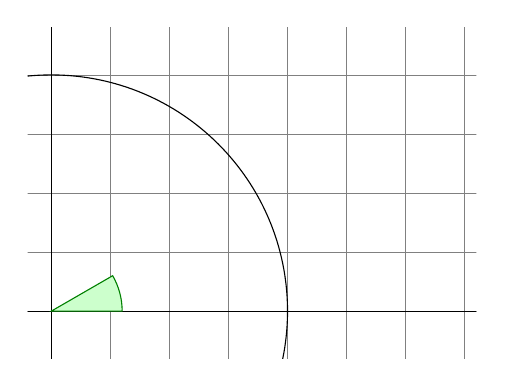
\begin{tikzpicture}[scale=3]
  \clip (-0.1,-0.2)
     rectangle (1.8,1.2);
  \draw[step=.25cm,gray,very thin]
       (-1.4,-1.4) grid (3.4,3.4);
  \draw (-1.5,0) -- (2.5,0);
  \draw (0,-1.5) -- (0,1.5);
  \draw (0,0) circle (1cm);
  \filldraw[fill=green!20!white,
            draw=green!50!black]
    (0,0) -- (3mm,0mm) 
         arc (0:30:3mm) -- cycle;
\end{tikzpicture}
\end{example}
Remarquez l'usage du point-virgule \og \texttt{;} \fg. Il s�pare les
commandes individuelles.

Un simple diagramme de Venn.
\begin{example}
\shorthandoff{:}
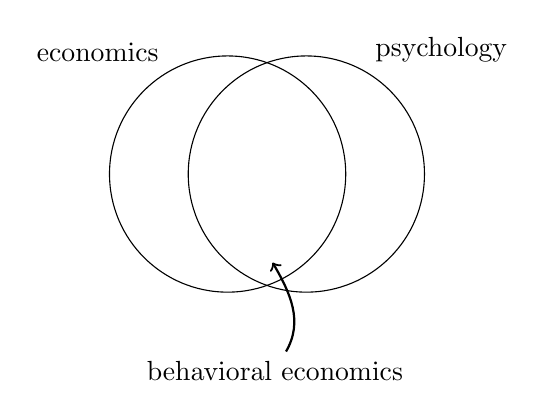
\begin{tikzpicture}
  \node[circle,draw,
        minimum size=3cm,
        label=120:{economics}]
         at (0,0) {};
  \node[circle,draw,
        minimum size=3cm,
        label=60:{psychology}]
         at (1,0) {};
  \node (i) at (0.5,-1) {};
  \node at (0.6,-2.5) 
    {behavioral economics}
    edge[->,thick,
         out=60,in=-60] (i);
\end{tikzpicture}
\end{example}
Si vous utilisez \pai{tikz} avec \pai{babel}, il se peut que certains
caract�res utilis�s par le langage TikZ soient modifi�s par \pai{babel}, ce
qui conduit � des erreurs �tranges. Pour �viter ce probl�me, ajoutez
la commande \ci{shorthandoff} � votre code.

Remarquez les boucles \og pour \fg (\texttt{foreach}) dans l'example suivant :
\begin{example}
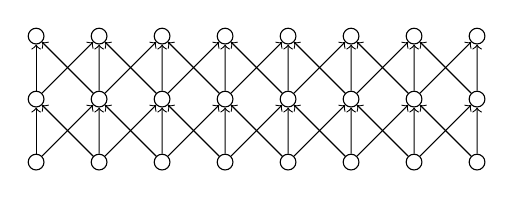
\begin{tikzpicture}[scale=0.8]
  \tikzstyle{v}=[circle, minimum size=2mm,inner sep=0pt,draw]
  \foreach \i in {1,...,8}
    \foreach \j in {1,...,3}
      \node[v] 
        (G-\i-\j) at (\i,\j) {};
  \foreach \i in {1,...,8}
    \foreach \j/\o in {1/2,2/3}
      \draw[->] 
        (G-\i-\j) -- (G-\i-\o);
  \foreach \i/\n in 
    {1/2,2/3,3/4,4/5,5/6,6/7,7/8}
    \foreach \j/\o in {1/2,2/3} {
       \draw[->] (G-\i-\j) -- (G-\n-\o);
       \draw[->] (G-\n-\j) -- (G-\i-\o);
    }
\end{tikzpicture}
\end{example}

Avec \ci{usetikzlibrary} dans le pr�ambule, vous pouvez activer de nombreuses
fonctionnalit�s pour le dessin de formes sp�ciales. Par exemple, la
biblioth�que \texttt{decorations.pathmorphing} permet d'obtenir des
bo�tes l�g�rement tordues.

\begin{example}
\usetikzlibrary{%
  decorations.pathmorphing}
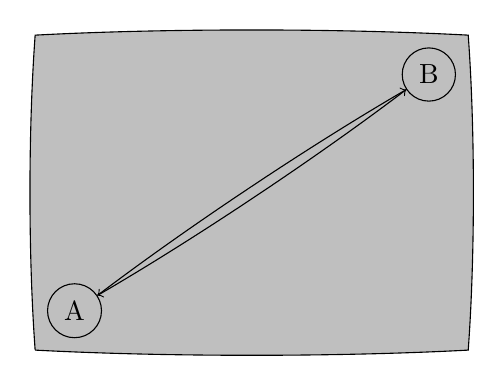
\begin{tikzpicture}[
     decoration={bent,aspect=.3}]
 \draw [decorate,fill=lightgray]
        (0,0) rectangle (5.5,4);
 \node[circle,draw] 
        (A) at (.5,.5) {A};
 \node[circle,draw] 
        (B) at (5,3.5) {B};
 \draw[->,decorate] (A) -- (B);
 \draw[->,decorate] (B) -- (A);
\end{tikzpicture}
\end{example}

\begin{example}
\usetikzlibrary{positioning}
\begin{tikzpicture}[xscale=6,
     yscale=8,>=stealth]
  \tikzstyle{v}=[circle,
     minimum size=1mm,draw,thick]
  \node[v] (a) {$1$};
  \node[v] (b) [right=of a] {$2$};
  \node[v] (c) [below=of a] {$2$};
  \node[v] (d) [below=of b] {$1$};
  \draw[thick,->] 
        (a) to node {} (c);
  \draw[thick,->] 
        (a) to node {} (d);
  \draw[thick,->] 
        (b) to node {} (d);
\end{tikzpicture}
\end{example}

Vous pouvez m�me dessiner des diagrammes syntaxiques comme s'ils provenaient
directement d'un livre sur la programmation Pascal. Le code est plus
complexe que l'exemple du dessus, aussi me contenterai-je de ne vous
montrer que son r�sultat. Si vous lisez la documentation de \pai{pgf}, vous
y trouverez un tutoriel pour dessiner ces m�mes diagrammes.

\begin{center}
\begin{tikzpicture}[point/.style={coordinate},thick,draw=black!50,>=stealth',
                    tip/.style={->,shorten >=1pt},every join/.style={rounded corners},
                    skip loop/.style={to path={-- ++(0,#1) -| (\tikztotarget)}},
                    hv path/.style={to path={-| (\tikztotarget)}},
                    vh path/.style={to path={|- (\tikztotarget)}},
                 terminal/.style={
            rounded rectangle,
            minimum size=6mm,
            thick,draw=black!50,
            top color=white,bottom color=black!20,
            font=\ttfamily\tiny},
                nonterminal/.style={
                       rectangle,
                       minimum size=6mm,
                       thick,
                       draw=red!50!black!50,         % 50% red and 50% black,
                       top color=white,              % a shading that is white at the top...
                       bottom color=red!50!black!20, % and something else at the bottom
                       font=\itshape\tiny}]
\matrix[column sep=3.5mm] {
  %MPG: pass� de 4 � 3.5mm, �a fait rentrer le truc dans la page...
  % First row:
  & & & & & & & & & & & \node (plus) [terminal] {+};\\
  % Second row:
  \node (p1) [point] {}; &     \node (ui1)    [nonterminal] {unsigned integer}; &
  \node (p2) [point] {}; &     \node (dot)    [terminal]    {.};                &
  \node (p3) [point] {}; &     \node (digit) [terminal]     {digit};            &
  \node (p4) [point] {}; &     \node (p5)     [point] {};                       &
  \node (p6) [point] {}; &     \node (e)      [terminal]    {E};                &
  \node (p7) [point] {}; &                                                      &
  \node (p8) [point] {}; &     \node (ui2)    [nonterminal] {unsigned integer}; &
  \node (p9) [point] {}; &     \node (p10)    [point]       {};\\
  % Third row:
  & & & & & & & & & & & \node (minus)[terminal] {-};\\
};
{ [start chain]
  \chainin (p1);
  \chainin (ui1)   [join=by tip];
  \chainin (p2)    [join];
  \chainin (dot)   [join=by tip];
  \chainin (p3)    [join];
  \chainin (digit) [join=by tip];
  \chainin (p4)    [join];
  { [start branch=digit loop]
    \chainin (p3) [join=by {skip loop=-6mm,tip}];
  }
  \chainin (p5)    [join,join=with p2 by {skip loop=6mm,tip}];
  \chainin (p6)    [join];
  \chainin (e)     [join=by tip];
  \chainin (p7)    [join];
  { [start branch=plus]
    \chainin (plus) [join=by {vh path,tip}];
    \chainin (p8)    [join=by {hv path,tip}];
  }
  { [start branch=minus]
    \chainin (minus) [join=by {vh path,tip}];
    \chainin (p8)    [join=by {hv path,tip}];
  }
  \chainin (p8)    [join];
  \chainin (ui2)   [join=by tip];
  \chainin (p9)    [join,join=with p6 by {skip loop=-11mm,tip}];
  \chainin (p10)   [join=by tip];
}
\end{tikzpicture}
\end{center}

Il y a bien plus : vous pouvez dessiner des graphes de donn�es
num�riques, de fonctions, etc � l'aide de l'extension
\pai{pgfplot}. Elle fournit tout ce dont vous avez besoin pour
dessiner des graphes. Elle peut m�me appeler la commande externe
\texttt{gnuplot} pour �valuer les fonctions faisant partie du graphe.

Pour encore plus d'inspiration, visitez l'�bahissant site de Kjell
Magne Fauske \url{http://www.texample.net/tikz/}. Il contient un
corpus toujours grandissant de beaux graphiques et de code \LaTeX{}.


%%% Local Variables:
%%% TeX-master: "lshort.tex"
%%% mode: flyspell
%%% TeX-PDF-mode: t
%%% End:

%%%%%%%%%%%%%%%%%%%%%%%%%%%%%%%%%%%%%%%%%%%%%%%%%%%%%%%%%%%%%%%%%
% Contents: Customising LaTeX output
% $Id$
%%%%%%%%%%%%%%%%%%%%%%%%%%%%%%%%%%%%%%%%%%%%%%%%%%%%%%%%%%%%%%%%%
\chapter{Customising \LaTeX}

\begin{intro}
Documents produced with the commands you have learned up to this
point will look acceptable to a large audience. While they are not
fancy-looking, they obey all the established rules of good
typesetting, which will make them easy to read and pleasant to look at.

However, there are situations where \LaTeX{} does not provide a
command or environment that matches your needs, or the output
produced by some existing command may not meet your requirements.

In this chapter, I will try to give some hints on
how to teach \LaTeX{} new tricks and how to make it produce output
that looks different from what is provided by default.
\end{intro}


\section{New Commands, Environments and Packages}

You may have noticed that all the commands I introduce in this
book are typeset in a box, and that they show up in the index at the end
of the book. Instead of directly using the necessary \LaTeX{} commands
to achieve this, I have created a \wi{package} in which I defined new
commands and environments for this purpose. Now I can simply write:

\begin{example}
\begin{lscommand}
\ci{dum}
\end{lscommand}
\end{example}

In this example, I am using both a new environment called\\
\ei{lscommand}, which is responsible for drawing the box around the
command, and a new command named \ci{ci}, which typesets the command
name and makes a corresponding entry in the index. Check
this out by looking up the \ci{dum} command in the index at the back
of this book, where you'll find an entry for \ci{dum}, pointing to
every page where I mentioned the \ci{dum} command.

If I ever decide that I do not like having the commands typeset in
a box any more, I can simply change the definition of the
\texttt{lscommand} environment to create a new look. This is much
easier than going through the whole document to hunt down all the
places where I have used some generic \LaTeX{} commands to draw a
box around some word. 


\subsection{New Commands}

To add your own commands, use the
\begin{lscommand}
\ci{newcommand}\verb|{|%
       \emph{name}\verb|}[|\emph{num}\verb|]{|\emph{definition}\verb|}|
\end{lscommand}
\noindent command. 
Basically, the command requires two arguments: the \emph{name} of the
command you want to create, and the \emph{definition} of the command.
The \emph{num} argument in square brackets is optional and specifies the number
of arguments the new command takes (up to 9 are possible).
If missing it defaults to 0, i.e. no argument allowed.

The following two examples should help you to get the idea.
The first example defines a new command called \ci{tnss}. This is
short for ``The Not So Short Introduction to \LaTeXe.'' Such a command
could come in handy if you had to write the title of this book over 
and over again. 

\begin{example}
\newcommand{\tnss}{The not
    so Short Introduction to
    \LaTeXe}
This is ``\tnss'' \ldots{} 
``\tnss''
\end{example}

The next example illustrates how to define a new
command that takes one argument.
The \verb|#1| tag gets replaced by the argument you specify.
If you wanted to use more than one argument, use \verb|#2| and
so on.

\begin{example}
\newcommand{\txsit}[2]
 {This is the \emph{#1} 
  #2 Introduction to \LaTeXe}
% in the document body: 
\begin{itemize}
\item \txsit{not so}{short}
\item \txsit{very}{long}
\end{itemize}
\end{example}

\LaTeX{} will not allow you to create a new command that would
overwrite an existing one. But there is a special command in case you
explicitly want this: \ci{renewcommand}.
It uses the same syntax as the \verb|\newcommand|
command.

In certain cases you might also want to use the \ci{providecommand}
command. It works like \ci{newcommand}, but if the command is
already defined, \LaTeXe{} will silently ignore it.

There are some points to note about whitespace following \LaTeX{} commands. See
page \pageref{whitespace} for more information.

\subsection{New Environments}
Just as with the \verb|\newcommand| command, there is a command
to create your own environments. The \ci{newenvironment} command uses the
following syntax:

\begin{lscommand}
\ci{newenvironment}\verb|{|%
       \emph{name}\verb|}[|\emph{num}\verb|]{|%
       \emph{before}\verb|}{|\emph{after}\verb|}|
\end{lscommand}

Again \ci{newenvironment} can have
an optional argument. The material specified
in the \emph{before} argument is processed before the text in the 
environment gets processed. The material in the \emph{after} argument gets
processed when the \verb|\end{|\emph{name}\verb|}| command is encountered.

The example below illustrates the usage of the \ci{newenvironment}
command. 
\begin{example}
\newenvironment{king}
 {\rule{1ex}{1ex}%
      \hspace{\stretch{1}}}
 {\hspace{\stretch{1}}%
      \rule{1ex}{1ex}}

\begin{king} 
My humble subjects \ldots
\end{king}
\end{example}

The \emph{num} argument is used the same way as in the
\verb|\newcommand| command. \LaTeX{} makes sure that you do not define
an environment that already exists. If you ever want to change an
existing command, use the \ci{renewenvironment} command. It
uses the same syntax as the \ci{newenvironment} command.

The commands used in this example will be explained later. For the
\ci{rule} command see page \pageref{sec:rule}, for \ci{stretch} go to
page \pageref{cmd:stretch}, and more information on \ci{hspace} can be
found on page \pageref{sec:hspace}.

\subsection{Extra Space}

When creating a new environment you may easily get bitten by extra spaces
creeping in, which can potentially have fatal effects, for example when you
want to create a title environment which supresses its own indentation as
well as the one on the following paragraph. The \ci{ignorespaces} command in
the begin block of the environment will make it ignore any space after
executing the begin block. The end block is a bit more tricky as special
processing occurs at the end of an environment. With the
\ci{ignorespacesafterend} \LaTeX{} will issue an \ci{ignorespaces} after the
special `end' processing has occurred.

\begin{example}
\newenvironment{simple}%
 {\noindent}%
 {\par\noindent}

\begin{simple}
See the space\\to the left.
\end{simple}
Same\\here.
\end{example}

\begin{example}
\newenvironment{correct}%
 {\noindent\ignorespaces}%
 {\par\noindent%
   \ignorespacesafterend}

\begin{correct}
No space\\to the left.
\end{correct}
Same\\here.
\end{example}

\subsection{Commandline \LaTeX}

If you work on a Unix-like OS, you might be using Makefiles to build your
\LaTeX{} projects. In that connection it might be interesting to produce
different versions of the same document by calling \LaTeX{} with commandline
parameters. If you add the following structure to your document:

\begin{verbatim}
\usepackage{ifthen}
\ifthenelse{\equal{\blackandwhite}{true}}{
  % "black and white" mode; do something..
}{
  % "color" mode; do something different..
}
\end{verbatim}

Now call \LaTeX{} like this:
\begin{verbatim}
latex '\newcommand{\blackandwhite}{true}\input{test.tex}'
\end{verbatim}

First the command \verb|\blackandwhite| gets defined and then the actual file is read with input.
By setting \verb|\blackandwhite| to false the color version of the document would be produced.

\subsection{Your Own Package}

If you define a lot of new environments and commands, the preamble of
your document will get quite long. In this situation, it is a good
idea to create a \LaTeX{} package containing all your command and
environment definitions. Use the \ci{usepackage}
command to make the package available in your document.

\begin{figure}[!htbp]
\begin{lined}{\textwidth}
\begin{verbatim}
% Demo Package by Tobias Oetiker
\ProvidesPackage{demopack}
\newcommand{\tnss}{The not so Short Introduction 
                   to \LaTeXe}
\newcommand{\txsit}[1]{The \emph{#1} Short 
                       Introduction to \LaTeXe}
\newenvironment{king}{\begin{quote}}{\end{quote}}
\end{verbatim}
\end{lined}
\caption{Example Package.} \label{package}
\end{figure}

Writing a package basically consists of copying the contents of
your document preamble into a separate file with a name ending in
\texttt{.sty}. There is one special command,
\begin{lscommand}
\ci{ProvidesPackage}\verb|{|\emph{package name}\verb|}|
\end{lscommand}
\noindent for use at the very beginning of your package
file. \verb|\ProvidesPackage| tells \LaTeX{} the name of the package
and will allow it to issue a sensible error message when you try to
include a package twice. Figure~\ref{package} shows a small example
package that contains the commands defined in the examples above.

\section{Fonts and Sizes}
\label{sec:fontsize}

\subsection{Font Changing Commands}
\index{font}\index{font size} \LaTeX{} chooses the appropriate font
and font size based on the logical structure of the document
(sections, footnotes, \ldots).  In some cases, one might like to change
fonts and sizes by hand. To do this, use the commands listed in
Tables~\ref{fonts} and~\ref{sizes}. The actual size of each font
is a design issue and depends on the document class and its options. 
Table~\ref{tab:pointsizes} shows the absolute point size for these
commands as implemented in the standard document classes.

\begin{example}
{\small The small and 
\textbf{bold} Romans ruled}
{\Large all of great big 
\textit{Italy}.}
\end{example}

One important feature of \LaTeXe{} is that the font attributes are
independent. This means that issuing size or even font
changing commands, and still keep bold or slant attributes set
earlier.

In \emph{math mode} use the font changing \emph{commands} to
temporarily exit \emph{math mode} and enter some normal text. If you want to
switch to another font for math typesetting you need another
special set of commands; refer to Table~\ref{mathfonts}.

\begin{table}[!bp]
\caption{Fonts.} \label{fonts}
\begin{lined}{12cm}
%
% Alan suggested not to tell about the other form of the command
% eg \verb|\sffamily| or \verb|\bfseries|. This seems a good thing to me.
%
\begin{tabular}{@{}rl@{\qquad}rl@{}}
\fni{textrm}\verb|{...}|        &      \textrm{\wi{roman}}&
\fni{textsf}\verb|{...}|        &      \textsf{\wi{sans serif}}\\
\fni{texttt}\verb|{...}|        &      \texttt{typewriter}\\[6pt]
\fni{textmd}\verb|{...}|        &      \textmd{medium}&
\fni{textbf}\verb|{...}|        &      \textbf{\wi{bold face}}\\[6pt]
\fni{textup}\verb|{...}|        &       \textup{\wi{upright}}&
\fni{textit}\verb|{...}|        &       \textit{\wi{italic}}\\
\fni{textsl}\verb|{...}|        &       \textsl{\wi{slanted}}&
\fni{textsc}\verb|{...}|        &       \textsc{\wi{Small Caps}}\\[6pt]
\ci{emph}\verb|{...}|          &            \emph{emphasized} &
\fni{textnormal}\verb|{...}|    &    \textnormal{document} font
\end{tabular}

\bigskip
\end{lined}
\end{table}


\begin{table}[!bp]
\index{font size}
\caption{Font Sizes.} \label{sizes}
\begin{lined}{12cm}
\begin{tabular}{@{}ll}
\fni{tiny}      & \tiny        tiny font \\
\fni{scriptsize}   & \scriptsize  very small font\\
\fni{footnotesize} & \footnotesize  quite small font \\
\fni{small}        &  \small            small font \\
\fni{normalsize}   &  \normalsize  normal font \\
\fni{large}        &  \large       large font
\end{tabular}%
\qquad\begin{tabular}{ll@{}}
\fni{Large}        &  \Large       larger font \\[5pt]
\fni{LARGE}        &  \LARGE       very large font \\[5pt]
\fni{huge}         &  \huge        huge \\[5pt]
\fni{Huge}         &  \Huge        largest
\end{tabular}

\bigskip
\end{lined}
\end{table}

\begin{table}[!tbp]
\caption{Absolute Point Sizes in Standard Classes.}\label{tab:pointsizes}
\label{tab:sizes}
\begin{lined}{12cm}
\begin{tabular}{lrrr}
\multicolumn{1}{c}{size} &
\multicolumn{1}{c}{10pt (default) } &
           \multicolumn{1}{c}{11pt option}  &
           \multicolumn{1}{c}{12pt option}\\
\verb|\tiny|       & 5pt  & 6pt & 6pt\\
\verb|\scriptsize| & 7pt  & 8pt & 8pt\\
\verb|\footnotesize| & 8pt & 9pt & 10pt \\
\verb|\small|        & 9pt & 10pt & 11pt \\
\verb|\normalsize| & 10pt & 11pt & 12pt \\
\verb|\large|      & 12pt & 12pt & 14pt \\
\verb|\Large|      & 14pt & 14pt & 17pt \\
\verb|\LARGE|      & 17pt & 17pt & 20pt\\
\verb|\huge|       & 20pt & 20pt & 25pt\\
\verb|\Huge|       & 25pt & 25pt & 25pt\\
\end{tabular}

\bigskip
\end{lined}
\end{table}


\begin{table}[!bp]
\caption{Math Fonts.} \label{mathfonts}
\begin{lined}{0.7\textwidth}
\begin{tabular}{@{}ll@{}}
\fni{mathrm}\verb|{...}|&     $\mathrm{Roman\ Font}$\\
\fni{mathbf}\verb|{...}|&     $\mathbf{Boldface\ Font}$\\
\fni{mathsf}\verb|{...}|&     $\mathsf{Sans\ Serif\ Font}$\\
\fni{mathtt}\verb|{...}|&     $\mathtt{Typewriter\ Font}$\\
\fni{mathit}\verb|{...}|&     $\mathit{Italic\ Font}$\\
\fni{mathcal}\verb|{...}|&    $\mathcal{CALLIGRAPHIC\ FONT}$\\
\fni{mathnormal}\verb|{...}|& $\mathnormal{Normal\ Font}$\\
\end{tabular}

%\begin{tabular}{@{}lll@{}}
%\textit{Command}&\textit{Example}&    \textit{Output}\\[6pt]
%\fni{mathcal}\verb|{...}|&    \verb|$\mathcal{B}=c$|&     $\mathcal{B}=c$\\
%\fni{mathscr}\verb|{...}|&    \verb|$\mathscr{B}=c$|&     $\mathscr{B}=c$\\
%\fni{mathrm}\verb|{...}|&     \verb|$\mathrm{K}_2$|&      $\mathrm{K}_2$\\
%\fni{mathbf}\verb|{...}|&     \verb|$\sum x=\mathbf{v}$|& $\sum x=\mathbf{v}$\\
%\fni{mathsf}\verb|{...}|&     \verb|$\mathsf{G\times R}$|&        $\mathsf{G\times R}$\\
%\fni{mathtt}\verb|{...}|&     \verb|$\mathtt{L}(b,c)$|&   $\mathtt{L}(b,c)$\\
%\fni{mathnormal}\verb|{...}|& \verb|$\mathnormal{R_{19}}\neq R_{19}$|&
%$\mathnormal{R_{19}}\neq R_{19}$\\
%\fni{mathit}\verb|{...}|&     \verb|$\mathit{ffi}\neq ffi$|& $\mathit{ffi}\neq ffi$
%\end{tabular}

\bigskip
\end{lined}
\end{table}

In connection with the font size commands, \wi{curly braces} play a
significant role. They are used to build \emph{groups}.  Groups
limit the scope of most \LaTeX{} commands.\index{grouping}

\begin{example}
He likes {\LARGE large and 
{\small small} letters}. 
\end{example}
 
The font size commands also change the line spacing, but only if the
paragraph ends within the scope of the font size command. The closing curly
brace \verb|}| should therefore not come too early.  Note the position of
the \ci{par} command in the next two examples. \footnote{\texttt{\bs{}par}
is equivalent to a blank line}


\begin{example}
{\Large Don't read this! 
 It is not true.
 You can believe me!\par}
\end{example}

\begin{example}
{\Large This is not true either.
But remember I am a liar.}\par
\end{example}

If you want to activate a size changing command for a whole paragraph
of text or even more, you might want to use the environment syntax for
font changing commands.

\begin{example}
\begin{Large} 
This is not true.
But then again, what is these
days \ldots
\end{Large}
\end{example}

\noindent This will save you from counting lots of curly braces.

\subsection{Danger, Will Robinson, Danger}

As noted at the beginning of this chapter, it is dangerous to clutter
your document with explicit commands like this, because they work in
opposition to the basic idea of \LaTeX{}, which is to separate the
logical and visual markup of your document.  This means that if you
use the same font changing command in several places in order to
typeset a special kind of information, you should use
\verb|\newcommand| to define a ``logical wrapper command'' for the font
changing command.

\begin{example}
\newcommand{\oops}[1]{%
 \textbf{#1}}
Do not \oops{enter} this room,
it's occupied by \oops{machines}
of unknown origin and purpose.
\end{example}

This approach has the advantage that you can decide at some later
stage that you want to use a visual representation of danger other
than \verb|\textbf|, without having to wade through your document,
identifying all the occurrences of \verb|\textbf| and then figuring out
for each one whether it was used for pointing out danger or for some other
reason.

Please note the difference between telling \LaTeX{} to
\emph{emphasize} something and telling it to use a different
\emph{font}. The \ci{emph} command is context aware, while the font commands are absolute.

\begin{example}
\textit{You can also
  \emph{emphasize} text if 
  it is set in italics,}
\textsf{in a 
  \emph{sans-serif} font,}
\texttt{or in 
  \emph{typewriter} style.}
\end{example}

\subsection{Advice}

To conclude this journey into the land of fonts and font sizes,
here is a little word of advice:\nopagebreak

\begin{quote}
  \underline{\textbf{Remember\Huge!}} \textit{The}
  \textsf{M\textbf{\LARGE O} \texttt{R}\textsl{E}} fonts \Huge you
  \tiny use \footnotesize \textbf{in} a \small \texttt{document},
  \large \textit{the} \normalsize more \textsc{readable} and
  \textsl{\textsf{beautiful} it bec\large o\Large m\LARGE e\huge s}.
\end{quote}

\section{Spacing}
 
\subsection{Line Spacing}

\index{line spacing} If you want to use larger inter-line spacing in a
document, change its value by putting the
\begin{lscommand}
\ci{linespread}\verb|{|\emph{factor}\verb|}|
\end{lscommand}
\noindent command into the preamble of your document.
Use \verb|\linespread{1.3}| for ``one and a half'' line
spacing, and \verb|\linespread{1.6}| for ``double'' line spacing.  Normally
the lines are not spread, so the default line spread factor
is~1.\index{double line spacing}

Note that the effect of the \ci{linespread} command is rather drastic and     
not appropriate for published work. So if you have a good reason for
changing the line spacing you might want to use the command:
\begin{lscommand}
\verb|\setlength{\baselineskip}{1.5\baselineskip}|
\end{lscommand}

\begin{example}
{\setlength{\baselineskip}%
           {1.5\baselineskip}
This paragraph is typeset with
the baseline skip set to 1.5 of
what it was before. Note the par
command at the end of the
paragraph.\par}

This paragraph has a clear
purpose, it shows that after the
curly brace has been closed,
everything is back to normal.
\end{example}

\subsection{Paragraph Formatting}\label{parsp}

In \LaTeX{}, there are two parameters influencing paragraph layout.
By placing a definition like
\begin{code}
\ci{setlength}\verb|{|\ci{parindent}\verb|}{0pt}| \\
\verb|\setlength{|\ci{parskip}\verb|}{1ex plus 0.5ex minus 0.2ex}|
\end{code}
in the preamble of the input file, you can change the layout of
paragraphs. These two commands increase the space between two paragraphs
while setting the paragraph indent to zero.  

The \texttt{plus} and \texttt{minus} parts of the length above tell
\TeX{} that it can compress and expand the inter-paragraph skip by the
amount specified, if this is necessary to properly fit the paragraphs
onto the page.

In continental Europe,
paragraphs are often separated by some space and not indented. But
beware, this also has its effect on the table of contents. Its lines
get spaced more loosely now as well. To avoid this, you might want to
move the two commands from the preamble into your document to some
place below the command \verb|\tableofcontents| or to not use them at all,
because you'll find that most professional books use indenting and not
spacing to separate paragraphs.


If you want to indent a paragraph that is not indented, use 
\begin{lscommand}
\ci{indent}
\end{lscommand}
\noindent at the beginning of the paragraph.\footnote{To indent the first paragraph after each section head, use
  the \pai{indentfirst} package in the `tools' bundle.} Obviously,
this will only have an effect when \verb|\parindent| is not set to
zero.

To create a non-indented paragraph, use 
\begin{lscommand}
\ci{noindent}
\end{lscommand}
\noindent as the first command of the paragraph. This might come in handy when
you start a document with body text and not with a sectioning command.

\subsection{Horizontal Space}

\label{sec:hspace}
\LaTeX{} determines the spaces between words and sentences
automatically. To add horizontal space, use: \index{horizontal!space}
\begin{lscommand}
\ci{hspace}\verb|{|\emph{length}\verb|}|
\end{lscommand}
If such a space should be kept even if it falls at the end or the
start of a line, use \verb|\hspace*| instead of \verb|\hspace|.  The
\emph{length} in the simplest case is just a number plus a unit.  The
most important units are listed in Table~\ref{units}. 
\index{units}\index{dimensions}

\begin{example}
This\hspace{1.5cm}is a space 
of 1.5 cm. 
\end{example}
\suppressfloats
\begin{table}[tbp]
\caption{\TeX{} Units.} \label{units}\index{units}
\begin{lined}{9.5cm} 
\begin{tabular}{@{}ll@{}}
\texttt{mm} & millimetre $\approx 1/25$~inch \quad \demowidth{1mm} \\
\texttt{cm} & centimetre = 10~mm  \quad \demowidth{1cm}                     \\
\texttt{in} & inch $=$ 25.4~mm \quad \demowidth{1in}                    \\
\texttt{pt} & point $\approx 1/72$~inch $\approx \frac{1}{3}$~mm  \quad\demowidth{1pt}\\
\texttt{em} & approx width of an `M' in the current font \quad \demowidth{1em}\\
\texttt{ex} & approx height of an `x' in the current font \quad \demowidth{1ex}
\end{tabular}

\bigskip
\end{lined}
\end{table}

\label{cmd:stretch} 
The command
\begin{lscommand}
\ci{stretch}\verb|{|\emph{n}\verb|}|
\end{lscommand} 
\noindent generates a special rubber space. It stretches until all the
remaining space on a line is filled up. If multiple
\verb|\hspace{\stretch{|\emph{n}\verb|}}| commands are issued on the same
line, they occupy all available space in proportion of their respective
stretch factors.


\begin{example}
x\hspace{\stretch{1}}
x\hspace{\stretch{3}}x
\end{example}

When using horizontal space together with text, it may make sense to make
the space adjust its size relative to the size of the current font.
This can be done by using the text-relative units \texttt{em} and
\texttt{ex}:

\begin{example}
{\Large{}big\hspace{1em}y}\\
{\tiny{}tin\hspace{1em}y}
\end{example}
 
\subsection{Vertical Space}
The space between paragraphs, sections, subsections, \ldots\ is
determined automatically by \LaTeX. If necessary, additional vertical
space \emph{between two paragraphs} can be added with the command:
\begin{lscommand}
\ci{vspace}\verb|{|\emph{length}\verb|}|
\end{lscommand}

This command should normally be used between two empty lines.  If the
space should be preserved at the top or at the bottom of a page, use
the starred version of the command, \verb|\vspace*|, instead of \verb|\vspace|.
\index{vertical space}

The \verb|\stretch| command, in connection with \verb|\pagebreak|, can
be used to typeset text on the last line of a page, or to centre text
vertically on a page.
\begin{code}
\begin{verbatim}
Some text \ldots

\vspace{\stretch{1}}
This goes onto the last line of the page.\pagebreak
\end{verbatim}
\end{code}

Additional space between two lines of \emph{the same} paragraph or
within a table is specified with the
\begin{lscommand}
\ci{\bs}\verb|[|\emph{length}\verb|]|
\end{lscommand}
\noindent command. 

With \ci{bigskip} and \ci{smallskip} you can skip a predefined amount of
vertical space without having to worry about exact numbers.


\section{Page Layout}

\begin{figure}[!hp]
\begin{center}
\makeatletter\@mylayout\makeatother
\end{center}
\vspace*{1.8cm}
\caption[Layout parameters for this book.]{Layout parameters for this book. Try the \pai{layouts} package to print the layout of your own document.}
\label{fig:layout}
\cih{footskip}
\cih{headheight}
\cih{headsep}
\cih{marginparpush}
\cih{marginparsep}
\cih{marginparwidth}
\cih{oddsidemargin}
\cih{paperheight}
\cih{paperwidth}
\cih{textheight}
\cih{textwidth}
\cih{topmargin}
\end{figure}
\index{page layout}
\LaTeXe{} allows you to specify the \wi{paper size} in the
\verb|\documentclass| command. It then automatically picks the right 
text \wi{margins}, but sometimes you may not be happy with 
the predefined values. Naturally, you can change them. 
%no idea why this is needed here ...
\thispagestyle{fancyplain}
Figure~\ref{fig:layout} shows all the parameters that can be changed.
The figure was produced with the \pai{layout} package from the tools bundle.%
\footnote{\CTANref|pkg/tools|}

\textbf{WAIT!} \ldots before you launch into a ``Let's make that
narrow page a bit wider'' frenzy, take a few seconds to think. As with
most things in \LaTeX, there is a good reason for the page layout to
be as it is.

Sure, compared to your off-the-shelf MS Word page, it looks awfully
narrow. But take a look at your favourite book\footnote{I mean a real
  printed book produced by a reputable publisher.} and count the number
of characters on a standard text line. You will find that there are no
more than about 66 characters on each line. Now do the same on your
\LaTeX{} page. You will find that there are also about 66 characters
per line.  Experience shows that the reading gets difficult as soon as
there are more characters on a single line. This is because it is
difficult for the eyes to move from the end of one line to the start of the next one.
This is also why newspapers are typeset in multiple columns.

So if you increase the width of your body text, keep in mind that you
are making life difficult for the readers of your paper. But enough
of the cautioning, I promised to tell you how you do it \ldots
 
\LaTeX{} provides two commands to change these parameters. They are
usually used in the document preamble.

The first command assigns a fixed value to any of the parameters:
\begin{lscommand}
\ci{setlength}\verb|{|\emph{parameter}\verb|}{|\emph{length}\verb|}|
\end{lscommand}

The second command adds a length to any of the parameters:
\begin{lscommand}
\ci{addtolength}\verb|{|\emph{parameter}\verb|}{|\emph{length}\verb|}|
\end{lscommand} 

This second command is actually more useful than the \ci{setlength}
command, because it works relative to the existing settings.
To add one centimetre to the overall text width, I put the
following commands into the document preamble:
\begin{code}
\verb|\addtolength{\hoffset}{-0.5cm}|\\
\verb|\addtolength{\textwidth}{1cm}|
\end{code}

In this context, you might want to look at the \pai{calc} package.
It allows you to use arithmetic operations in the argument of \ci{setlength}
and other places where numeric values are entered into function
arguments.

\section{More Fun With Lengths}

Whenever possible, I avoid using absolute lengths in
\LaTeX{} documents. I rather try to base things on the width or height
of other page elements. For the width of a figure this could
be \verb|\textwidth| in order to make it fill the page.

The following 3 commands allow you to determine the width, height and
depth of a text string.

\begin{lscommand}
\ci{settoheight}\verb|{|\emph{variable}\verb|}{|\emph{text}\verb|}|\\
\ci{settodepth}\verb|{|\emph{variable}\verb|}{|\emph{text}\verb|}|\\
\ci{settowidth}\verb|{|\emph{variable}\verb|}{|\emph{text}\verb|}|
\end{lscommand}

\noindent The example below shows a possible application of these commands.

\begin{example}
\flushleft
\newenvironment{vardesc}[1]{%
  \settowidth{\parindent}{#1:\ }
  \makebox[0pt][r]{#1:\ }}{}

\begin{displaymath}
a^2+b^2=c^2
\end{displaymath}

\begin{vardesc}{Where}$a$, 
$b$ -- are adjacent to the right 
angle of a right-angled triangle.  

$c$ -- is the hypotenuse of 
the triangle and feels lonely.

$d$ -- finally does not show up 
here at all. Isn't that puzzling?
\end{vardesc}
\end{example}

\section{Boxes}
\LaTeX{} builds up its pages by pushing around boxes. At first, each
letter is a little box, which is then glued to other letters to form
words. These are again glued to other words, but with special glue,
which is elastic so that a series of words can be squeezed or
stretched as to exactly fill a line on the page. 

I admit, this is a very simplistic version of what really happens, but the
point is that \TeX{} operates on glue and boxes. Letters are not the only
things that can be boxes. You can put virtually everything into a box,
including other boxes. Each box will then be handled by \LaTeX{} as if it
were a single letter.

In earlier chapters you encountered some boxes, although I did
not tell you. The \ei{tabular} environment and the \ci{includegraphics}, for
example, both produce a box. This means that you can easily arrange two
tables or images side by side. You just have to make sure that their
combined width is not larger than the textwidth.

You can also pack a paragraph of your choice into a box with either
the

\begin{lscommand}
\ci{parbox}\verb|[|\emph{pos}\verb|]{|\emph{width}\verb|}{|\emph{text}\verb|}|
\end{lscommand}

\noindent command or the

\begin{lscommand}
\verb|\begin{|\ei{minipage}\verb|}[|\emph{pos}\verb|]{|\emph{width}\verb|}| text
\verb|\end{|\ei{minipage}\verb|}|
\end{lscommand}

\noindent environment. The \texttt{pos} parameter can take one of the letters
\texttt{c, t} or \texttt{b} to control the vertical alignment of the box,
relative to the baseline of the surrounding text. \texttt{width} takes
a length argument specifying the width of the box. The main difference
between a \ei{minipage} and a \ci{parbox} is that you cannot use all commands
and environments inside a \ei{parbox}, while almost anything is possible in
a \ei{minipage}.

While \ci{parbox} packs up a whole paragraph doing line breaking and
everything, there is also a class of boxing commands that operates
only on horizontally aligned material. We already know one of them;
it's called \ci{mbox}. It simply packs up a series of boxes into
another one, and can be used to prevent \LaTeX{} from breaking two
words. As boxes can be put inside boxes, these horizontal box packers
give you ultimate flexibility.

\begin{lscommand}
\ci{makebox}\verb|[|\emph{width}\verb|][|\emph{pos}\verb|]{|\emph{text}\verb|}|
\end{lscommand}

\noindent \texttt{width} defines the width of the resulting box as
seen from the outside.\footnote{This means it can be smaller than the
material inside the box. You can even set the
width to 0pt so that the text inside the box will be typeset without
influencing the surrounding boxes.}  Besides the length
expressions, you can also use \ci{width}, \ci{height}, \ci{depth}, and
\ci{totalheight} in the width parameter. They are set from values
obtained by measuring the typeset \emph{text}. The \emph{pos} parameter takes
a one letter value: \textbf{c}enter, flush\textbf{l}eft,
flush\textbf{r}ight, or \textbf{s}pread the text to fill the box.

The command \ci{framebox} works exactly the same as \ci{makebox}, but
it draws a box around the text.

The following example shows you some things you could do with
the \ci{makebox} and \ci{framebox} commands.

\begin{example}
\makebox[\textwidth]{%
    c e n t r a l}\par
\makebox[\textwidth][s]{%
    s p r e a d}\par
\framebox[1.1\width]{Guess I'm 
    framed now!} \par
\framebox[0.8\width][r]{Bummer, 
    I am too wide} \par
\framebox[1cm][l]{never 
    mind, so am I} 
Can you read this?
\end{example}

Now that we control the horizontal, the obvious next step is to go for
  the vertical.\footnote{Total control is only to be obtained by
  controlling both the horizontal and the vertical \ldots}
 No problem for \LaTeX{}. The


\begin{lscommand}
\ci{raisebox}\verb|{|\emph{lift}\verb|}[|\emph{extend-above-baseline}\verb|][|\emph{extend-below-baseline}\verb|]{|\emph{text}\verb|}|
\end{lscommand}

\noindent command lets you define the vertical properties of a
box. You can use \ci{width}, \ci{height}, \ci{depth}, and
  \ci{totalheight} in the first three parameters, in order to act
  upon the size of the box inside the \emph{text} argument.


\begin{example}
\raisebox{0pt}[0pt][0pt]{\Large%
\textbf{Aaaa\raisebox{-0.3ex}{a}%
\raisebox{-0.7ex}{aa}%
\raisebox{-1.2ex}{r}%
\raisebox{-2.2ex}{g}%
\raisebox{-4.5ex}{h}}}
she shouted, but not even the next
one in line noticed that something
terrible had happened to her.
\end{example}

\section{Rules}
\label{sec:rule}

A few pages back you may have noticed the command

\begin{lscommand}
\ci{rule}\verb|[|\emph{lift}\verb|]{|\emph{width}\verb|}{|\emph{height}\verb|}|
\end{lscommand}

\noindent In normal use it produces a simple black box.

\begin{example}
\rule{3mm}{.1pt}%
\rule[-1mm]{5mm}{1cm}%
\rule{3mm}{.1pt}%
\rule[1mm]{1cm}{5mm}%
\rule{3mm}{.1pt}
\end{example}

\noindent This is useful for drawing vertical and horizontal
lines. The line on the title page, for example, has been created with a
\ci{rule} command.

\bigskip
{\flushright The End.\par}

%

% Local Variables:
% TeX-master: "lshort2e"
% mode: latex
% mode: flyspell
% End:

\appendix
\chapter{Installing \LaTeX}
\begin{intro}
Knuth published the source to \TeX{} back in a time when nobody knew
about OpenSource and/or Free Software. The License that comes with \TeX{}
lets you do whatever you want with the source, but you can only call the
result of your work \TeX{} if the program passes a set of tests Knuth has
also provided. This has lead to a situation where we have free \TeX{}
implementations for almost every Operating System under the sun. This chapter
will give some hints on what to install on Linux, Mac OS X and Windows, to
get a working \TeX{} setup.
\end{intro}

\section{What to Install}

For using \LaTeX{} on any computer system, you need several programs.

\begin{enumerate}

\item The \TeX{}/\LaTeX{} program for processing your \LaTeX{} source files
into typeset PDF or DVI documents.

\item A text editor for editing your \LaTeX{} source files. Some products even let
you start the \LaTeX{} program from within the editor.

\item A PDF/DVI viewer program for previewing and printing your
documents.

\item A program to handle \PSi{} files and images for inclusion into
your documents.

\end{enumerate}

For all platforms there are several programs that fit the requirements above.
Here we just tell about the ones we know, like and have some experience
with.

\section{Cross Platform Editor}

While \TeX{} is available on many different computing platforms, \LaTeX{}
editors have long been highly platform specific.

Over the past few years I have come to like Texmaker quite a lot.
Apart from being very a useful editor with integrated pdf-preview, syntax
high-lighting, it has the advantage of running on Windows, Mac and
Unix/Linux equally well.  See \url{http://www.xm1math.net/texmaker} for
further information.  Note there is also a forked version of Texmaker called
TeXstudio on \url{http://texstudio.sourceforge.net/}.  It also seems well
maintained and is also available for all three major platforms.

You will find some platform specific editor suggestions in the OS sectons below.

\section{\TeX{} on Mac OS X}

\subsection{\TeX{} Distribution}

Just download \wi{MacTeX}. It is a
pre-compiled \LaTeX{} distribution for OS X. \wi{MacTeX} provides a full \LaTeX{}
installation plus a number of additional tools. Get Mac\TeX{} from
\url{http://www.tug.org/mactex/}.

\subsection{OSX \TeX{} Editor}

If you are not happy with our crossplatform suggestion Texmaker (section \ref{sec:texmaker}).
 
The most popular open source editor for \LaTeX{} on the mac seems to be
\TeX{}shop.  Get a copy from \url{http://www.uoregon.edu/~koch/texshop}. It
is also contained in the \wi{MacTeX} distribution.

Recent \TeX Live distributions contain the \TeX{}works editor 
\url{http://texworks.org/} which is a multi-platform editor based on the \TeX{}Shop
design. Since \TeX{}works uses the Qt toolkit, it is available on any platform
supported by this toolkit (MacOS X, Windows, Linux.) 

\subsection{Treat yourself to \wi{PDFView}}

Use PDFView for viewing PDF files generated by \LaTeX{}, it integrates tightly
with your \LaTeX{} text editor. PDFView is an open-source application, available from the PDFView website on\\
\url{http://pdfview.sourceforge.net/}. After installing, open
PDFViews preferences dialog and make sure that the \emph{automatically reload
documents} option is enabled and that PDFSync support is set appropriately.

\section{\TeX{} on Windows}

\subsection{Getting \TeX{}}

First, get a copy of the excellent MiK\TeX\index{MiKTeX@MiK\TeX} distribution from\\
\url{http://www.miktex.org/}. It contains all the basic programs and files
required to compile \LaTeX{} documents.  The coolest feature in my eyes, is
that MiK\TeX{} will download missing \LaTeX{} packages on the fly and install them
magically while compiling a document. Alternatively you can also use
the TeXlive distribution which exists for Windows, Unix and Mac OS to
get your base setup going \url{http://www.tug.org/texlive/}.

\subsection{A \LaTeX{} editor}

If you are not happy with our crossplatform suggestion Texmaker (section \ref{sec:texmaker}).

\wi{TeXnicCenter} uses many concepts from the programming-world to provide a nice and
efficient \LaTeX{} writing environment in Windows. Get your copy from\\
\url{http://www.texniccenter.org/}. TeXnicCenter integrates nicely with
MiKTeX.

Recent \TeX Live distributions contain the \TeX{}works Editor
\url{http://texworks.org/}. It supports Unicode and requires at least Windows XP.

\subsection{Document Preview}

You will most likely be using Yap for DVI preview as it gets installed with
MikTeX. For PDF you may want to look at Sumatra
PDF \url{http://blog.kowalczyk.info/software/sumatrapdf/}. I mention Sumatra PDF
because it lets you jump from any position in the pdf document back into
corresponding position in your source document.

\subsection{Working with graphics}

Working with high quality graphics in \LaTeX{} means that you have to use
\EPSi{} (eps) or PDF as your picture format. The program that helps you
deal with this is called \wi{GhostScript}. You can get it, together with its
own front-end \wi{GhostView}, from \url{http://www.cs.wisc.edu/~ghost/}.

If you deal with bitmap graphics (photos and scanned material), you may want
to have a look at the open source Photoshop alternative \wi{Gimp}, available
from \url{http://gimp-win.sourceforge.net/}.

\section{\TeX{} on Linux}

If you work with Linux, chances are high that \LaTeX{} is already installed
on your system, or at least available on the installation source you used to
setup. Use your package manager to install the following packages:

\begin{itemize}
\item texlive -- the base \TeX{}/\LaTeX{} setup.
\item emacs (with AUCTeX) -- an editor that integrates tightly with \LaTeX{} through the add-on AUCTeX package.
\item ghostscript -- a \PSi{} preview program.
\item xpdf and acrobat -- a PDF preview program.
\item imagemagick -- a free program for converting bitmap images.
\item gimp -- a free Photoshop look-a-like.
\item inkscape -- a free illustrator/corel draw look-a-like.
\end{itemize}

If you are looking for a more windows like graphical editing environment,
check out Texmaker. See section \ref{sec:texmaker}.

Most Linux distros insist on splitting up their \TeX{} environments into a
large number of optional packages, so if something is missing after your
first install, go check again.

\backmatter
%%%%%%%%%%%%%%%%%%%%%%%%%%%%%%%%%%%%%%%%%%%%%%%%%%%%%%%%%%%%%%%%%
% Contents: The Bibliography
% File: biblio.tex (lshort2e.tex)
% $Id: biblio.tex 449 2010-12-14 16:53:51Z oetiker $
%%%%%%%%%%%%%%%%%%%%%%%%%%%%%%%%%%%%%%%%%%%%%%%%%%%%%%%%%%%%%%%%%

% Pour les informations de licence, voir title.tex.
% See title.tex for license information.

\begin{thebibliography}{99}
\addcontentsline{toc}{chapter}{\bibname} 
\thispagestyle{plain}

\bibitem{manual} \textsc{Lamport}, Leslie.  \newblock \emph{{\LaTeX:}
    A Document Preparation System}.  \newblock Addison-Wesley, 1994.
    2\ieme{} �dition.\\ ISBN~0-201-52983-1.

\bibitem{texbook} \textsc{Knuth}, Donald~E.  \newblock 
    \textit{The \TeX{}book,} Volume~A de \textit{Computers and
    Typesetting}. Addison-Wesley, 1984.
    2\ieme{} �dition.\\
    ISBN~0-201-13448-9.

\bibitem{companion} \textsc{Mittelbach}, Frank ; \textsc{Goossens},
  Michel. Trad. supervis�e par Jacques \textsc{Andr�}
  \newblock \emph{le {\LaTeX} Companion, 2\ieme �dition}.  \newblock
  Pearson Education France, 2005.\\ ISBN~2-7440-7133-1.

\bibitem{graphicscompanion} Michel Goossens, Sebastian Rahtz and Frank
  Mittelbach.  \newblock \emph{The {\LaTeX} Graphics Companion}.  \newblock
  Addison-Wesley, Reading, Massachusetts, 1997, ISBN~0-201-85469-4.

\bibitem{desgraupes} \textsc{Desgraupes}, Bernard.
  \newblock \emph{{\LaTeX} Apprentissage, guide et r�f�rence}. \newblock
  Vuibert, 2000.\\
  ISBN~2-7117-8658-7.

\bibitem{local} Chaque installation de \LaTeX{} devrait fournir un 
  document appel�
  \emph{\LaTeX{} Local Guide} qui explique les particularit�s de
  cette installation. Malheureusement certains administrateurs syst�me
  paresseux ne fournissent pas ce document. Dans ce cas, demandez de
  l'aide aux
  autres utilisateurs autour de vous ou au gourou local de \LaTeX{}.

\bibitem{usrguide} \LaTeX3 Project Team.  \newblock \emph{\LaTeXe~for
    authors}.  \newblock Distribu� avec \LaTeXe{} dans
  \texttt{usrguide.tex}.

\bibitem{clsguide} \LaTeX3 Project Team.  \newblock \emph{\LaTeXe~for
    Class and Package writers}.  \newblock Distribu� avec \LaTeXe{} dans
   \texttt{clsguide.tex}.

\bibitem{fntguide} \LaTeX3 Project Team.  \newblock \emph{\LaTeXe~Font
    selection}.  \newblock Distribu� avec \LaTeXe{} dans
  \texttt{fntguide.tex}.

\bibitem{graphics} \textsc{Carlisle}, David~P. \newblock \emph{Packages in the
    `graphics' bundle}.  \newblock Distribu� avec les extensions
    � graphics � dans \texttt{grfguide.tex}.

\bibitem{verbatim} \textsc{Sch�pf}, Rainer ; \textsc{Raichle}, Bernd
    et \textsc{Rowley} Chris.  
    \newblock \emph{A New Implementation of \LaTeX's verbatim
    Environments}.
    \newblock Distribu� avec l'ensemble � tools � dans
    \texttt{verbatim.dtx}.

\bibitem{amsguide} American Mathematical Society \newblock
    \emph{\AmS-\LaTeX{} Version 1.2 User's guide}. \newblock Distribu�
    avec les extensions \AmS-\LaTeX{} dans \texttt{amsldoc.tex}. 

\bibitem{french} \textsc{Gaulle}, Bernard. \newblock \emph{Notice 
  d'utilisation du style french multilingue}. \newblock Disponible
  avec l'extension \texttt{french} sur \texttt{http://frenchpro.free.fr/}.

\bibitem{ftypo} \textsc{Perrousseaux}, Yves. \newblock \emph{Manuel de
  typographie fran�aise �l�mentaire}. \newblock Ateliers Perrousseaux
  �diteur, 1995.\\
  ISBN~2-911220-00-5.

\bibitem{cyrguide} Vladimir Volovich, Werner Lemberg and \LaTeX3 Project Team.
    \newblock \emph{Cyrillic languages support in \LaTeX}.
    \newblock Fourni avec la distribution \LaTeXe{} sous la forme du
    fichier \texttt{cyrguide.tex}.

\bibitem{catalogue} Graham~Williams.  \newblock \emph{The TeX
    Catalogue} is a very complete listing of many \TeX{} and \LaTeX{}
    related packages.
  \newblock Available online from \CTAN|help/Catalogue/catalogue.html|

\bibitem{eps} \textsc{Reckdahl}, Keith.  \newblock \emph{Using EPS Graphics in
    \LaTeXe{} Documents} qui explique tout ce que vous avez toujours
    voulu savoir et m�me plus sur les fichiers PostScript et leur
    utilisation avec \LaTeX{}. \newblock Disponible en ligne sur
    \CTAN|info/epslatex.ps|

\bibitem{xy-pic} Kristoffer H. Rose.
  \newblock \emph{\Xy-pic User's Guide}.  \newblock
  T�l�chargeable depuis le CTAN avec la distribution \Xy-pic

\bibitem{metapost} John D. Hobby.
  \newblock \emph{A User's Manual for \MP}. \newblock
  T�l�chargeable depuis \url{http://cm.bell-labs.com/who/hobby/} 

\bibitem{unbound} Alan Hoenig.
  \newblock \emph{\TeX{} Unbound}. \newblock Oxford University Press, 1998,
    ISBN 0-19-509685-1; 0-19-509686-X (pbk.) 

\bibitem{ursoswald} Urs Oswald.  
    \newblock \emph{Graphics in \LaTeXe{}}, contient des fichiers
    source Java pour g�n�rer des cercles et des ellipses arbitraires
    dans l'environnement \texttt{picture}, et \emph{\MP{} - A
      Tutorial}.
  \newblock Les deux sont t�l�chargeables depuis \url{http://www.ursoswald.ch}

\bibitem{pgfplot} Till Tantau.
  \newblock \emph{TikZ\&PGF Manual}.\newblock
  Download from \CTAN|graphics/pgf/base/doc/generic/pgf/pgfmanual.pdf|

% new items for XeLaTeX
\bibitem{polyglossia} Fran\c{c}ois Charette.
    \newblock \emph{Polyglossia: A Babel Replacement for \hologo{XeLaTeX}}.
    \newblock Comes with the \TeX Live distribution as
  \texttt{polyglossia.pdf}. (Type \texttt{texdoc polyglossia} on the command line.)

\bibitem{arabxetex} Fran\c{c}ois Charette.
    \newblock \emph{An Arab\TeX-like interface for typesetting languages
     in Arabic script with \hologo{XeLaTeX}}.
    \newblock Comes with the \TeX Live distribution as
  \texttt{arabxetex.pdf}. (Type \texttt{texdoc arabxetex} on the command line.)

\bibitem{fontspec} Will Robertson and Khaled Hosny.
    \newblock \emph{The \texttt{fontspec} package}.
    \newblock Comes with the \TeX Live distribution as
  \texttt{fontspec.pdf}. (Type \texttt{texdoc fontspec} on the command line.)

\bibitem{xgreek} Apostolos Syropoulos.
    \newblock \emph{The \texttt{xgreek} package}.
    \newblock Comes with the \TeX Live distribution as
  \texttt{xgreek.pdf}. (Type \texttt{texdoc xgreek} on the command line.)

\bibitem{bidi} Vafa Khalighi.
    \newblock \emph{The \texttt{bidi} package}.
    \newblock Comes with the \TeX Live distribution as
  \texttt{bidi.pdf}. (Type \texttt{texdoc bidi} on the command line.

\bibitem{xepersian} Vafa Khalighi.
    \newblock \emph{The \texttt{XePersian} package}.
    \newblock Comes with the \TeX Live distribution as
  \texttt{xepersian-doc.pdf}. (Type \texttt{texdoc xepersian} on the command line.

\bibitem{xecjk} Wenchang Sun.
    \newblock \emph{The \texttt{xeCJK} package}.
    \newblock Comes with the \TeX Live distribution as
  \texttt{xeCJK.pdf}. (Type \texttt{texdoc xecjk} on the command line.

\end{thebibliography}


%

% Local Variables:
% TeX-master: "lshort2e"
% mode: latex
% mode: flyspell
% End:

\refstepcounter{chapter}
\addcontentsline{toc}{chapter}{Index} 
\printindex
\end{document}





%

% Local Variables:
% TeX-master: "lshort2e"
% mode: latex
% mode: flyspell
% End:
